% University of Michigan Dissertation LaTeX Template for 2023
% Created by John Meluso and Shreyas Kousik
% 9 Jul 2020

% Use the University of Michigan thesis class.
\documentclass[thesis]{thesis-umich}
\input{packages}

%--- Set the font styles -----
% As of this writing, Rackham does not have strict font requirements, but they
% suggest "standard fonts" such as Times, Arial, or Times New Roman.
% In practice, they allow the default LaTeX font (Computer Modern).
% The fonts available to you depend on the typesetting engine you use, e.g.
% pdflatex (the overleaf default), xelatex, or lualatex.
% Set the font to whatever you like, as long as it's compatible with the tex
% engine you're using.
% More information from Overleaf on font selection with:
%     - pdflatex: https://www.overleaf.com/learn/latex/Font_typefaces
%     - xelatex: https://www.overleaf.com/learn/latex/XeLaTeX
% See examples below depending on your engine and uncomment the usepackage
% commands and any subsequent commands as needed.
%-------------------------------------------------------------------------------
%--- pdflatex -----
%\usepackage{times}
%\usepackage{newtxtext}
%\usepackage{newtxmath}
%-------------------------------------------------------------------------------
%--- xelatex / lualatex -----
%\usepackage{fontspec}
%\setromanfont{Times New Roman}
%\setsansfont{Arial}
%\setmonofont{Courier New}
%-------------------------------------------------------------------------------

% If you are using the alpha bibliography style, keep these next three lines in your preamble, so that the references are left-aligned; or, you can comment it out and see what happens
\makeatletter
\renewcommand{\@biblabel}[1]{[#1]\hfill}
\makeatother

% Title of the thesis
\title{Methods development toward non-equilibrium studies
of transcription initiation by \textit{E. coli} RNA Polymerase}

% Author name
\author{Maya A. Segal}

% Department
%\department{Chemistry}

% Year of completion
\year=2023

% Author email
\email{mayasegala@gmail.com}

% Author ORCID iD
\orcid{0000-0002-1828-7682}

% Frontispiece
% if you want to add a frontispiece, add an image named `frontispiece.png1
%\frontispiece{\includegraphics[width=4in]{front_materials/frontispiece.png}}

% Default style for front pages
\frontpagestyle{7} % 7 is preferred by Rackham, but should be set individually for each front page

% Dedication (the input [7] determines the style -- 7 is Rackham's preferred style)
% \hidededication{%
\dedication[7]{\vspace*{\fill}

\begin{center}
    To my loving husband, daughter, and son on the way, \\
    for making my life fuller than I could ever have dreamed,\\
    and for supporting me on my academic journey.
\end{center}

\vspace*{\fill}
}

% Acknowledgments (the input [7] determines the style -- 7 is Rackham's preferred style)
\acknowledgments[7]{\vspace*{\fill}

I am sincerely grateful for the guidance, mentorship, and inspiration provided by my advisor, Dr. Shimon Weiss. 
You been extremely supportive of me, even when it was a challenge to do so. 
You accepted me into your group when I was struggling with my coursework and never once made me feel inferior for my learning disabilities. 
When I had a medical emergency and my daughter was born three months early, 
you allowed me to work from home for an entire year.
I was able to protect her from COVID-19 when she was most at risk, and the time I spent with her was precious beyond measure.
I am truly grateful for your patience and support during my trying entrance to motherhood.
Without it, I would not be so fortunate as to find myself in this position now.
Last, and certainly not least, you respectfully guided me through my academic journey, and for that I am eternally thankful. 

In addition, I would like to thank Dr. Xavier Michalet, for his clever mind and immaculate science.
While I have not always shown my gratitude, your influence has been enormous, and I attribute my hard-won scientific skepticism to you. 
Thank you for so carefully editing my manuscript.
Even though there we difficult moments, working with you was a master course in scientific writing and publishing. 
Thank you for your detailed feedback in group meetings.
Your careful eye inspired me to elevate my presentations to a professional level.
You are a pillar in the Shimon Weiss Lab, and my experience would not have been complete without you.
I will miss our conversations over lunch and your dry sense of humor. 

Thank you Dr. SangYoon Chung for giving me a second chance. 
I know that I am rough around the edges and not always an easy person to like.
In the last few years, our friendship has blossomed, and I cherish it more than you can know. 
You are extremely humble, despite of your breadth of knowledge and expertise in the field of biophysics, which is a truly intersectional study requiring you to be an expert in optics, molecular biology, biochemistry, instrumentation, and data science. 
I thank you for our many conversations and for being so helpful and generous with your time.

Thanks to Dr. Yazin Alhadid.
who trained me in molecular biology and who so patiently waited for me to become interested in the biology side of things. 
May we enjoy many more chats over mint tea and black plums. 

Thank you Dr. Arkaprabha Basu, who has become more family than friend. 
You don't let me get away with anything, and I love you for it.
You and your family have accepted me with open arms, and I am so deeply grateful for your presence in my life.

Thanks to Dr. Eitan Lerner, who spent many hours explaining biophysical phenomena to me. 
Your depth of understanding is impressive, and your willingness to share is unmatched. 
I am not at all surprised to see you flourish in academia.
May you enjoy a long and successful career. 

To Dr. Antonio Ingargiola, your influence has been monumental.
You took me under your wing, and you empowered me with Python.
You taught me all of the ways to utilize technology to my advantage, and in many cases, to surpass my peers who had previously outperformed me in my written coursework. 
You taught me the importance of open science and practical things like version control and rubber duck debugging.
Your influence cannot be underestimated, and I am deeply grateful of our time together. 
I hope to meet you in Italy one day. 

Furthermore, I would like to express my appreciation to my friends and family for their unwavering support, understanding, and encouragement throughout this journey. 
To my husband, Nir - 
it is certainly not easy be married to a scientist that hates to be wrong.
Thank you for your patience, and thank you for giving me the family I have always wanted. 

Finally, I would like to extend my thanks to the funding agencies that have supported my research financially, including grants from the NIH (R01 GM095904, R01 GM069709, R01 GM130942), the NSF awards (MCB 1244175, MCB 1818147, EAGER 1842951), a seed grant from the UCLA Jonsson Comprehensive Cancer Center, and the HFSP award RGP0061/2019. 

\vspace{3em}

\noindent{}I am truly grateful for the collective efforts and contributions of all those who have played a part in my academic and personal growth.

\vspace*{\fill}}

% Vita
\vita[7]{\subsection*{Education}

\begin{description}
    \item[\textbf{Doctor of Philosophy}] $\cdotp$ UCLA, Chemistry and Biochemistry $\cdotp$ \textit{Biophysics}, 2023 \\
    Advisors: Prof.~Shimon Weiss \& DSc.~Xavier Michalet
    
    \item[\textbf{Master of Science}] $\cdotp$ UCLA, Chemistry and Biochemistry $\cdotp$ \textit{Biophysics}, 2018 \\
    Advisors: Prof.~Shimon Weiss \& DSc.~Xavier Michalet
    
    \item[\textbf{Bachelor of Science}] $\cdotp$ UC Berkeley, Chemistry $\cdotp$ \textit{Chemical Biology}, 2016 \\
    Advisor: Prof.~Ahmet Yildiz
\end{description}
\vspace{1em}

\subsection*{Academic and Professional Employment}

\begin{description}
    \item[Analytical Operations Intern] $\cdotp$ Gilead Science, Inc. $\cdotp$ Extended Structural Characterization Group
    
    \item[Graduate Student Researcher] $\cdotp$ UCLA $\cdotp$ Shimon Weiss Biophysics Lab

    \item[Graduate Student Researcher] $\cdotp$ UCLA $\cdotp$ Gelbart/Knobler Virus Goup

    \item[Undergraduate Student Researcher] $\cdotp$ UCLA $\cdotp$ Yildiz Lab
\end{description}
\vspace{1em}

\subsection*{Publications}

\begin{description}
    \item[2019] M. Segal, A. Ingargiola, E. Lerner, SY. Chung, J. White, A. Streets, S. Weiss, X. Michalet. High-throughput smFRET analysis of freely diffusing nucleic acid molecules and associated proteins. \textit{Methods} \textit{169}, 21–45. ~\href{https://doi.org/10.1016/j.ymeth.2019.07.021}{https://doi.org/10.1016/j.ymeth.2019.07.021}.
    
    \item[2018] A. Ingargiola, M. Segal, A. Gulinatti, I. Rech, I. Labanca, P. Maccagnani, M. Ghioni, S. Weiss, X. Michalet. 48-spot single-molecule FRET setup with periodic acceptor excitation. \textit{The Journal of Chemical Physics} \textit{148} (12), ~\href{123304.https://doi.org/10.1063/1.5000742}{https://doi.org/10.1063/1.5000742}
    
    \item[2018] A. Ingargiola, M. Segal, A. Gulinatti, I. Rech, I. Labanca, P. Maccagnani, M. Ghioni, S. Weiss, X. Michalet. Optical crosstalk in SPAD arrays for high-throughput single-molecule fluorescence spectroscopy. \textit{Nuclear Instruments and Methods in Physics Research Section A: Accelerators, Spectrometers, Detectors and Associated Equipment}. \textit{912}, 255–258. ~\href{https://doi.org/10.1016/j.nima.2017.11.070}{https://doi.org/10.1016/j.nima.2017.11.070}
    
    \item[2017] S. Wichner, V. Mann, A. Powers, M. Segal, M. Mir, J. Bandaria, M. DeWitt, X. Darzacq, A. Yildiz, B. Cohen. Covalent Protein Labeling and Improved Single-Molecule Optical Properties of Aqueous CdSe/CdS Quantum Dots. \textit{ACS Nano}. \textit{11} (7), 6773–6781. ~\href{https://doi.org/10.1021/acsnano.7b01470}{https://doi.org/10.1021/acsnano.7b01470}
\end{description}
\vspace{1em}

\subsection*{Honors, Awards, and Distinctions}

\begin{description}
    \item[2022] Michael E. Jung Excellence in Teaching Award - Recipient
    \item[2020] EH\&S Initiative Nominee (I.N.) for Safety Award - Recipient
    \item[2019] George Gregory Fellowship - Recipient
    \item[2018] Audree Fowler Fellows in Protein Science - Nominee
    \item[2016] Dean's Scholar Award - Recipient
\end{description}
}

% Committee
\committee{ %
Professor Shimon S. Weiss, Chair \\
Professor Justin R. Caram \\
Professor William M. Gelbart \\
Professor Charles M. Knobler \\
}

% Chair must be entered separately for formatting reasons.
\chair{Professor Shimon S. Weiss}
%\cochair{Co-chair One \& Co-chair Two}

% Commands to hide or show lists of figures, tables, etc.
% To hide a list, change the word "show" in the command to "hide".
%\showlistoftables
\showlistofprograms
\showlistofappendices
\showlistofacronyms


% Definition of any acronyms used.
% To add an acronym, add an \acro{}{} command on a new line within the \acronyms{} command. For \acro, field 1 is the acronym and field 2 is the corresponding expression. For example: \acro{TLA}{Three Letter Acronym}.
\acronyms{
    \acro{FRET}{Fluorescence Resonance Energy Transfer}
    \acro{PAX}{Periodic Acceptor Excitation}
    \acro{E. coli}{Escherichia coli}
    \acro{RNAP}{RNA Polymerase}
    \acro{mRNA}{messenger RNA}
    \acro{$RP_c$}{RNAP closed complex}
    \acro{$RP_o$}{RNAP open bubble complex}
    \acro{$RP_{ITC}$}{RNAP initial transcription complex}
    \acro{BOIs}{bubble opening intermediates}
    \acro{PBIIs}{paused-backtracked initiation intermediates}
    \acro{TS}{template strand}
    \acro{NTS}{non-template strand}
    \acro{dsDNA}{duble-stranded DNA}
    \acro{lacCONS}{\textit{lac} consensus sequence}
    \acro{bp}{base pair}
    \acro{PDB}{Protein Data Bank}
    \acro{NTP}{ribonucleoside triphosphate}
    \acro{DPBB}{double$-\psi-\beta-$barrel}
    \acro{FRET}{Fluorescence Resonance Energy Transfer}
    \acro{smFRET}{single-molecule FRET}
    \acro{ALEX}{Alternating Laser Excitation}
    \acro{FAMS}{Fluorescence Aided Molecular Sorting}
    \acro{TIRF}{Total Internal Reflection Fluorescence} 
    \acro{STED}{Stimulated Emission Depletion}
    \acro{SMLM}{Single Molecule Localization Microscopy}
    \acro{FLIM}{Fluorescence Lifetime Imaging Microscopy}
    \acro{TCSPC}{Time-Correlated Single-Photon Counting}
    \acro{FCS}{Fluorescence Correlation Spectroscopy}
    \acro{FCCS}{Fluorescence Cross-Correlation Spectroscopy}
    \acro{CW}{continuous-wave}
    \acro{SPAD}{Single Photon Avalanche Diode}
    \acro{AOM}{Acousto-optic Modulator}
    \acro{nsALEX}{nanosecond ALEX}
    \acro{PIE}{Periodic Interleaved Excitation}
    \acro{POLIMI}{Politecnico di Milano}
    \acro{iAQC}{integrated active quenching circuit}
    \acro{CMOS}{Complementary Metal Oxide Semiconductor}
    \acro{MVUE}{Minimum Variance Unbiased Estimator}
    \acro{DCR}{dark count rate}
    \acro{LCOS-SLM}{liquid crystal on silicon spatial light modulator}
    \acro{NA}{numerical aperture}
    \acro{FPGA}{field-programmable gate array}
    \acro{TTL}{transistor-transistor logic}
    \acro{NIM}{nuclear instrumentation module}
    \acro{BNC}{Bayonet Neill–Concelman}
    \acro{LVDS}{low-voltage differential signaling}
    \acro{TACs}{time-to-amplitude converters}
    \acro{MLE}{Maximum Likelihood Estimator}
    \acro{PSF}{Point Spread Function}
    \acro{SBR}{signal-to-background rate}
    \acro{APBS}{all-photon burst search}
    \acro{DCBS}{dual-channel burst search}
    \acro{HT-smFRET}{high-throughput smFRET}
    \acro{HT-FCS}{high-throughput Fluorescence Correlation Spectroscopy}
    \acro{PDE}{photon detection efficiency}
    \acro{ACF}{autocorrelation function}
    \acro{CCF}{cross-correlation function}
    \acro{PCR}{polymerase chain reaction}
    \acro{wt-rpoD}{wildtype $\sigma^{70}$ gene}
    \acro{ITS}{initial transcription sequence}
    \acro{ssDNA}{single stranded DNA}
    \acro{PDMS}{polydimethylsiloxane}
}

% Some abstract text
\abstract{
\ac{smFRET} is a powerful technique used for studying nanometer-scale dynamics of individual molecules. In solution-based smFRET, it is possible to investigate intra- and intermolecular conformations, binding and unbinding events, and conformational changes under biologically relevant conditions without ensemble averaging. 
However, traditional single-spot smFRET measurements in solution are inherently time-consuming.

In this study, I present a high-throughput smFRET approach that overcomes the limitations of single-spot measurements. This method utilizes a multispot confocal geometry, where excitation spots are optically coupled to two custom silicon \ac{SPAD} arrays. By implementing \ac{PAX}, two-color excitation is achieved, which allows differentiation between singly- and doubly-labeled molecules, in a process called molecular sorting. By pooling data from multiple confocal spots, I demonstrate the ability of this setup to rapidly identify molecular subpopulations and accurately determine their associated FRET efficiencies.

Furthermore, this high-throughput approach enhances the temporal resolution of single-molecule FRET population characterization from minutes to seconds. When combined with microfluidics, this methodology opens doors for real-time kinetic studies and efficient molecular screening applications.

By employing this high-throughput smFRET technique, I aim to advance our understanding of single-molecule dynamics and facilitate a wide range of biophysical investigations in various fields.


%Single-molecule Förster resonance energy transfer (smFRET) is a powerful technique for nanometer-scale studies of single molecules. Solution-based smFRET, in particular, can be used to study equilibrium intra- and intermolecular conformations, binding/unbinding events and conformational changes under biologically relevant conditions without ensemble averaging. However, single-spot smFRET measurements in solution are slow. Here, we detail a high-throughput smFRET approach that extends the traditional single-spot confocal geometry to a multispot one. The excitation spots are optically conjugated to two custom silicon single photon avalanche diode (SPAD) arrays. Two-color excitation is implemented using a periodic acceptor excitation (PAX), allowing distinguishing between singly- and doubly-labeled molecules. We demonstrate the ability of this setup to rapidly and accurately determine FRET efficiencies and population stoichiometries by pooling the data collected independently from the multiple spots. We also show how the high throughput of this approach can be used o increase the temporal resolution of single-molecule FRET population characterization from minutes to seconds. Combined with microfluidics, this high-throughput approach will enable simple real-time kinetic studies as well as powerful molecular screening applications.
}
%\hideabstractpagenumber

%% DOCUMENT AREA
\begin{document}

% Place your chapters here using the \input{} command
\chapter{Transcription initiation by\textit{Escherichia coli} RNA Polymerase}
\label{chpt:RNAP}

\section{Introduction}
\label{sec:rnap_intro}

The central dogma of molecular biology, formalized by Francis Crick in 1970, describes the flow of genetic information between DNA, RNA, and proteins~\cite{crick_central}. 
Crick's seminal work included the presentation of the first diagram illustrating the central dogma, depicting the possible transfers of information.
Figure 1 from his original paper is presented in Fig.~\ref{fig:central_dogma}A. 
Additionally, Figure 3 of the same publication provided a simplified version of the diagram in which only \enquote{plausible} transfers of information were included based on the scientific understanding at that time. 
This simplified version is shown in Fig.~\ref{fig:central_dogma}B.
In this diagram, Crick deliberately excluded certain arrows, indicating that these particular processes were deemed implausible. 
Furthermore, he used dotted lines to represent \enquote{special transfers} referring to transfers that were considered exceptions or occurred in specific cellular contexts.

\begin{figure}
    \centering
    \includegraphics[width=\textwidth]{chapters/figures/central_dogma.jpg}
    \caption{\label{fig:central_dogma}The Central Dogma of molecular biology. 
    A) \enquote{The three families of polymers. They represent the directional flow of detailed sequence information.}~\cite{crick_central}
    B) \enquote{A tentative classification for the present day. Solid arrows show general transfers; dotted arrows show special transfers. ...the absent arrows are the undetected transfers specified by the central dogma.}~\cite{crick_central}
    C) Replication: DNA polymerase is responsible for the replication of the DNA genome, where DNA $\rightarrow$ DNA.
    Transcription: RNA polymerase is the enzyme that transcribes the DNA genome into RNA, where DNA $\rightarrow$ RNA. 
    Translation: mRNA produced during transcription is processed and converted into strings of amino acids that fold into proteins, where RNA $\rightarrow$ protein. 
    \enquote{Special transfers} are shown in grey-blue.
    These transfers occur in viral systems.
    Retroviruses utilize an enzyme called reverse transcriptase, that synthesizes DNA from an RNA template, where RNA $\rightarrow$ DNA.
    In some viral systems, replication of the RNA genome and transcription of viral proteins is performed by an enzyme called RNA-dependent RNA polymerase \textit{i.e.}, RNA $\rightarrow$ RNA.
    Figures and captions in A and B were reprinted from Crick's publication \enquote{Central Dogma of Molecular biology}~\cite{crick_central}.
    The author created the cartoon presented in C using BioRender.
    }
\end{figure}

Notably, Crick first presented the idea of the central dogma in 1958. 
However, his 1970 publication formalized the framework, and the significance and foresight of this initial diagram cannot be overstated.
Indeed, the discovery of each of the enzymes involved in these processes resulted in a Nobel Prize.

In 1959 Severo Ochoa and Arthur Kornberg were awarded the Nobel Prize in Medicine for their discovery of \ac{RNAP} and DNA Polymerase respectively. 
Tragically, as is all too common throughout history, Sylvy Ruth Levy, an accomplished biochemist who worked alongside Kornberg and, not incidentally, was his first wife, later stated that she was \enquote{robbed} after learning that her husband had been awarded the prize~\cite{lenzer_2008}. 
It was Sylvy Ruth Levy who isolated and characterized a contaminating enzyme that inhibited the polymerization reaction~\cite{kornberg_enzymatic_1958}, and therefore also inhibited the discovery of DNA Polymerase until she solved the problem.
Without her essential contributions, Kornberg's recognition and subsequent Nobel Prize achievement would not have been possible.

In 2006, almost 50 years later, Aurthur and Sylvy Kornberg's son, Roger Kornberg, was awarded the Nobel Prize for structural determination of eukaryotic RNAP and for elucidating the role of RNAP in the polymerization reaction of RNA. 

Shortly after, in 2009, Venkatraman Ramakrishnan, Thomas A. Steitz, and Ada E. Yonath were awarded the Nobel Prize in Chemistry for their discovery of the structure and function of the ribosome. 
The ribosome is the enzyme responsible for the process of translation, the creation of proteins from \ac{mRNA} i.e., RNA $\rightarrow$ protein, as depicted in
Fig.~\ref{fig:central_dogma}C. 
 
Additionally, the central dogma has been expanded to include reverse transcription, where DNA is synthesized from an RNA template, and RNA replication, where RNA is replicated from an RNA template, shown by the grey arrows in Fig.~\ref{fig:central_dogma}C.
Notably, these \enquote{special} transfers are observed in viral systems, and while these processes occur in the cell, they are not a natural mechanism of \textit{cells} as suggested by Crick.

\section{Transcription initiation by bacterial RNAP}
\label{sec:transcription_initiation}

In bacteria, the transcription of DNA to RNA is performed by RNAP. 
The bacterial system's relative simplicity and conserved nature make it an ideal model for single-molecule studies of RNAP. 
Furthermore, the ability to reconstitute the system \textit{in vitro} provides scientists with precise control over its experimental conditions.
The study of the bacterial RNAP system provides important insights into the broader functions of RNAPs and enhances our understanding of bacterial mechanisms that may become targets for antibacterial medicines.

\subsection{Overview of RNAP structural components}
\label{sec:RNAP_structure}

\begin{figure}
    \centering
    \includegraphics[width=\textwidth]{chapters/figures/RNAP_structure.jpg}
    \caption{\label{fig:RNAP_structure} Structure of RNAP. 
    A) Assembly of the five subunit core enzyme where the $\alpha$ subunits form a dimer which acts as a scaffold for assembly of the three other subunits. 
    The $\beta$ and $\beta'$ subunits associate with the $\alpha$ dimer, followed by $\omega$, forming the catalytically active core enzyme.
    The holoenzyme is formed upon the addition of a $\sigma$ factor.
    B) Structure of the assembled RNAP core enzyme ($\alpha_I$: yellow, $\alpha_{II}$: green, $\beta$: cyan, $\beta'$: pink, and $\omega$: gray). 
    \ac{PDB} accession code 4YG2~\cite{murakami_JBC_2013}.
    C) Structure of \textit{\ac{E. coli}} \ac{$RP_o$}, where $\sigma^{70}$ is bound to the RNAP core.
    The holoenzyme is bound to promoter DNA forming an open bubble complex, \ac{$RP_o$} ($\alpha_I$: yellow, $\alpha_{II}$: green, $\beta$: cyan, $\beta'$: pink, and $\omega$: gray, $\sigma^{70}$: purple, \ac{TS}: cyan, \ac{NTS}: blue).
    \ac{PDB} accession code 4YLN~\cite{zuo_steitz_2015}.
    Figures A and B adapted from Sutherland \textit{et al.,} 2018.~\cite{sutherland_2018}}
\end{figure}

The RNAP core enzyme is composed of five subunits (Fig.~\ref{fig:RNAP_structure}A) and is responsible for the polymerization of RNA using a DNA template and \ac{NTP} substrates.
The RNAP enzyme is often referred to as a crab claw, where the $\beta$ and $\beta'$ lobes form the DNA-binding site and catalytic center, as can be seen in Fig.~\ref{fig:RNAP_structure}B.
The five-subunit core is conserved across evolution and spans the archaeal, bacterial, and eukaryotic kingdoms~\cite{murakami_JBC_2013}.
The bacterial system is the simplest, as archaeal and eukaryotic systems are known to have between 11-15 subunits~\cite{werner_2011}. 

RNAP achieves RNA synthesis through the nucleotide addition cycle, wherein each iteration involves the incorporation of an incoming NTP. 
The selection of incoming NTPs is based on their sequence complementarity to the DNA template strand. 
The RNAP active site contains two highly conserved \ac{DPBB} domains, one from the $\beta$ subunit and one from the $\beta'$ subunit. 
The DPBB domain of the $\beta'$ subunit contains an aspartic acid triad within the amino acid sequence, -\underline{D}F\underline{D}G\underline{D}-, which plays a critical role in positioning the two catalytic Mg$^{2+}$ ions during the nucleotidyl transfer reaction~\cite{murakami_JBC_2013}.
NTPs enter the active site via the secondary channel, indicated by a small black arrow in Fig~\ref{fig:transcription_cycle}. 
The trigger loop in the $\beta'$ subunit positions the NTPs such that the canonical Watson-Crick pairing is achieved with the template strand of the DNA. 
The bridge helix is thought to support the function of the trigger loop during polymerization~\cite{murakami_JBC_2013}.

The \textit{\ac{E. coli}} RNAP core enzyme is transcriptionally competent, however, promoter sequence-specific recognition requires a $\sigma$ factor.
In bacteria, including \textit{\ac{E. coli}}, several $\sigma$ factors exist. 
Among them, the $\sigma^{70}$ factor, or $\sigma^A$ in other bacteria, is a group I factor that plays a crucial role in transcribing primary or \enquote{housekeeping} genes. 
These genes are essential for fundamental cellular functions.
The $\sigma$ factors have highly conserved sequences, suggesting that the function of amino acids in these regions is critical for proper function.

\subsection{The RNAP transcription cycle}
\label{sec:RNAP_cycle}

\begin{figure}
    \centering
    \includegraphics[width=\textwidth]{chapters/figures/transcription_initiation.jpg}
    \caption{\label{fig:transcription_cycle}Bacterial RNAP transcription cycle. 
    The $\sigma^{70}$ subunit (shown in green) binds to the RNAP core (shown in grey) to form the holoenzyme. 
    The holoenzyme undergoes conformational changes and binds to the promoter DNA, forming the closed complex. 
    The closed complex undergoes isomerization to form the open complex, where the DNA becomes single-stranded. Multiple \ac{BOIs} (boxed in yellow) can occur during this transition. 
    The open complex proceeds to the \ac{$RP_{ITC}$}, during which abortive initiation and \ac{PBIIs} occur. 
    Late ITC is marked by the displacement of the $\sigma_{3.2}$ loop, allowing the nascent RNA to pass through the RNA exit channel (indicated by a small black arrow).
    The elongation complex is formed, leading to processive elongation and eventually termination. 
    Upon termination, the RNAP core enzyme dissociates from the DNA.
    Figure reproduced from Lerner \textit{et al.,} 2016.~\cite{lerner_PNAS_2016}}
\end{figure}

Transcription by RNAP involves multiple steps. 
Figure~\ref{fig:transcription_cycle} illustrates the transcription cycle of \textit{\ac{E. coli}} RNAP. 
The first step in this process involves a $\sigma$ subunit, shown in green, that binds to the RNAP core, shown in grey, to form the transcriptionally active holoenzyme complex.
Upon binding, the RNAP holoenzyme undergoes conformational changes that allow the $\sigma$ subunit to recognize and tightly bind to a DNA promoter sequence, forming the \ac{$RP_c$}. 

The helicase activity of RNAP unwinds 10-12 \ac{bp}s of the double-stranded DNA promoter sequence forming the RNAP open complex (\ac{$RP_o$}) and thus allowing access to the gene region on the template strand of the DNA. 
Fig.~\ref{fig:RNAP_structure}C shows the crystal structure of the RNAP holoenzyme, where $\sigma^{70}$ is bound to the RNAP core enzyme. 
Multiple bubble opening intermediates (\ac{BOIs}), boxed in yellow in Fig.~\ref{fig:transcription_cycle}, are thought to occur during this transition. 
These \ac{BOIs} are fast, inter-converting conformations along the \ac{$RP_c$} $\rightarrow$ \ac{$RP_o$} path that occur on the order of 0.5 - 5.0 ms~\cite{lerner_JCP_2018, robb_JMB_2013}.

Upon the formation of \ac{$RP_o$}, RNA polymerization begins, and the RNAP initial transcription complex (\ac{$RP_{ITC}$}) is formed.
During this important transition, a process called abortive initiation occurs where multiple failed attempts of transcription occur before the holoenzyme escapes the high-affinity promoter region, whereby the enzyme can move processively into elongation. 
Due to the compaction stress of DNA scrunching into the transcription bubble~\cite{kapanidis_science_2006} and subsequent backtracking and nucleotide excision, the process of abortive initiation results in short transcripts $\sim2-7$ nucleotides long, where the abortive transcripts are shown in red in Fig.~\ref{fig:transcription_cycle}.
The conformational intermediates that occur along the \ac{$RP_o$}  $\rightarrow$ \ac{$RP_{ITC}$} transition are known as paused-backtracked initiation intermediates (\ac{PBIIs}), boxed in yellow in Fig.~\ref{fig:transcription_cycle}. 
These \ac{PBIIs} are known to occur on the order of $\sim20$s~\cite{kapanidis_science_2006,lerner_PNAS_2016,lerner_transcription_2017}.
Pausing during transcription postpones the transition to elongation.
The process of abortive initiation and pausing appears to be highly inefficient, leading to the speculation that it may serve as a fidelity mechanism. 
This hypothesis gains even more strength when we consider that RNAP lacks a dedicated exonuclease domain.

Late \ac{$RP_{ITC}$} is characterized by the displacement of the $\sigma_{3.2}$ loop from the RNA exit channel, allowing the nascent RNA to exit the complex, as shown in the Fig.~\ref{fig:transcription_cycle} diagram.
This process, where the RNAP holoenzyme breaks contact with the tightly bound promoter region, is referred to as promoter escape. 
The Fig.~\ref{fig:transcription_cycle} diagram shows a structural change where a region of the $\sigma^{70}$ factor is displaced from the RNA exit channel and moves above the open bubble region.
Following the escape of the promoter region of the DNA, the holoenzyme proceeds to processive elongation, where the transition of early elongation to elongation is typically marked by the dissociation of the $\sigma$ factor. 
However, in past studies, we have observed that the $\sigma^{70}$ factor does not always dissociate~\cite{kapanidis_MolCell_2005}.

Following elongation, the reaction terminates.
Termination is characterized by the re-formation of the closed bubble at the original \ac{$RP_o$} complex location, allowing for the cycle to begin again, as shown in the Fig.~\ref{fig:transcription_cycle} diagram.

\subsection{\label{sec:promoter_escape} 
Unraveling the role of the $\sigma_{3.2}$ loop during promoter escape}

\begin{figure}
    \centering
    \includegraphics[width=\textwidth]{chapters/figures/sigma_structure.jpg}
    \caption{\label{fig:sigma_structure} 
    Structure of the $\sigma^{70}$ in the open-bubble complex.
    Structure of the $\sigma^{70}$ factor, shown in purple, in complex with the open promoter DNA, where the \ac{NTS} is shown in blue and the \ac{TS} is shown in cyan.
    A nascent tetranucleotide in the catalytic center is shown in red.
    The $\sigma_{3.2}$ loop is highlighted in magenta.
    Notably, I have removed the RNAP core enzyme from the x-ray crystal structure to highlight the conformation of $\sigma^{70}$ and the $\sigma_{3.2}$ loop in complex with the DNA.
    \ac{PDB} accession number 4YLN~\cite{zuo_steitz_2015}.
    }
\end{figure}

The $\sigma^{70}$ factor is essential for the recognition of promoter sequences during initiation and is thought to be involved in abortive initiation and promoter escape. 

$\sigma^{70}$ binds to the DNA and bends it into the active site, forming a single-stranded open-bubble region.
The $\sigma_{3.2}$ region, indicated in magenta in Fig.~\ref{fig:sigma_structure}, is a flexible loop that extends into the RNA exit channel. 
Its amino acid sequence is conserved across evolution and contains positively charged residues.

It is hypothesized that the positive electrostatic interaction between the aspartic acid residue in the $\sigma_{3.2}$ loop and the nascent RNA guides the RNA into the RNA exit channel~\cite{zuo_steitz_2015}. 
As the nascent RNA lengthens, tension accumulates at the interface between the $\sigma_{3.2}$ loop and the RNA, ultimately leading to the loop obstructing the RNA exit channel, as shown in the crystal structure in Fig.~\ref{fig:sigma_blockage}.

Based on this evidence, it is hypothesized that the mechanism of transition to promoter escape involves the displacement of the $\sigma_{3.2}$ loop, allowing the nascent RNA to exit.

Once the $\sigma_{3.2}$ loop is removed from the RNA exit channel, the transition to elongation proceeds, and the enzyme polymerizes RNA processively, as depicted in Fig.~\ref{fig:transcription_cycle}. 
Notably, the removal of the $\sigma_{3.2}$ blockage has not yet been observed. 

\begin{figure}
    \centering
    \includegraphics[width=\textwidth]{chapters/figures/sigma_blockage.jpg}
    \caption{\label{fig:sigma_blockage} 
    Blockage of the RNA exit channel by the $\sigma_{3.2}$ loop.
    Left: $\sigma_{3.2}$ loop in complex with an RNA tetranucleotide.
    Right: RNA pentanucleotide interacts with the positively charged residue D514, resulting in a build-up of tension at the interface between the nascent RNA and the $\sigma_{3.2}$ loop.
    The bridge helix and the Mg$^{2+}$ ion of the active site are shown for included for structural context.
    The blue meshes in the figure represent the electron density map calculated without the nucleic acids, while the purple meshes represent the electron density map of the $\sigma_{70}$ factor.
    Figure reproduced from the Zuo \& Steitz.~\cite{zuo_steitz_2015}
    }
\end{figure}

\section{\label{sec:research_focus} Research focus}

Transcription is a crucial checkpoint in gene regulation and ultimately determines a cell's phenotype. 
Throughout this work, I focus on the non-equilibrium dynamics of RNAP during transcription initiation and promoter escape. 
By studying Bacterial RNAP, a simplistic yet informative system conserved throughout evolution, I am poised to provide valuable insights into this essential process. 
Specifically, bacterial RNAP studies can inform the development of antibiotics and expand the phase space for drug discovery. 

Current structural determination methods cannot observe short-lived, freely diffusing conformational intermediates. 
Gold standard techniques such as cryo-EM or X-ray crystallography require that the molecules be either surface-bound, frozen, crystallized, or both. 
These methods achieve angstrom length-scale resolution, however, they come at the cost of immobilizing an otherwise freely moving molecule. 

To address the challenge of conducting structural studies under freely diffusing conditions, where molecules have unrestricted movement and may sample various microstates, I have developed a high-throughput method that enables single-molecule studies using fluorescence spectroscopy.
By expanding the capabilities of the typical single-molecule FRET microscope, I have developed a high-throughput single-molecule FRET platform to investigate the dynamics of RNAP during non-equilibrium studies of transcription initiation.
Using this platform, I aim to capture the structural transitions of RNAP as it undergoes various conformational states, such as the formation of the closed complex, the isomerization to the open complex, and the transition to elongation. 
These transitions involve the formation of short-lived conformational intermediates, such as \ac{BOIs}, \ac{PBIIs}, and perhaps others, which have not yet been observed or structurally characterized.

By studying the dynamics of RNAP during promoter escape, I aim to understand the mechanism underlying the displacement of the $\sigma_{3.2}$ loop, which allows the nascent RNA to exit the RNA exit channel. 
This process is thought to play a crucial role in abortive initiation, and understanding it will shed light on the mechanisms involved in transcription and provide insights into the regulation of gene expression.

By developing a high-throughput single-molecule fluorescence spectroscopy platform, I aim to observe and capture the structural transitions of RNAP in real time. 
This approach provides a valuable advancement in structural determination, as it allows for observing fast-moving intermediates. 
By solving the structure of RNAP as it progresses along its kinetic trajectory, I hope to gain a deeper understanding of the transcription process and contribute to developing novel therapeutic strategies.




\chapter{Single molecule FRET spectroscopy
\label{chpt:smFRET}}

\section{A brief history of FRET
\label{sec:smFRET}}

\textit{The History of FRET: From Conception Through the Labors of Birth}, by Robert M. Clegg~\cite{clegg_history}, is an essential read for those interested in physical chemistry and biophysics. 
The following historical introduction is primarily based on this work, and I would like to give proper attribution to Clegg for this wonderfully thorough read.

The first real reference to \ac{FRET} was presented in 1922 by Franck. 
\enquote{Franck's Principle} presented the theory of fluorescence quenching which was understood to involve \enquote{energy resonance} between two atoms.
The first experiment to indicate the presence of energy transfer at a distance, was performed by Cario and Franck in 1922~\cite{clegg_history}. 
In this experiment a mixture of thallium and mercury vapors were irradiated at 253.6 nm, the wavelength at which mercury, but not thallium, can be excited.
Franck and Cario observed a fluorescent signal arising from the thallium vapor.
They termed this energy transfer \enquote{sensitized fluorescence}~\cite{clegg_history}.

Soon after, in 1928 Kallmann and London presented a quantum mechanical treatment of energy transfer that expanded on the classical definition of \enquote{spectroscopic} cross-sections~\cite{Kallmann_London}.
This work was particularly interesting, as it was the basis for the idea that dipole-dipole interactions could effectively extend the radius of interactions between atoms, namely that physical collision between atoms was not required for energy transfer to occur.
Kallmann and London's derivations gave the correct distance dependence in the case of partial resonance~\cite{clegg_history}. 

\begin{wrapfigure}{r}{0.5\textwidth}
    \centering
    \includegraphics[width=0.48\textwidth]{chapters/figures/spectral_overlap.jpg}
    \caption{\label{fig:spectral_overlap}
    Top: Actual intensity distribution of broadened absorption and emission spectra for a donor and acceptor molecule.
    Bottom: Schematic of absorption and fluorescence spectra to be two rectangles with a width $\Omega$, with overlap of width $\Omega'$.
    Forward slash hatching indicates emission and backward slash hatching indicates absorption.
    Referenced from the English translation of F{\"o}rster's original work~\cite{forster_1948,forster_english_1948}.
    }
\end{wrapfigure}

In 1929 Francis Perrin, son of Jean Baptiste Perrin who contributed to our classical understanding of FRET, expanded the quantum mechanical understanding to solution-based mixtures of fluorescent dyes. 
F. Perrin's work accounted for spectral overlap, however it overestimated transfer efficiency and distance dependence by requiring exact resonance~\cite{clegg_history, forster_1948}.

In 1948 the German physical chemist, Theodor F{"o}rster,
presented the theoretical framework for FRET that we use today. 
In the original paper published in German, F{"o}rster considers the broadening of the absorption and emission spectra, which was necessary for precise calculation of the rate between two quantum states, as discovered by Dirac in 1927~\cite{clegg_history}.
Thus, F{\"o}rster addressed the shortcomings of Perrin's work~\cite{forster_1948} where spectral overlap was attributed mostly to collisions, and instead adequately took into account the distribution of oscillator frequencies in acceptor and donor molecules. 
The diagram in figure~\ref{fig:spectral_overlap} from F{\"o}rster's publication shows the overlap of fluorescence and absorbance spectra for two molecules.
He correctly took into account the overlapping oscillation frequencies of the donors in the excited state and the acceptor molecules in the ground state.
In addition, F{\"o}rster maintained that energy transfer was only possible when the emission of a photon from an excited state of a donor molecule was absorbed by an unexcited neighboring molecule~\cite{forster_1948, forster_english_1948}. 

In his 1946 publication, F{\"o}rster points out that a classical treatment of energy transfer is enough to derive the correct distance relationship for $R_o$. 
However, in subsequent publications he presented a full quantum mechanical treatment~\cite{clegg_history}. 
In doing so, he explicitly defined the overlap integral which described the rate of transfer from an excited donor molecule to an acceptor molecule in its ground state. 
This was done with experimentally derivable quantities i.e., the refraction index, the quantum yield of the acceptor, and the lifetime of the donor. 
He also considered the effects of anisotropy and presented an expression for the the orientation factor, $\kappa^2$. 
Finally, he showed that $R_o$ could be calculated from the overlap integral. 
Thus, F{\"o}rster established an experimentally accessible definition of FRET, the importance of which cannot be understated. 

As F{\"o}rster's work was pivotal in the field, it is not surprising that Fluorescence Resonance Energy Transfer was commonly referred to as F{\"o}rster Resonance Energy Transfer. 
Nonetheless, we must consider the historical context of that era. 
At the time, authorities forcibly removed non-\enquote{Aryan} scientists and political dissenters from their positions, resulting in a dark period for scientific advancement.

Meanwhile, in 1933, F{\"o}rster joined the Nazi Party and the \footnotemark{SA}.
His privileged status allowed him to fill the void left in the field of physical chemistry, and granted him scientific freedom that many of his contemporaries were denied. 
In light of F{\"o}rster's early association with the Nazi Party, many scientists appropriately refrain from using his name in the FRET acronym.

\footnotetext{Sturmabteilung, or \enquote{Storm Troopers}. 
Colloquially called the \enquote{Brownshirts} for their infamous uniform.
The SA was the original paramilitary unit of the Nazi Party, and was responsible for protecting Nazi rallies and disrupting assemblies of opposing parties, among other things.}

\newpage

In discussions with colleagues, the argument has been raised that F{\"o}rster may have capitulated to the racist ideologies of his time, given the immense pressure to do so. 
While I understand the importance of considering historical context, it is evident that F{\"o}rster was a highly intelligent and forward-thinking scientist. Although I cannot presume to know what his personal philosophies were,
I also cannot overlook the fact that he made the decision to join the Nazi party \textit{and} the SA in 1933, years before the war broke out.
His involvement in both groups was a clear endorsement of Hitler's eugenicist mission.

The following quotation by Martin Niem{\"o}ller serves as a powerful reminder of the consequences of remaining passive in the face of atrocity~\cite{martin_niemoller}. 

\begin{quote}
\centering 
\textit{First they came for the socialists, and I did not speak out — because I was not a socialist.}

\textit{Then they came for the trade unionists, and I did not speak out — because I was not a trade unionist.}

\textit{Then they came for the Jews, and I did not speak out — because I was not a Jew.}

\textit{Then they came for me — and there was no one left to speak for me.}
\end{quote}

As a Jewish scientist and second-generation survivor of the Holocaust, I cannot ignore F{\"o}rster's early involvement in the advancement of Nazism.
While it is speculative to suggest that history may have unfolded differently if more prominent thinkers had spoken out against such ideas, the fact remains that F{\"o}rster was not passive. 
On the contrary, he actively aligned himself with the Nazis, and was therefore a Nazi himself. 

To avoid honoring this disturbing history, I choose to refer to FRET as \enquote{Fluorescence} Resonance Energy Transfer. 
My hope is that by sharing this information, others will cease to attribute the \enquote{F} in FRET to \enquote{F{\"o}rster}.
 
\section{Applications of FRET
\label{sec:FRET_applications}}

FRET is an extremely useful technique for studying biochemical interactions on the order of 3 - 10 nm (Fig.~\ref{fig:FRET_concept}C) and is often aptly referred to as a \enquote{spectroscopic ruler}~\cite{stryer_PNAS_1967}. 
Common applications are inter- and intra-molecular interactions, such as protein - protein interactions or conformational changes within macromolecules. 
The basic premise of FRET experiments relies on the attachment of a FRET pair i.e., a pair of spectrally matched donor and acceptor fluorophores.
Commonly used FRET pairs are red and green fluorescent dyes or red and green fluorescent proteins. 
Notably, other color pairs can be used, however for practical reasons red and green are the most common.

FRET experiments are microscopic or spectroscopic in nature.
Optical FRET microscopy requires that molecules are fixed to the surface.
There are many such techniques, including \ac{TIRF}, \ac{STED}, \ac{SMLM}, and \ac{FLIM}. 
These methods are ideal for studying molecules continuously where measurement times are limited by the photobleaching attributes of the fluorophores.  
Thus, surface immobilization is ideal for studying slow conformational dynamics on the order of $0.1 - 10 s$~\cite{lerner_Science_2018}.

One drawback of surface immobilization methods is that they can restrict the movement of molecules, which may interfere with their function. 
In the case of biomolecules, limiting their degrees of freedom can hinder their normal activity. 
Additionally, chemical linkers used to immobilize molecules to the surface may also interact with the molecules and potentially alter their structure or function. 

In FRET spectroscopy experiments, such as \ac{smFRET} and FRET-based \ac{FCS} or \ac{FCCS}, molecules are not immobilized and instead are allowed to freely diffuse.
This eliminates surface related constraints and allows measurement of biomolecules as they move unrestricted through solution, making FRET spectroscopy ideal for studying faster conformational dynamics on the order of $10~\mu s - 0.1~s$~\cite{lerner_Science_2018}. 


\section{Theory of FRET
\label{sec:FRET_theory}}

\begin{figure}
    \centering
    \includegraphics[width=\textwidth]{chapters/figures/FRET_concept.jpg}
    \caption{\label{fig:FRET_concept} 
    Fundamental concepts of FRET.
    A) Coulombic dipole-dipole interaction between representative donor and acceptor fluorophores (green and red circles, respectively).
    The polarity of the dipole moment is indicated by an arrow, where red indicates a positive charge and blue indicates a negative charge. 
    %%The electromagnetic field of the dipoles is shown for each molecule in green and red, and the colored arrows indicate the field polarity.
    B) Jablonski diagram of FRET. A fluorophore absorbs a photon of energy, $h\nu$, and an electron is promoted (blue arrow) from the ground state ($S_0$) to the excited state ($S_1$).
    In the absence of FRET, the electron relaxes to the ground state, emitting a photon (transparent green arrow). 
    If an acceptor fluorophore spectrally overlaps with the donor fluorophore is nearby, energy can be transferred non-radiatively to the acceptor fluorophore, where a ground state electron is promoted to the excited state (this process is undergone by a virtual photon, and is represented by the pink, dashed arrows). 
    Upon relaxation back to the ground state, a photon of lower energy is emitted from the acceptor. 
    Orange arrows indicate possible relaxation events to lower energy states. 
    C) FRET efficiency as a nanoscale \enquote{ruler}. 
    Efficiency of energy transfer is inversely proportional to the sixth power of the distance between the centers of the donor and acceptor molecules.
    The characteristic radius, $R_0$, occurs when the FRET efficiency $=0.5$.
    Two example molecules/conformations are shown, where $R_1 \approx 3$~nm and $R_2 \approx 7$~nm. 
    This relationship allows observation of small and precise changes in distances on the scale of 3-10 nm.
    D) Example FRET efficiency histogram with two distances, $R_1$ and $R_2$.
    A low FRET efficiency corresponds to a shorter distance between molecules and vice versa, i.e. $R_1 > R_2 \rightarrow E_1 < E_2$.}
\end{figure}

As discussed in Section~\ref{sec:FRET_intro}, FRET is driven by a Coulombic interaction between the transition dipole moments of a donor and acceptor fluorophore~(Fig.~\ref{fig:FRET_concept}A).
If the spectral overlap between these fluorophores is aligned, i.e. the absorbance band of the acceptor sufficiently overlaps with the excitation band of the donor, a resonance condition can be established. 
In this scenario, non-radiative energy transfer is possible from the excited donor fluorophore to the acceptor fluorophore~(Fig.~\ref{fig:FRET_concept}B). 
The efficiency of energy transfer decreases as $R^{-6}$ between the donor and acceptor molecules. 
Figure~\ref{fig:FRET_concept}C depicts the relationship between FRET efficiency and distance, i.e. a longer length ($R_2$) between fluorophores corresponds to a lower FRET efficiency, and a shorter distance ($R_1$) corresponds to a higher FRET efficiency.
Figure~\ref{fig:FRET_concept}D provides an example of FRET efficiency histograms for $R_1$ and $R_2$, where $R_1 > R_2$ and $E_1 < E_2$.

The FRET efficiency, $E$, can be calculated from $R$ when the fluorophores are approximated as point dipoles.
In other words, the size of the fluorophores must be much smaller than $R$ for accurate calculation of $E$. Formally, $E$ is defined as:

\begin{equation}
\label{eqn:E}
E=\frac{1}{1+(R/R_0)^6}
\end{equation}

\noindent
Where $R$ is the inter-dye distance and $R_0$ is the characteristic distance at which 50\% of the energy is transferred.
$R_0$ depends on four variable parameters: i) the orientation factor, $\kappa^2$, ii) the refractive index of the medium, $n$, iii) the quantum yield of the donor fluorophore, $\phi_D$, and iv) the spectral overlap term, $J(\lambda)$:

\begin{equation}
\label{eqn:R_0^6}
R_0^6 = \frac{9ln(10)}{128\pi^5 N_A} \frac{\kappa^2 \phi_D}{n^4}J(\lambda)
\end{equation}

\noindent
Where $N_A$ is Avogadro's number and $J(\lambda)$ is defined in terms of the donor fluorescence, $f_D(\lambda)$:

\begin{equation}
\label{eqn:J}
J(\lambda) = \int f_D(\lambda)\epsilon_A(\lambda)\lambda^4 d\lambda
\end{equation}

\noindent
Where $\epsilon_A$ is the molar extinction coefficient of the acceptor.
Here, we can see that $E$ is affected by the degree of spectral overlap between the donor emission and acceptor absorption spectra. 

Notably, the changing parameters ($R$, $\kappa^2$, $n$, $\phi_D$) complicate the calculation of distance measurements.
For example, $\kappa^2$ is often taken to be $\frac{2}{3}$.
However, $\kappa^2$ ranges between $1 - 4$.
The assumption that $\kappa^2 = \frac{2}{3}$ can be applied when the isotropic orientations of the donor and acceptor dipole moments are randomized and reorienting rapidly across the lifetime of the excited state of the donor in the presence of an acceptor~\cite{van_der_meer_2013}. 
In addition, photophysical properties such as quantum yields, spectral overlap, and bleaching also complicate FRET calculations. 
Thus, careful control measurements and the application of correction factors~\cite{lee_BPJ_2005, ingargiola_BioRxiv_2017} are required for accurate distance calculations using FRET theory.
A detailed explanation of the FRET correction factors is available in Section~\ref{sec:E_apdx} and Section~\ref{sec:correction_factors}.

\section{Single molecule studies
\label{sec:sm_intro}}

\begin{figure}
    \centering
    \includegraphics[width=\textwidth]{chapters/figures/smFRET_vs_ensemble.jpg}
    \caption{\label{fig:smFRET_vs_ensemble} 
    Ensemble FRET vs. single molecule FRET (\ac{smFRET}) studies of a representative doubly-labeled molecule.
    A) Example bulk FRET experiment. 
    An example of a typical ensemble study where the FRET efficiency of a high concentration sample of a flexible molecule labeled with a donor and acceptor fluorophore on each end is measured.
    B) Results of the bulk FRET experiment.
    The histogram illustrates the average FRET efficiency, $E_{av}$, measured in a bulk FRET experiment. 
    C) Example smFRET experiment.
    A confocal microscope is used to measure the FRET efficiency of one molecule ($\leq 100$~pM) at a time as it passes through the $1$~fL confocal volume.
    D) Time trace of smFRET measurement and resulting FRET efficiency histogram.
    Top: smFRET time trace showing the fluorescent bursts of the doubly-labeled molecule as it crosses the confocal volume, where $F(D)$ (green) is the donor fluorescence signal and $F(A)$ (red) is the acceptor fluorescence signal.
    The boxed coincident bursts are FRET bursts associated with different FRET efficiencies corresponding to low and high FRET populations of the flexible doubly-labeled molecule.
    }
\end{figure}

Extending FRET to the single molecule regime~\cite{deniz_PNAS_1999} allows us to obtain information on the sample heterogeneity that would otherwise be lost in ensemble measurements. 
Ensemble studies involve the simultaneous measurement of multiple molecules, with the goal of capturing an averaged signal.
Figure~\ref{fig:smFRET_vs_ensemble}A presents an example ensemble measurement where a flexible molecule, say single-stranded DNA, is labeled at both ends with a donor and acceptor dye.
The molecule in question may sample many conformations which correspond to different FRET distances.
However, when measured in bulk the average FRET efficiency, $E_{av}$, is represented by a single, narrow peak (Fig.~\ref{fig:smFRET_vs_ensemble}B).

In contrast, single molecule studies aim to measure individual molecules one at a time as they traverse the confocal volume, which is approximately $1\mu m^3$ (Fig.~\ref{fig:smFRET_vs_ensemble}C).
Measurement of a one molecule at a time allows identification of sub-populations within a sample. 
Figure~\ref{fig:smFRET_vs_ensemble}D presents a single-molecule FRET (\ac{smFRET}) measurement of a molecule with two distinct FRET efficiencies, where the time trace of the fluorescent signals arising from the donor and acceptor molecules ($F(D)$ in green and $F(A)$ in red, respectively) is presented on top and the corresponding FRET efficiency histogram is presented on the bottom.
With this example in mind, it is clear that ensemble measurements, i.e. measurements taken at concentrations $> 100$~pM result in signal averaging and loss of information, especially in the case of biomolecules that have asynchronized moving parts.
The undeniable benefit of smFRET studies is that we can capture the FRET efficiencies of sub-populations corresponding to the different conformations, i.e. inter-dye distances, of a single molecule.
% add section reference

However, single molecule measurements must be carried out at concentrations $\leq 100$ pM.
This ensures that only one molecule is being measured at any given time.
As I will explain in greater detail in Chapter~\ref{chpt:ht-smFRET}, this requirement establishes smFRET as an inherently low-throughput technique.

\section{FRET spectroscopy
\label{sec:FRET_intro}}

FRET efficiency is typically determined experimentally via lifetime measurements or ratiometric intensity measurements.
Lifetime measurements require advanced electronics, such as used in \ac{TCSPC} setups.
In these experiments, the lifetime of the donor in presence of the acceptor is shortened with respect to the intrinsic lifetime of the donor, i.e. the lifetime of the donor in the absence of the acceptor.
The FRET efficiency is then defined as:

\begin{equation}
    \label{eqn: E_lifetime}
    E = 1 - \frac{\tau_{FRET}}{\tau_D}
\end{equation}

\noindent
where $\tau_{FRET}$ is the lifetime of the donor in the presence of an acceptor and $\tau_D$ is the intrinsic lifetime of the donor.

In contrast, ratiometric measurements are more accessible, as they do not require advanced hardware, as in the case of \ac{TCSPC}. 
In these experiments, the fluorescence intensities of the donor and acceptor, specifically $F_{D_{ex}D_{em}}$ and $F_{D_{ex}A_{em}}$, are used to calculate the FRET efficiency, or, more accurately, the proximity ratio, $E_{PR}$:

\begin{equation}
    \label{eqn: E_ratiometric}
    E_{PR}=\frac{F_{D_{ex}A_{em}}}{F_{D_{ex}A_{em}}+F_{D_{ex}D_{em}}}
\end{equation}

\noindent
Where $E_{PR}$ is the uncorrected FRET efficiency.

Due to systematic errors in the measurement of fluorescence intensities, $F_{D_{ex}D_{em}}$ and $F_{D_{ex}A_{em}}$, ratiometric calculation of $E$ requires three correction factors, $l$, $d$, and $\gamma$.

\begin{description}
    \item[$Lk$: Leakage] The \enquote{leakage} factor accounts for the presence of donor excitation detected in the acceptor channel.
    While the majority of leakage can be filtered out using the appropriate optical filters, a small percentage of contaminating signal would be falsely attributed to fluorescence arising from the acceptor. 
    \item[$Dir$: Direct Excitation] In order to assume that fluorescence arising from the acceptor molecule is solely due to FRET, we must apply a correction factor that accounts for direct excitation of the acceptor molecule by the donor laser.
    \item[$\gamma$: $\gamma$ Factor] The detection efficiency correction factor accounts for the different quantum yields of the fluorophores and the photon detection efficiencies of the detectors for the emission bands of the donor and acceptor fluorophores.
\end{description}

Equations for the $Lk$, $Dir$ are discussed in Section~\ref{sec:correction_factors}. 
A thorough discussion of the proximity ration, $E_{PR}$, and the $\gamma$-corrected $E$ is presented in Section~\ref{sec:E_apdx}.

\newpage

%%%%%%%%%%%%%%%%%%%%%%%%%%%%%%%%%%%%%%%%%%%%%%%%%%%%%%%%%%%%%%%%%%%
\section{Molecular sorting via ALEX}
\label{sec:ALEX_intro}

\begin{wrapfigure}{r}{0.5\textwidth}
    \centering
    \includegraphics[width=0.48\textwidth]{chapters/figures/FAMS.jpg}
    \caption{\label{fig:FAMS} 
    \ac{FAMS} using  using  \ac{ALEX}.  
    2D $E - S$ histogram separates donor-only (D-only),  acceptor-only (A-only), and FRET (D-A) sup-populations.  
    In addition, FRET populations corresponding to different inter-dye distances may also be separated. 
    $E$ sorts species according to FRET efficiency, thereby reporting on inter-dye distance. 
    $S$ sorts on donor-acceptor stoichiometry,  reporting  on  interactions.  Sorting  is  also  possible  using  1D  histograms, where the red line indicates a sum  of fits and the green line indicates individual fits. 
    Figure adapted from Kapanidis \textit{et al}, 2005~\cite{kapanidis_ACR_2005}.
    }
\end{wrapfigure}

Single-laser excitation can be used in \ac{smFRET} experiments, however, it is unable to distinguish between singly-labeled donor-only molecules or doubly-labeled molecules with only one active acceptor dye from molecules with low FRET efficiency. 
This includes molecules in which the donor and acceptor inter-dye distance exceeds $R_0$. 
To address this limitation, alternative excitation methods such as \ac{ALEX} using two laser sources were developed~\cite{kapanidis_PNAS_2004}.

In \ac{ALEX}, two \ac{CW} lasers are rapidly alternated on a timescale of a few tens of microseconds. 
This timescale is shorter than the transit time of individual molecules through each excitation spot. 
This alternation scheme allows for the separation of doubly-labeled FRET species from singly-labeled donor- or acceptor-only molecules by calculating a simple uncorrected stoichiometry ratio, $S$, defined in section~\ref{sec:uncorrected_S_apdx}.

By combining the values of $E$ and $S$, both calculated from single-burst intensities in each channel during each excitation period, ALEX enables \enquote{digital sorting}, or \ac{FAMS}, of different burst populations in the $(E, S)$ plane.
Figure~\ref{fig:FAMS} presents a two-dimensional \enquote{ALEX histogram} where all bursts detected during a measurement can be represented and selected for further quantitative analyses~\cite{kapanidis_PNAS_2004,lee_BPJ_2005,laurence_PNAS_2005,muller_BJ_2005} (reviewed in Kapanidis \textit{et al.}, 2005~\cite{kapanidis_ACR_2005}).
Thus, introduction of a second laser in \ac{ALEX} effectively extends the number of sub-populations that can be separated. 

More recently, \ac{ALEX} has been extended to pulsed laser excitation schemes, such as \ac{nsALEX} or \ac{PIE}~\cite{laurence_PNAS_2005, muller_BJ_2005}. 
\ac{ALEX} has also been extended to multiple laser excitations, allowing even more powerful molecular sorting applications~\cite{lee_BPJ_2007, yim_CC_2012}.

%%%%%%%%%%%%%%%%%%%%%%%%%%%%%%%%%%%%%%%%%%%%%%%%%%%%%%%%%%%%%%%%%%
\section{Periodic Acceptor Excitation}
\label{sec:PAX_intro}

\begin{figure}
    \centering
    \includegraphics[width=\textwidth]{chapters/figures/ALEX_vs_PAX.jpg}
    \caption{\label{fig:ALEX_vs_PAX} 
    Comparison of \ac{ALEX} and \ac{PAX} techniques in \ac{smFRET}.
    A) Top: in the context of \ac{ALEX}, both lasers are alternated such that each excitation period only has one laser excitation.
    Bottom: absorption and emission spectra of the donor (green) and acceptor (red) fluorophores are depicted, where dashed line indicate absorbance and solid lines indicate emission. 
    Laser excitation wavelengths, $\lambda_1$ represents the donor excitation wavelength, $\lambda_1$ represents the acceptor excitation wavelength. 
    B) Top: in the context of \ac{PAX}, excitation by the green laser is continuous while only the acceptor excitation is alternated.
    In both cases, FRET occurs during the donor excitation period.
    However, in \ac{ALEX} this is limited to half the time, while in \ac{PAX} FRET can occur during both excitation periods. 
    }
\end{figure}

\ac{PAX} is a variant of the dual-excitation alternation scheme used in \ac{ALEX}, (Fig.~\ref{fig:ALEX_vs_PAX}A). 
However, \ac{PAX} is a simplified implementation of \ac{ALEX} in which only the acceptor excitation is modulated (Fig.~\ref{fig:ALEX_vs_PAX}B). 
This modification preserves molecular sorting capabilities while simplifying the experimental setup~\cite{doose_EBJ_2007}.
Specifically, it is cheaper and easier to implement as only one laser is alternated, while in \ac{ALEX} two modulators, one for each laser, are required.

In smFRET-PAX, an \ac{AOM} is used to alternate the red laser only. 
The primary advantage of \ac{PAX} over \ac{ALEX} is simplified alignment, as only the red laser is diverted into the \ac{AOM}. However, one disadvantage of \ac{PAX} is the potential for additional photobleaching of fluorescent dyes due to the higher acceptor excitation power used to compensate for the lower detection efficiency in the red part of the spectrum. 
Further studies are needed to fully quantify this photobleaching effect.


\chapter{High-throughput smFRET}
\label{chpt:ht-smFRET}

Diffusion-based \ac{smFRET} measurements offer the advantage of minimal perturbation to the studied molecule, as compared to measurements on immobilized molecules~\cite{rhoades_PNAS_2003,selvin_CSHLP_2008,cohen_OE_2008}.
The ability to study small volumes of low concentration samples is particularly valuable in various applications, such as those in diagnostics, where patient samples are often limited, and target molecules may exist in very low abundance. 

However, there are limitations to diffusion-based measurements.
To ensure identification of each molecular transit as a distinct burst of photons, only one molecule may pass through the excitation-detection volume at a time.
For this reason, these experiments are usually constrained to concentrations $\leq$ 100 pM.
This limitation poses challenges in collecting a sufficient number of bursts for robust statistical analysis. 
Nonetheless, solution-based single-molecule FRET remains a valuable tool, especially when sensitivity to low concentrations and minimal perturbation are critical.

In practice, this means that single-molecule measurements can extend over minutes to hours, which limits the application of \ac{smFRET} to equilibrium reactions unless complemented by other techniques like microfluidic mixers or trapping methods. 
Even with these enhancements, gathering statistically significant data requires extended acquisition times. 
This is because recording single-molecule data sequentially at each time point, as seen in a mixer, or capturing enough individual molecule time-trajectories, as encountered in trapping, can be time-consuming. 
Parallel or multiplexed acquisition methods are a promising solution to challenges associated with single-molecule detection,  and in the case of diffusion-based measurements also prevents potential immobilization-related artifacts.
These approaches hold the potential to broaden the applicability of \ac{smFRET}, allowing for rapid non-equilibrium kinetic studies and eventually highly sensitive clinical diagnostics.

Expanding upon the recent advancements in \ac{SPAD} arrays, we have successfully showcased parallel detection of single molecules and achieved freely-diffusing \ac{HT-smFRET}. 
This was accomplished through the iterative design of experimental setups where multiple excitation spots in the sample align with the geometry of the detector array. 

\section{Custom silicon SPAD arrays}
\label{sec:SPAD_intro}

In this work, we employed custom epitaxial silicon \ac{SPAD} arrays that were meticulously designed and manufactured by the \ac{SPAD} lab at \ac{POLIMI} in Milan, Italy~\cite{ghioni_JSTQE_2007,gulinatti_JMO_2012,gulinatti_SPIE_2013}. 
The state-of-the-art detector module come equipped with \ac{iAQC}, engineered to rapidly reset the \ac{SPAD}s following the creation of an avalanche triggered by the absorption of an incoming photon.

Additionally, these modules are endowed with timing electronics that enable the precise counting of single photons. 
In some cases, they also feature \ac{TCSPC} electronics, which improve the time resolution of single-photon timing to approximately 50~ps~\cite{ingargiola_SPIE_2017}.

Over the past two decades, alternative \ac{SPAD} array designs have emerged, utilizing standard \ac{CMOS} fabrication technology~\cite{bruschini_SPIE_2017}. 
These designs offer the advantage of larger scales, with some arrays comprising over 100,000 \ac{SPAD}s. 
This scalability is particularly advantageous for wide-field imaging techniques like \ac{FLIM}~\cite{gyongy_IEEETED_2018, ulku_JSTQE_2019} or \ac{HT-FCS}~\cite{buchholz_BJ_2018}.

However, based on experience~\cite{ colyer_SPIE_2011}, \ac{CMOS} \ac{SPAD} arrays tend to exhibit lower \ac{PDE} and generally higher \ac{DCR}s when compared to custom silicon \ac{SPAD} detectors~\cite{ghioni_JSTQE_2007, michalet_JSTQE_2014}. 
As a result, they are a poor choice for detection of freely-diffusing single molecules.

However, due to the rapid pace of technological innovation in this field, the statement regarding \ac{SPAD} array technology may become outdated. 
In addition to the differences mentioned, custom technology \ac{SPAD}s offer the advantage of manufacturing larger individual \ac{SPAD}s while maintaining low \ac{DCR}s. 
This characteristic simplifies the precise optical alignment of the setup, making custom \ac{SPAD} arrays particularly well-suited for single-molecule fluorescence studies.

\section{HT-smFRET-PAX setup description}
\label{sec:smFRET-PAX_setup}

\begin{figure}
\centering
\includegraphics[width=0.7\linewidth]{chapters/figures/design_multispot_LCOS_camera_SPAD.png}
\caption{\label{fig:setup} 48-spot PAX design schematic. 
The two \ac{CW} lasers and \ac{SPAD} arrays are fixed to a floated optical table. 
Periscopes are used to bring the beams to the optical breadboard supporting the microscope and \ac{LCOS-SLM}s. 
Two beam expanders, mirrors, one dichroic mirror and one lens are used to steer the beams to their respective SLMs, form spot arrays and relay them to the back of the back of the microscope objective lens.
The microscope side port is used to monitor the beam pattern using a \ac{CMOS} camera (an example of which is shown on the left), while the bottom port is used to send the fluorescence signal to the two \ac{SPAD} arrays via relay lenses, a dichroic mirror and emission filters. 
A detailed description can be found in the text.
Reprinted from Ingargiola \textit{et al.}~\cite{ingargiola_JCP_2018}.}
\end{figure}

The concept of a multispot setup involves replicating the conventional confocal arrangement of an excitation spot and detector, with the requirement that each confocal spot in the sample corresponds to one \ac{SPAD} in the \ac{SPAD} array. 
Note that an individual \ac{SPAD} is sometimes referred to in this work as a \enquote{pixel} or a \enquote{channel}.
Several methods can be employed to achieve this, including using physical lenslet arrays, which we initially explored~\cite{colyer_SPIE_2010}, or diffractive optical elements~\cite{gosh_JBO_2005, krmpot_SPIE_2015}. 
However, these approaches have limitations, such as fixed spot geometries and potential aberrations that must precisely match the pattern of the \ac{SPAD} array in the emission path. 
Achieving this alignment requires meticulous magnification adjustments and cumbersome alignment steps, including rotational adjustments.

For these reasons, we opted for a more flexible, though somewhat more expensive solution involving the use of programmable \ac{LCOS-SLM}s. 
This approach has been detailed in previous work from the Weiss Lab~\cite{colyer_BOE_2010,ingargiola_SPIE_2013,ingargiola_PLOS1_2016,ingargiola_JCP_2018}.

These devices can be employed in either direct space~\cite{wang_OE_2005} or reciprocal space~\cite{dufresne_RSI_2000}, as utilized in holography. 
The direct space approach offers the advantage of simple and real-time modification of the pattern. 
The \ac{LCOS-SLM}s are capable of generating relatively uniform spots over the typical field of view of a high \ac{NA} objective lens~\cite{michalet_PRSB_2013}.

Alternatively, a line or sheet illumination pattern can be used, relying on out-of-focus light rejection by the geometry of the detector array itself (Fig.~\ref{fig:multispot_geometries}B). 
We demonstrated this with a linear array~\cite{ingargiola_SPIE_2017}, and others have demonstrated it with a 2D array~\cite{buchholz_OE_2012}. 
Although the latter demonstration was not in the context of single-molecule experiments, the concept is applicable to \ac{smFRET}.

However, these approaches have drawbacks, including increased background signal and inefficient excitation power distribution due to the absence of focused excitation light. 
Additionally, there is a concern about increased photobleaching due to the larger volume of the sample where fluorophore excitation occurs. 
This concern can be mitigated by using flowing samples, such as when combining a multispot setup with microfluidics, as discussed later in Section~\ref{sec:smFRET_microfluidics}.

In our first iteration of a \ac{HT-smFRET} setup, we developed an 8-spot confocal microscope using an \ac{LCOS-SLM} optically conjugated to a single linear 8-\ac{SPAD} array. 
The 8-spot setup (Fig.\ref{fig:multispot_geometries}A) employed a single \ac{CW} laser and was used to demonstrate single-molecule detection~\cite{colyer_BOE_2010} capabilities as well as \ac{HT-FCS}. 
We later added a second linear 8-\ac{SPAD} array to the setup to enable two-color, 8-spot \ac{smFRET} measurements~\cite{ingargiola_PLOS1_2016}. 
Both setups used a 532~nm high-power 68~MHz pulsed laser for historical reasons, although we could not take advantage of the 8~ps pulsed laser excitation with these \ac{SPAD} arrays. 
This configuration led to the development of a number of analysis tools allowing pooling of data acquired from separate spots for increased statistics (see Section~\ref{sec:analysis}).

\begin{figure} 
\centering\includegraphics[width=\textwidth]{chapters/figures/multispot_geometries.png}
\caption{\label{fig:multispot_geometries} Different excitation and \ac{SPAD} array geometries used in this work.
A) Linear 8-spot and 8-\ac{SPAD} array configuration. 
The 532~nm laser used in this setup was a high power (1~W) ps-pulsed laser (68~MHz).
The setup was initially equipped with a single \ac{SPAD} array (single color detection: green), and later upgraded with a second linear 8-\ac{SPAD} array (red + green, represented in orange). 
The physical separation between excitation spots in the sample was $4.8~\mu$m (top)~\cite{colyer_BOE_2010}, matching (after magnification) the $250~\mu$m pitch of the \ac{SPAD}s in the array (\ac{SPAD} diameter: $50~\mu$m, bottom).
B) A linear illumination pattern created with a cylindrical lens, using the same high power laser as in A was used to excite the fluorescence of samples. 
A linear 16-\ac{SPAD} array (pitch: $250~\mu$m, diameter: $50~\mu$m) connected to a \ac{TCSPC} module was used to collect the emitted light from the conjugated spots in the sample~\cite{ingargiola_SPIE_2016}.
C) Two patterns of $4\times12$ spots were generated in the sample by two high power (1~W) lasers (532~nm and 635~nm) and their associated \ac{LCOS-SLM}s. 
The $5.4~\mu$m distance between neighboring spots, matched, after magnification, the $500~\mu$m distance between \ac{SPAD}s in the corresponding two $4\times12$ \ac{SPAD} arrays 
(\ac{SPAD} diameter: $50~\mu$m)~\cite{ingargiola_JCP_2018}.
Reprinted from Segal \textit{et al.}~\cite{segal_methods_2019}.
}
\end{figure}

Our next effort at building a \ac{HT-smFRET} setup utilized a larger linear 32-\ac{SPAD} array equipped with \ac{TCSPC} readout electronics, again developed for us by \ac{POLIMI}~\cite{cuccato_IEEEPJ_2013}.
We employed a 532~nm 86~MHz pulsed laser along with a simplified excitation optical setup. 
This setup featured a cylindrical lens that was optically aligned with the back focal plane of the microscope objective lens, resulting in a line illumination pattern, as opposed to the use of an \ac{LCOS-SLM}~\cite{ingargiola_SPIE_2017} (Fig. \ref{fig:multispot_geometries}B). 
The 32-spot \ac{smFRET} setup demonstrated that time-resolved information, such as fluorescence lifetime decays, from multiple spots could be pooled together to accelerate data acquisition, as previously demonstrated for counting applications using \ac{CW} excitation with the 8-spot setup.

Our next iteration of the \ac{HT-smFRET} setup used an even larger $12\times4$ \ac{SPAD} array developed by \ac{POLIMI}~\cite{gulinatti_SPIE_2012, ingargiola_JCP_2018} (Fig. \ref{fig:multispot_geometries}C). 
The 48-spot setup was designed to improve throughput by expanding on the number of confocal spots.
In addition, we added two \ac{CW} lasers and two \ac{LCOS-SLM}s for excitation of donor and acceptor dyes.
Addition of an second laser addressed limitations with single-laser excitation.
Rather than implementing \ac{ALEX}, which would require two \ac{AOM}s, we used a single \ac{AOM} to modulate the acceptor excitation only, see Section~\ref{sec:PAX_intro} for more details on this on \ac{PAX}.

Comparison of the 48-spot smFRET-PAX microscope to a standard single-spot ALEX microscope demonstrated that there was no difference in the quality of the data~\cite{ingargiola_JCP_2018}. 
However, there was a notable increase in throughput, approximately proportional to the number of \ac{SPAD}s as expected. 
This suggests that the multispot smFRET-PAX setup is a powerful tool for \ac{HT-smFRET} experiments, allowing for the simultaneous analysis of multiple samples or conditions. 
A schematic of the 48-spot setup is presented in Figure~\ref{fig:setup}.
In addition, Figure~\ref{fig:setup_photos} presents detailed photos of the excitation and emission paths.

\begin{figure}
\centering\includegraphics[width=1.0\linewidth]{chapters/figures/setup_photos.png}
\caption{\label{fig:setup_photos} Photographs of the 48-spot setup.
A) The excitation path consists of two 1~W \ac{CW} lasers (1). 
Alternation of the red laser by the \ac{AOM} (2) is indicated by red dashes. 
The lasers pass through a set of beam expanding lenses (3) followed by a second beam expansion (4) once on the upper breadboard.
Both lasers are phase modulated by separate green (5) and red (6) \ac{LCOS-SLM}s and the resulting beamlets are combined with a mixing dichroic (7) and recollimated by a recollimating lens (8) before entering the microscope body (10). 
B) Emission path optics showing the \ac{CMOS} camera (11) attached to the top side-port for alignment and the bottom path relaying the emitted fluorescence to the green (12) and red (13) \ac{SPAD} arrays. 
Fluorescence emission is spectrally separated by a dichroic mirror and further filtered with emission filters (not visible), before being imaged onto two $12\times4$ \ac{SPAD} arrays (12 and 13)  mounted on micro-positioning stages powered by two micro-positioning drivers (15).
The single-photon pulses from the \ac{SPAD} arrays are sent to a programmable counting board (14) connected to the acquisition computer (not shown).
Reprinted from Segal \textit{et al.}~\cite{segal_methods_2019}.
}
\end{figure}

\subsection{Excitation path optics}
\label{sec:excitation_optics}

In the \ac{PAX} setup, the red laser is modulated by an \ac{AOM}, while the green laser excitation remains continuous. 
Both laser beams undergo expansion using Keplerian telescopes, as shown in Figure~\ref{fig:setup_photos}A(3). 
Subsequently, two periscopes elevate the laser beams to a breadboard where the microscope body is located. 
To ensure uniform illumination and coverage of the \ac{LCOS-SLM} pattern, the laser beams undergo a second expansion, as shown in Figure~\ref{fig:setup_photos}A(4). 

\subsection{Phase modulation by LCOS-SLMs}
\label{sec:LCOS}

In both the 8-spot and 48-spot setups, we created the lenslet pattern using the \ac{LCOS-SLM}, with each spot being optically matched to a specific \ac{SPAD} pixel. 

In the 48-spot setup, two \ac{LCOS-SLM}s were employed to independently produce patterns for each excitation wavelength. 
The patterns were controlled through phase modulation of the incoming laser wavefront, as detailed in previous work~\cite{ingargiola_PLOS1_2016, colyer_BOE_2010}. 
This phase modulation operates in direct space rather than Fourier space and replicates the phase profile of a microlens (lenslet) array.
This approach closely resembles direct-space modulation using an altered spatial arrangement of the phase pattern on the \ac{LCOS-SLM}, which has also been demonstrated for multi-confocal \ac{FCS}~\cite{kloster-landsberg_RSI_2013}.

To generate these spots using the \ac{LCOS-SLM}s, we employed two 8-bit encoded phase images, each with dimensions of $800\times600$ pixels. 
These phase images were controlled by a custom LabVIEW program, which computed the phase pattern based on user inputs and supported automated pattern scanning, as described in our previous work~\cite{ingargiola_JCP_2018}. 
The code for our custom tool is available in the \texttt{LCOS\_LabVIEW} repository on GitHub(~\href{https://github.com/multispot-software/LCOS_LabVIEW}{link}).

When aligned correctly, the excitation spots converge at the sample plane. 
The lenslet array is focused at a focal length specified by the user, positioned 3-4~cm from the \ac{LCOS-SLM} surface, as depicted in Figure~\ref{fig:LCOS_params}. 

The pattern can be adjusted by changing its center position, rotation, and X and Y pitch independently, which corresponds to shifting, rotating, or scaling the lenslet array. 
This adjustment is facilitated using the \texttt{LCOS\_LabVIEW} software, where both the center, pitch, and rotation of each pattern can be modified (Figure~\ref{fig:LCOS_params}, panels B and C).

\begin{figure}
\centering
\includegraphics[width=\linewidth]{chapters/figures/LCOS_GUI.png}
\caption{\label{fig:LCOS_params} Pattern generation
using two independent \ac{LCOS-SLM}s.
Focal lengths and beam-steering parameters differ for the two laser excitations.
Adjustable parameters include number of spots, spot size, degree of rotation, pitch in X- and Y-directions, and pattern center (H, V) defined in \ac{LCOS-SLM} units. 
During alignment, these parameters are optimized using the \texttt{LCOS\_pattern\_fitting} notebook
(\href{https://github.com/tritemio/48-spot-smFRET-PAX-analysis/tree/master/alignment/2017-04-28/pattern_profiling}{link}).
(A) \ac{LCOS-SLM} generated $12\times4$ lenslet array 
surrounded by a periodic beam-steering pattern (shown for the green laser only). 
(B) and (C) show experimentally derived \ac{LCOS-SLM} parameters for the spots and beam-steering patterns of the green (532~nm) and red lasers (628~nm) respectively.
Reprinted from Segal \textit{et. al.}~\cite{segal_methods_2019}}.
\end{figure}

The dimensions of the spots are influenced by several factors, including the configuration of the \ac{SPAD} arrays, the $83\times$ reduction in size in the excitation path, and the $90\times$ enlargement in the emission path ($90\times = 60\times1.5$). 
The spot size in the sample plane, approximately $5.4~\mu$m, is determined by the pitch between adjacent \ac{SPAD}s ($500\mu$m) divided by the magnification in the emission path (approximately 90x). 
This translates to a lenslet pitch on the \ac{LCOS-SLM} of about $463~\mu$m or roughly $23.1$ \ac{LCOS-SLM} pixels. 
During alignment, the pitch is precisely adjusted to accommodate the specific demagnification in the excitation path by making minute shifts in the pattern in terms of \ac{LCOS-SLM} pixel units.

Additionally, the lenslet arrays have distinct focal lengths, with the green pattern having a focal length of 36~mm and the red pattern 30~mm. 
This difference in focal lengths is intentionally chosen to compensate for the variations in \ac{PSF} size between the 532~nm and 628~nm wavelengths.

Figure~\ref{fig:pattern_profile} displays the excitation patterns for the green and red lasers, which were visualized using a camera with samples of high-concentration ATTO550 (Fig.~\ref{fig:pattern_profile}A) and ATTO647N (Fig.~\ref{fig:pattern_profile}B) dyes. 
During the alignment process, the patterns were centered on the optical axis to maximize their overlap.
The degree of overlap between the two excitations was quantified by fitting the peak position and Gaussian waist of each spot (Fig.~\ref{fig:pattern_profile}C). 
For in-depth details regarding the analysis, please refer to the \texttt{pattern\_profiling} alignment notebook, which can be found at this \href{https://github.com/tritemio/48-spot-smFRET-PAX-analysis/tree/master/alignment}{link}~\cite{ingargiola_JCP_2018}.

\begin{figure}
\centering
\includegraphics[width=1.0\linewidth]{chapters/figures/2017-04-28_conf9_G_conf14_R_green_red_pattern_and_fit.png}
\caption{\label{fig:pattern_profile} $12\times4$ pattern generated by the two independent \ac{LCOS-SLM}s. 
The elliptical shape and tilt of the Gaussian fits are due to residual optical aberrations. 
(A) Green (532~nm) $12\times4$ spot pattern. 
(B) Red (628~nm) $12\times4$ spot pattern. 
(C) To assess the alignment of the $12\times4$ patterns, each spot in the two images is fitted  with a tilted 2D Gaussian function. 
The degree of overlap of green and red spots is determined by comparing the peak positions (cross and star) and the outline of the Gaussian waist (green and red ovals) of each green and red spot. 
Panels (A) and (B): images of a 100~nM mixture of ATTO~550 (green) and ATTO~647N (red) dyes, acquired separately with a CMOS camera installed on the microscope side port. 
Rightmost panel: $\alpha, \beta,$ and $\gamma$ are close-ups of 3 representative spots in the $12\times4$ array. 
Scale bars = $5~\mu$m. 
Reproduced from Ingargiola \textit{et al.,} 2018~\cite{ingargiola_JCP_2018}.
}
\end{figure}

To modify the lenslet focal length, it's necessary to adjust the distance between the $L3$ lens (\ref{fig:setup}) and the \ac{LCOS-SLM} to maintain the focal plane at the correct distance. 
The \ac{LCOS-SLM} region surrounding the $12\times4$ pattern can receive light, potentially leading to stray wide-field excitation and an increase in background signals. 
To mitigate this, we fill the unused \ac{LCOS-SLM} area with a \enquote{beam steering} pattern, which consists of a periodic pattern in one direction, described in more detail in the following section~\ref{sec:background_suppression}. 

It is worth highlighting a fundamental difference in our approach compared to Kloster-Landsberg's~\cite{kloster-landsberg_RSI_2013} method. 
In our setup, different portions of the \ac{LCOS-SLM} are allocated to different spots, while Kloster-Landsberg's method uses a much longer focal length to create a single phase pattern that combines contributions from all spots~\cite{kloster-landsberg_RSI_2013}. 
A detailed experimental comparison to assess the relative strengths of these two approaches is currently lacking.

The software used to generate the multispot phase pattern in this work can be found in the \texttt{LCOS\_multispot\_pattern} \href{https://github.com/ multispot-software}{repository}~\cite{ingargiola_JCP_2018}.

\subsection{Background excitation reduction}
\label{sec:background_suppression}

To reduce background excitation, we used rectangular spatial filters placed in front of the \ac{LCOS-SLM}s. 
These filters were designed to be approximately 1~mm larger than the $12\times4$ pattern in both dimensions and were added to block any reflections from unused the \ac{LCOS-SLM} pixels.
However, unmodulated light that is not blocked by the rectangular spatial filter can lead to specular reflections contributing to background noise.

To mitigate this effect, we implemented a beam-steering pattern based on Bragg diffraction. 
This pattern works by diffracting incoming light at an angle relative to the optical axis, ensuring that light not contributing to the lenslet pattern is directed away from the the back aperture of the objective lens, as illustrated in Figure~\ref{fig:LCOS_params}A.
The Bragg pattern is applied around the lenslet array, filling the region surrounding the $12\times4$ \ac{LCOS-SLM} pattern with a periodic design. 
Figure~\ref{fig:LCOS_params}B and C provide an example of the LabVIEW parameters for configuring a 255-bit \ac{LCOS-SLM} to generate a $12\times4$ pattern for both green and red excitations.
These parameters are used to control the phase modulation on the \ac{LCOS-SLM}.
The resulting $12\times4$ spot pattern formed at the sample plane can be seen in Figure~\ref{fig:pattern_profile}A and B.

During the alignment process, the acquisition software interfaced with the \ac{LCOS-SLM} spot generation software. 
The positions of the patterns were systematically scanned in two directions, while the signal intensity from the center of the \ac{SPAD} array is continuously monitored. 
A comprehensive description of the alignment procedure for the 48-spot setup can be found in the original 48-spot publication.~\cite{ingargiola_JCP_2018}.

\section{Detection path}
\label{sec:detection_path}

Fluorescence emitted from the sample is collected by the objective lens and directed through a dichroic mirror. 
Subsequently, the emitted fluorescence is collimated and passes through an emission dichroic mirror/filter cube. 
Here, the donor and acceptor emission wavelengths are separated before being refocused onto their respective detectors.

Both \ac{SPAD} arrays are mounted on micro-positioners, which enable adjustments of the detectors in all three dimensions. 
Adjustments in the transversal directions was achieved by software controlled open-loop, piezo-motors. 
The \texttt{picomotor} software used for controlling these micro-positioners is accessible in the GitHub \href{https://github.com/tritemio/picomotor}{repository}.

Alignment in the axial direction is less critical and can be performed manually. 
Additionally, the donor \ac{SPAD} array is affixed to a rotation stage, which allows for fine-tuning its orientation with respect to the acceptor \ac{SPAD} array. 
This fine-tuning ensures the overlap of the \ac{SPAD} arrays.

\subsection{SPAD arrays}
\label{sec:SPADs}

The design and performance of the \ac{SPAD} arrays have been previously detailed in existing literature~\cite{gulinatti_SPIE_2013, ingargiola_JCP_2018}. 
In the following subsections, I provide a summary of this information.

\subsubsection{Dimensions and connectivity}

The two \ac{SPAD} arrays have a common geometry, featuring 12 rows of 4 pixels each. 
Each \ac{SPAD} pixel possesses an active area measuring $50~\mu$m and is separated from its nearest neighbors by a distance of $500~\mu$m. 
The custom \ac{SPAD} arrays created by \ac{POLIMI} are equipped with an internal \ac{FPGA} capable of communicating with the acquisition PC through a USB~2 connection. 
The \ac{FPGA} firmware serves various purposes depending on the use-case needs.
It can be used to report average counts per \ac{SPAD} or to transmit streams of individual photon timestamps to the host PC.

\subsubsection{Dark count rate and detection efficiency}

The \ac{SPAD} arrays are maintained at a cooling temperature of approximately $-15^{\circ}$C to minimize their \ac{DCR}.
These cooled \ac{SPAD}s exhibit exceptionally low \ac{DCR} values, reaching as low as 30~Hz, with an average in the range of a few hundred Hz. 
Specifically, the donor channel has a \ac{DCR} of $531\pm918$~Hz, while the acceptor channel registers a \ac{DCR} of $577\pm1,261$~Hz~\cite{ingargiola_JCP_2018}. 
Although a few \ac{SPAD}s have \ac{DCR}s on the order of a few kHz, this level of noise remains suitable for smFRET studies, particularly when considering that sample background noise often reaches comparable levels.

The detection efficiency of the standard technology \ac{SPAD} arrays exhibits its peak at 550~nm, achieving a \ac{PDE} of approximately $45\%$. 
This \ac{PDE} makes it well-suited for detecting the donor dye (ATTO550, emission peak: 576~nm). 
However, its efficiency diminishes for the acceptor dye (ATTO647N, emission peak: 664~nm), where the \ac{PDE} drops to around $35\%$\cite{gulinatti_SPIE_2012, gulinatti_SPIE_2013, michalet_JSTQE_2014}. 
Notably, these values are roughly $20 - 50\%$ lower than those of the most common \ac{SPAD} detector used in single-spot smFRET measurements (SPCM-AQR, Excelitas Technology Corp., Waltham, MA)\cite{michalet_PRSB_2013}. 
In our laboratory, we are currently assessing \ac{SPAD} arrays fabricated with a red-enhanced technology, which promises improved sensitivity in the red region of the spectrum\cite{panzeri_SPIE_2013, ceccarelli_IEEEPTL_2018}. 
The adoption of these red-enhanced \ac{SPAD} arrays will narrow the performance gap between donor and acceptor detection efficiency.

\subsection{Afterpulsing}
\label{sec:Pa}

Similar to individual \ac{SPAD}s, \ac{SPAD} arrays are susceptible to afterpulsing, a phenomenon caused by the non-zero trapping probability of charge carriers generated during an avalanche process. 
These carriers may be released with a delay after the initial counting event, leading to spurious counts. 
The characteristic time scales of these delayed signals vary among devices, spanning from hundreds of nanoseconds to several microseconds. 
This variability can result in noticeable effects on the \ac{ACF} when conducting \ac{FCS} analysis~\cite{colyer_BOE_2010,ingargiola_PLOS1_2016}.

Correcting for afterpulsing typically involves techniques that rely on clear separation between the time scale of afterpulsing and the phenomenon under investigation~\cite{zhao_AO_2003}. 
In some instances, certain \ac{SPAD} arrays do not meet this condition, making it challenging to accurately extract parameters associated with short time scales (typically less than $1-10~\mu$s) using \ac{ACF} analysis alone. 
Nonetheless, afterpulsing contributions can often be reasonably accounted for by fitting with a power law~\cite{colyer_BOE_2010,ingargiola_PLOS1_2016}.

Alternatively, short time-scale correlation analysis can be carried out using \ac{CCF} analysis when the signal is equally split between two distinct detectors~\cite{krichevsky_RPP_2002}. 
However, this approach necessitates twice the number of \ac{SPAD} arrays.

The afterpulsing probability, denoted as $P_a$, can be estimated under the assumption that detector deadtime and afterpulsing effects are independent~\cite{Finn_RSI_1988}. 
This estimation is achieved by recording counts under constant illumination and can be expressed as:

\begin{equation}
\label{eqn:Pa}
P_a=\frac{1}{2}Q+\lambda\tau_d
\end{equation}

\noindent
Here, $Q$ represents the Mandel parameter (Eqn.~\ref{eqn:Q}) characterizing the recorded signal, $S$. 
$\lambda$ represents the incident count rate, and $\tau_d$ is the deadtime, which is 120~ns for these specific \ac{SPAD} arrays.

\begin{equation}
\label{eqn:Q}
Q=\frac{var\left(S\right)}{<S>}-1
\end{equation}

\noindent
In situations with constant illumination where $\lambda \tau_d << 1$, $P_a$ is approximately $\approx \frac{1}{2}Q$, which is typically small. 
Note that for a pure Poisson process, $Q = 0$, therefor $P_a$ measures the departure from this ideal situation. 
The measured afterpulsing probability, was several percent in \ac{SPAD} arrays, which is higher than in single \ac{SPAD}s, where $P_a<0.1\%$~\cite{ingargiola_PLOS1_2016}. 
However, this will likely improve in future generations of detectors.

\subsection{Crosstalk}
\label{sec:crosstalk}

\ac{SPAD} arrays have a notable characteristic, the potential for electrical and optical crosstalk effects. 
Electrical crosstalk arises from parasitic signals generated in the compact circuitry surrounding the detectors and can be eliminated with careful design. 
Optical crosstalk is caused by the emission of secondary photons during the avalanche~\cite{spitzer_PR_1957} and is independent of the type of setup the detector is used in~\cite{bude_PRBC_1992,lacaita_IEEE_1993}. 
These secondary photons can propagate to neighboring or distant pixels and trigger avalanches in them~\cite{rech_OE_2008}. 
As a result, spurious signals occur at very short time scales, determined by the avalanche quenching time ($< 20$~ns for \ac{SPAD}s equipped with \ac{iAQC}s~\cite{gallivanoni_IEEETNS_2010}).

The crosstalk percentage can be estimated through a simple dark count measurement and analyzed using \ac{CCF} or simple counting methods~\cite{restelli_JMO_2007,ingargiola_PLOS1_2016,ingargiola_NIMA_2018}. 
By defining $C_c$ as the number of coincident counts in two pixels, A and B, in a time window $\Delta T$ slightly larger than the crosstalk time scale, the crosstalk probability, $P_c$, can be estimated from the number of counts, $N_A$ and $N_B$, in pixels A and B as:

\begin{equation}
\label{eqn:Pc}
P_c=\frac{C_c}{N_A+N_B-C_c}
\end{equation}

In past work, we conducted a comprehensive investigation into the extent of optical crosstalk in our 48-\ac{SPAD} arrays~\cite{ingargiola_NIMA_2018}. 
We found the crosstalk to be on the order of $1.1\times 10^{-3}$ for nearest-neighbors and $1.5\times 10^{-4}$ for nearest-diagonal pixels.
For pixels further apart, the crosstalk probability dropped to even more negligible levels, signifying a substantial improvement compared to previous \ac{SPAD} array models~\cite{ingargiola_PLOS1_2016}. 
This enhancement in optical crosstalk probability can be attributed to the use of high doping levels ($> 2\times 10^{-19} cm^{-3}$) in the new fabrication process, which reduces the propagation of photons through the silicon layer and eliminates reflections from the bottom of the chip~\cite{spitzer_PR_1957}.

Another potential source of optical crosstalk may arise from the close physical proximity of the volumes sampled by neighboring pixels. 
In optical setups constrained by the diffraction limit, it is crucial that molecules excited at and emitting from spot $n$ have their signals collected and imaged by pixel $n$ exclusively in each channel. 
In an ideal configuration, the image of each excitation-detection region should resemble a \ac{PSF} with a limited extension, ideally confined to a single pixel, and should not overlap with neighboring pixels.

Our \ac{SPAD} arrays have a pitch-to-diameter ratio of $500~\mu$m $/$ $50~\mu$m = 10, and a detection path magnification of $M = 90$ ensuring that the full width of the \ac{PSF}'s image ($\approx M\lambda$) is comparable to the \ac{SPAD} diameter. 
This design guarantees that there is no overlap between the \ac{PSF} images of neighboring spots.

It should be noted that custom \ac{SPAD} arrays are not yet commercially available, however this is sure to change in the near future. 
As previously mentioned, \ac{CMOS} \ac{SPAD} arrays are currently available, however they are not practical for single-molecule detection.

\section{Multispot data acquisition}
\label{sec:data_acquisition}

The output of an n-\ac{SPAD} array consists of $n$ independent streams of \enquote{pulses,} with each pulse corresponding to an avalanche triggered by either a photon detection, an afterpulse, a crosstalk pulse, or dark count. 
These electrical pulses are typically shaped by onboard electronics, such as \ac{TTL} or \ac{NIM} pulses, and can be readout by either internal or external processing electronics. 
The \ac{POLIMI} detectors we utilized had different output signal configurations:

\begin{itemize}
\item Independent TTL signals with one \ac{BNC}
cable per channel for the 8-\ac{SPAD} arrays~\cite{colyer_BOE_2010,ingargiola_SPIE_2013,ingargiola_PLOS1_2016}.
\item \ac{LVDS} converted to \ac{TTL} signals by an external board~\cite{ingargiola_JCP_2018}.
\item Independent fast-timing signals and counting signals~\cite{ingargiola_SPIE_2017}.
\end{itemize}

The latter two detector modules were equipped with an \ac{FPGA} for signal conditioning, which resulted in the generation of \ac{TTL} or \ac{LVDS} pulses. 
If necessary, these modules can also perform photon counting. 
The data processed by the \ac{FPGA} includes a 50~ns resolution time-stamp and pixel identification for each count. 
This data can be asynchronously transferred to the host PC via a USB connection, making these devices user-friendly. 
For \ac{TCSPC} measurements, fast timing signals were directed to a separate module containing \ac{TACs} connected to the laser trigger.
The \ac{TACs} outputs, converted into nanotime information, along with channel identification and macrotime information provided by the embedded \ac{FPGA} clock, were also asynchronously transferred to the host PC via USB connection~\cite{cuccato_IEEEPJ_2013}.

Nevertheless, for \ac{smFRET} measurements that require the simultaneous use of two separate detectors, synchronizing the two series of photon streams from both detectors demands processing all events using a shared clock. 
Since this synchronization has not been implemented, we adopted an alternative approach by directing pulses from both detectors to a single external counting board.

The programmable counting board, which was employed in previously cited works, enables buffered asynchronous data transfer to the host computer (PXI-7813R, National Instruments, Austin, TX). 
It can support up to 160 \ac{TTL} inputs, sufficient for handling up to three 48-\ac{SPAD} arrays. 
The data comprises a 12.5~ns resolution, 24-bit time-stamp for each photon, along with a 7-bit pixel number. 
Although the PXI-7813R theoretically has a throughput of 40~MHz, sustained transfer rates are generally lower, which may lead to lost counts at high count rates. 
However, in \ac{smFRET} the average count rate per channel rarely exceeds 10~kHz, and while instantaneous peak count rates can reach a few MHz per pixel, each pixel's counts are uncorrelated with the others. 
The LabVIEW \ac{FPGA} code for the counting board we used is available in the \texttt{Multichannel-Timestamper} \href{https://github.com/multispot-software/MultichannelTimestamper}{repository}.

In the 48-spot smFRET-PAX setup, we incorporated an additional board (PXI-6602, National Instruments) that utilizes its base clock to generate the digital modulation signal directed to the \ac{AOM}.
This synchronization is important for accurately attributing each recorded photon to one of the two excitation periods during alternation.

\section{Multispot data saving}
\label{sec:data_saving}

Data acquired during these experiments undergoes real-time processing in LabVIEW and is visualized as binned time traces. 
In cases with numerous channels, it is displayed as color-coded binned intensity charts for experimental monitoring. 
Simultaneously, the data, comprising timestamps and \ac{SPAD} ID numbers for each photon, is streamed to disk as a binary file. 
To facilitate handling different configurations of pixel numbers and data types (counting or \ac{TCSPC}), this raw binary data is then converted into a general and open-source, file format called Photon-HDF5~\cite{ingargiola_BJ_2016, ingargiola_SPIE_2016}. 
In this process, user-provided metadata stored in a YAML file along with the raw data is converted into the Photon-HDF5 format. 
The conversion is achieved using the \texttt{phconvert} Python library (\href{https://photon-hdf5.github.io/phconvert/}{link}). 
Photon-HDF5 was designed for maximum flexibility and storage efficiency, making it easily usable with most programming languages.
It is extensively documented and compliant files contain all the necessary information for interpreting and analyzing single or multispot data. 
Additionally, \texttt{phconvert} facilitates the conversion of several commercial file formats into Photon-HDF5 files, which serves to simplify data sharing and therefore improve cross-validation of analyses between groups.
My hope is that this valuable tool will be embraced by the community of diffusing single-molecule spectroscopists. 

In our workflow, the conversion from proprietary binary files to Photon-HDF5 format occurs as soon as the binary file is saved. 
This conversion process is managed by a second computer that continuously monitors the data folder. 
Subsequently, automated \ac{smFRET} analysis, as described in Section~\ref{sec:analysis}, can be performed on the converted data on a separate computer.  
This approach allows the data acquisition computer to remain available for additional data acquisition, which is particularly useful in high-throughput applications. 
However, this division of tasks becomes unnecessary in computers with sufficient CPU cores and solid-state hard drive space.
Future iterations of this setup will likely enable real-time data monitoring and analysis on a single computer.

\section{Data analysis}
\label{sec:analysis}

In this section, I provide an overview of the typical workflow, with a focus on the steps specific to \ac{HT-smFRET} experiments. 
For detailed notations, definitions, and analysis procedures, please refer to Appendix~\ref{chpt:analysis_appendix}.

\section{smFRET burst analysis}
\label{sec:FRETBursts_analysis}

The \ac{smFRET} analysis of freely-diffusing molecules in solution is a multi-step process. 
The fundamental concepts of this analysis have been extensively discussed in previous publications, such as \cite{fries_JPCA_1998, ying_JPCB_2000, eggeling_JB_2001, lee_BPJ_2005, nir_JPCB_2006, sisamakis_MIE_2010, kudryavtsev_CPC_2012, ingargiola_PLOS1_2016}. 
However, due to the complexity of this analysis, the results are sensitive to various details, including parameter values.
For instance, when comparing methods or verifying results, having access to not only the raw data but also the analysis parameters, the specific analysis steps performed, and the implementation details is crucial.

To ensure reproducibility and testability in \ac{smFRET} analysis, it is essential to maintain a comprehensive record of the analysis process.
This includes documenting inputs, outputs, and a complete list of analytical steps. 
The most effective way to achieve this is by providing access to the source code as well as thorough documentation for both the code and the workflow itself.

In this work, I predominantly employ FRETBursts, an open-source and thoroughly documented Python package available at~\href{https://github.com/tritemio/FRETBursts}{https://github.com/tritemio/FRETBursts}~\cite{ingargiola_PLOS1_2016}. 
FRETBursts facilitates reproducible single-molecule burst analysis. The steps of data analysis and the corresponding results are recorded within Jupyter notebooks. 
These notebooks are referenced in various figure captions and integrated throughout the text of this article.

In addition, I use the ALiX software, a free, standalone LabVIEW executable that performs essentially the same functions~\cite{ingargiola_PLOS1_2016}. 
ALiX is available for download at~\href{https://sites.google.com/a/g.ucla.edu/alix/}{https://sites.google.com/a/g.ucla.edu/alix/}.

Logbooks generated during the analysis are included as Supporting Information for reference~\cite{figshare_repo_2019}. 
Although the source code for ALiX has not been released due to its development in the graphical language LabVIEW, it is available upon request from the authors. 
This code is developed under version control to ensure traceability. Additionally, an extensive online manual for ALiX is accessible at~\href{https://sites.google.com/a/g.ucla.edu/alix/}{https://sites.google.com/a/g.ucla.edu/alix/}.

\subsection{smFRET multispot burst analysis}
\label{sec:multispot_analysis}

Multispot analysis can be categorized into three distinct types:

\begin{enumerate}
\item Independent single-spot analysis
\item Pooled multispot data analysis
\item Spot correlation analysis
\end{enumerate}

In independent single-spot analysis, each spot is analyzed as an individual measurement. 
This approach is suitable for scenarios in which each spot explores a distinct sample, for example if multiple parallel microfluidic channels are investigated, with one spot per channel.

The second approach involves gathering data from each spot, conducting separate burst analyses for each dataset, and then combining the burst data from all spots. 
This pooling of burst data across all spots is done to enhance statistical robustness.

Finally, in the third scenario, data from different spots can be correlated, for example, through intensity \ac{CCF} analysis. 
This approach allows the extraction of transport coefficients and other information that cannot be obtained through individual spot analysis alone. 
It is particularly useful for crosstalk estimation (see Section~\ref{sec:crosstalk}) and is used in the microfluidic section of this work (section~\ref{sec:microfluidics_CCF}).

To implement robust pooled smFRET analysis, several factors must be taken into account. 
In essence, a measurement carried out with an $n$-spot setup is akin to conducting $n$ separate measurements concurrently on the same sample. 
Variations among these individual recordings arise from slight disparities in the characteristics of each excitation and detection volume, including peak intensity, as well as variations in the performance of each \ac{SPAD}, especially in terms of per-pixel \ac{DCR} and afterpulsing.

Given that each illumination pattern and detector is independently aligned, these differences are magnified by the number of excitation lasers and detection channels. 
This underscores the critical nature of a precise alignment procedure and the need for both thermal and mechanical stability.

To combine burst data from each spot into a unified dataset, it is important to quantify these variations and establish the necessary correction factors. 
For a comprehensive discussion on these correction factors, please refer to Appendix~\ref{sec:correction_factors}. 
Correction factors specific to \ac{FCS} analysis were addressed in~\cite{colyer_BOE_2010}. 
We have demonstrated this procedure in the 48-spot publication~\cite{ingargiola_JCP_2018} and I provide a summary of the results in Chapter~\ref{chpt:HT-smFRET_applications}, which outlines examples of \ac{HT-smFRET} analysis.

For detailed information on smFRET-PAX analysis, refer to Appendix~\ref{chpt:analysis_appendix} and visit the \texttt{48-spot-smFRET-PAX-analysis} \href{https://github.com/tritemio/48-spot-smFRET-PAX-analysis}{repository}.


\chapter{Applications of HT-smFRET}
\label{chpt:HT-smFRET_applications}

The potential of the \ac{HT-smFRET} setup is exciting, especially in the context of current \ac{smFRET} applications, which are typically only capable of equilibrium measurements.
Here, I first describe equilibrium measurements performed on the 48-spot setup for the characterization of the new instrument.
Then I present kinetic studies performed on the 8-spot setup to demonstrate the exciting possibilities of \ac{HT-smFRET} for non-equilibrium studies of freely diffusing biological systems.
Finally, I present the results of a proof of principle experiment where I incorporated a simple microfluidic device to the 48-spot setup and demonstrate \ac{HT-smFRET} on a flowing sample.
Together, these works outline a pathway to achieving time-resolved \ac{smFRET} experiments on non-equilibrium systems, opening the exciting possibility of observing precise distance changes on entire kinetic trajectories.

\section{Equilibrium smFRET measurements}
\label{sec:HT-smFRET_measurements}

To characterize the 48-spot setup, I first performed equilibrium \ac{smFRET} measurements on doubly-labeled \ac{dsDNA}.
The following section provides a detailed account of these experiments and their analysis.

\subsection{HT-smFRET-PAX of freely diffusing dsDNA}
\label{sec:HT-smFRET_measurements_DNA}

To showcase the enhanced throughput of the 48-spot smFRET-PAX setup, I initially conducted measurements using doubly-labeled \ac{dsDNA}. These samples were 40~\ac{bp}s long and were designed to be identical except for the location of the dyes.  
Each sample was labeled with ATTO550 as the donor dye and ATTO647N as the acceptor dye, with different samples characterized by varying inter-dye distances, as explained in previous work~\cite{ingargiola_PLOS1_2016}. 
In this study, I used two samples with inter-dye distances of 12~\ac{bp} and 22~\ac{bp}\cite{ingargiola_JCP_2018}. 
The measurements were carried out on samples with a nominal concentration of 100 pM in TE 50 buffer, a minimal DNA storage buffer containing 10~mM Tris (pH = 8.0), 1~mM EDTA, and 50~mM NaCl. 
First, I performed measurements using a standard single-spot \ac{ALEX} setup. 
Then, I measured the same samples with the 48-spot PAX setup.
This approach ensured that the sample conditions were consistent for a meaningful comparison of the setup characteristics.

\subsection{Burst search and selection}
\label{sec:burst_search_and_selection_PAX_analysis}

I conducted the \ac{smFRET} analysis in three distinct steps.
A detailed explanation of each step can be found in the  Appendix~\ref{chpt:analysis_appendix}:

\begin{enumerate}
\item Background estimation
\item Burst search
\item Burst selection
\end{enumerate}

To address potential background fluctuations, I estimated the background rate for each photon stream at each spot using a 10-second moving time window. 
Following this, I conducted an \ac{APBS} for each spot using the standard sliding window algorithm. 
This approach involved defining the local total count rate based on 10 consecutive photons ($m=10$) and employing a fixed threshold to delineate burst start and end points (set at $50\times 10^{3}$ counts per second or 50~kHz).

After the burst search, I applied various selection criteria to isolate specific burst subpopulations. 
Typically, I initiated a preliminary burst selection based on a minimum background-corrected total count (\textit{e.g.}, $\geq 30$ photons) to retain bursts with a sufficient signal-to-noise ratio. 
Additionally, further selections were employed to distinguish FRET species from donor-only and acceptor-only molecules. 
This differentiation was achieved by choosing bursts with a total background corrected acceptor signal ($\overline{F}_{DA_{ex}A_{em}}$) greater than a defined minimum value, as shown in Figure~\ref{fig:48-spot_FRET_pop}. 
However, to identify and visually select subpopulations, I often utilized the 2D $E-S$ histogram, which is discussed in the next Section~\ref{sec:Epr_Su_PAX} and in more depth in Appendix~\ref{sec:E_S_histogram}.

\subsection{$E - S$ histograms for HT-smFRET-PAX}
\label{sec:Epr_Su_PAX}

Following burst selection, I generated a 2D histogram of $E$ and $S$, where $E$ represents the FRET efficiency, and $S$ denotes the stoichiometry ratio as defined in Appendix~\ref{sec:E_S_histogram}. 
Here, $S$ can be approximated as $N_D / (N_D + N_A)$, where $N_D$ and $N_A$ represent the respective counts of donor and acceptor molecules within a burst.

In practical terms, the exact calculation of corrected $E$ and $S_{\gamma\beta}$ values necessitates knowledge of various correction factors that might not be available at the outset of the analysis, see Appendix~\ref{sec:Epr_apdx} and \ref{sec:correction_factors} for more details. 
Rather than plot the corrected values, we utilized the related, uncorrected quantities, $E_{PR}$ and $S$ (or the \ac{PAX}-specific $S_u$), that are simpler to compute.
These quantities are defined in Appendix~\ref{sec:ratiometric_E_S_apdx}). 
These alternative values enabled the identification of different sub-populations. 
We generated corresponding 2D histograms of $E_{PR}$ and $S$, or $S_u$, which facilitated the separation of FRET species from singly labeled donor-only or acceptor-only species, as demonstrated in Fig.~\ref{fig:48-spot_FRET_pop}.

\begin{figure}
\centering\includegraphics[width=1.0\linewidth]{chapters/figures/2017-05-23_08_12d_48spot_alex_hist_Su_all-bursts.png}
\caption{\label{fig:48-spot_FRET_pop} $E_{PR} - S_u$ histograms for each 
spot from a doubly-labeled \ac{dsDNA} sample with a 12~\ac{bp} inter-dye separation. 
A burst search using all photons (\ac{APBS}) was performed, with $m=10$ and a constant threshold of 50~kHz.
After background correction, bursts were selected using a minimum burst size of 40~photons.
The total number of bursts is indicated as $\#B$ at the bottom of each histogram.  
The 12~\ac{bp} FRET population ($E_{PR} \approx 0.6, S_u \approx 0.6$) is isolated from donor-only or acceptor-only populations.
Spots 12 and 13 correspond to two defective pixels in the donor \ac{SPAD} array.
For computational details refer to the \texttt{48-spot-smFRET-PAX-analysis}  
\href{https://github.com/tritemio/48-spot-smFRET-PAX-analysis}{notebooks}.
Figure reproduced from the original 48-spot publication~\cite{ingargiola_JCP_2018}.
}
\end{figure}

The accuracy of the multispot data analysis was verified by comparing the results obtained for each spot. 
By applying a second burst selection criterion, $\overline{F}_{DA_{ex}A_{em}} > \text{min}$, we effectively eliminated the donor-only population and isolated the FRET subpopulations as visualized in Fig.~\ref{fig:48-spot_FRET_pop}. 

Subsequently, fitting the burst distribution of these subpopulations with a 2D Gaussian enabled us to determine their center-of-mass and standard deviation. 
These parameters are depicted in Figure~\ref{fig:peak_Epr_S}A as blue dots and crosses, respectively. 
The orange dot in Figure~\ref{fig:peak_Epr_S}A represents the average position of the FRET peak across all spots. 

It is noteworthy that even without spot-specific corrections, the overall dispersion of these populations remains minimal.
This is evident in the scatterplot of the FRET population (blue pluses in Figure~\ref{fig:peak_Epr_S}B) and the donor-only population (orange crosses in Figure~\ref{fig:peak_Epr_S}B).

\begin{figure}
\centering\includegraphics[width=1.0\linewidth]{chapters/figures/Epr_Su_peaks.png} 
\caption{\label{fig:peak_Epr_S}
A) Gaussian fitted $E_{PR} - S_u$ peak position for each spot.
FRET peak positions and standard deviations are denoted by blue dots and crosses respectively. 
Spots 12 and 13 correspond to two defective pixels in the donor \ac{SPAD} array.
B) FRET (blue pluses) and donor-only (orange crosses) peak position for all spots. 
For computational details refer to the \texttt{48-spot-smFRET-PAX-analysis} 
\href{https://github.com/tritemio/48-spot-smFRET-PAX-analysis}{notebooks}.
Figure adapted from the original 48-spot publication~\cite{ingargiola_JCP_2018}.}
\end{figure}

\subsection{Pooling data from HT-smFRET-PAX measurements}
\label{sec:pooling_data}

The last stage of \ac{HT-smFRET}-PAX analysis consists of pooling data from all spots into a unified global dataset. 
To address any variations between spots, we applied spot-specific $\gamma$ and $\beta$ corrections, as detailed in Appendix~\ref{sec:E_apdx} and ~\ref{sec:S_apdx}. 
Figure~\ref{fig:pooled_mixed} illustrates the outcome of this procedure using data obtained from a mixture of doubly-labeled \ac{dsDNA} with inter-dye distances of 12~\ac{bp} and 22~\ac{bp}.

\begin{figure}
\centering
\includegraphics[width=1.0\linewidth]{chapters/figures/pooled_mixed-pop.png}
\caption{\label{fig:pooled_mixed} 
Pooled data from \ac{HT-smFRET}-PAX measurements of freely diffusing dsDNA separated by 12~\ac{bp} and 22~\ac{bp}, where $\gamma= 0.5$ for the multispot-PAX setup. 
No spot-specific corrections were applied. 
A) Burst search using $m = 10$ and a constant rate threshold of 50~kHz, burst size selection using  $> 80$ photons. 
B) Histogram from A) with an additional burst selection, $\overline{F}_{DA_{ex}A_{em}} > 25$ photons. 
The additional selection removes the donor-only population from the histogram and leaves two FRET subpopulations 
corresponding to the 12~\ac{bp} and 22~\ac{bp} FRET species.
For computational details refer to the \texttt{48-spot-smFRET-PAX-analysis} \href{https://github.com/tritemio/48-spot-smFRET-PAX-analysis}{notebooks}.
Figure adapted from the original 48-spot publication~\cite{ingargiola_JCP_2018}.}
\end{figure}

Pooling the bursts from all spots yields a substantial number of bursts, enabling the application of stricter selection criteria, such as a larger minimum burst size, to retain only those bursts with a robust signal-to-noise ratio. 
Furthermore, this data pooling allows for the extraction of sub-population information within a much shorter acquisition time compared to what could be achieved with a standard single-spot setup. 
This efficiency is demonstrated in Figure~\ref{fig:pooled_comparison}, where we acquired 5~s of data on a single-spot \ac{ALEX} setup and the 48-spot \ac{PAX} setup.

Pooling data from all 46 spots (with 2 \ac{SPAD}s being defective in one of the arrays) resulted in a 38-fold increase in the number of observed bursts compared to the single-spot experiment. 
Notably, this 38-fold increase varies at different observation time points due to the stochastic nature of single-molecule transit through the excitation-detection spots and differences in the excitation-detection volumes and detection efficiencies between the two setups.

\begin{figure}
\centering
\includegraphics[width=1.0\linewidth]{chapters/figures/pooled_setup_comparison.png}
\caption{\label{fig:pooled_comparison} 
Pooled data from \ac{HT-smFRET}-PAX 
measurements of freely diffusing dsDNA separated by 12~\ac{bp}. 
Where $\gamma= 0.5$ for the \ac{PAX} setup. 
No per-spot corrections were applied. 
A) $E_{PR} - S_u$ histogram for 5~s of acquisition with the 48-spot setup. 
A constant rate threshold $= 20$~kHz was applied followed by a burst selection on the counts during
donor excitation, $\overline{F}_{D\gamma} > 20$. 
1,051 bursts were collected in 5~s. 
B) $E_{PR} - S$ histogram for 5~s of acquisition on the single-spot\ac{ALEX} setup using the same sample from A). 
A constant threshold $= 20$~kHz was applied followed by a burst selection on the counts during donor excitation, $\overline{F}_{D\gamma} > 20$.
Only 28 bursts were collected in 5~s. 
For computational details refer to the \texttt{48-spot-smFRET-PAX-analysis} 
\href{https://github.com/tritemio/48-spot-smFRET-PAX-analysis}{notebooks}.
Figure reproduced from the original 48-spot publication~\cite{ingargiola_JCP_2018}.}
\end{figure}

The improved throughput offers the potential to enhance the temporal resolution of out-of-equilibrium reaction studies, particularly in "standing drop" sample geometries where molecules diffuse in and out of the excitation-detection volumes. 
In theory, the temporal resolution of such measurements is inversely related to the burst rate, which represents the number of bursts detected per unit of time. 
However, it is important to note that this relationship holds true after the reaction has reached a steady state throughout the sampled volume, as is explained in greater depth in the next section.

\section{Kinetic study of bacterial transcription}

We employed our initial 8-spot setup to investigate the kinetics of transcription initiation by bacterial \ac{RNAP} as an illustration of \ac{HT-smFRET}, as detailed in the following section.

\subsection{Experimental details}
\label{sec:exp_details_RNAP_kinetics}

As described in detail in Section~\ref{sec:RNAP_cycle}, DNA transcription into RNA by \ac{RNAP} occurs in three main steps: i) initiation, ii) elongation, and iii) termination.

Transcription initiation is a highly regulated process and represents the rate-limiting step of the reaction, as indicated in previous studies~\cite{murakami_structural_2002}. 
This process involves four critical steps:


\begin{enumerate}
\item Binding of the core \ac{RNAP} to the promoter specificity $\sigma$ factor, resulting in the formation of the \ac{RNAP} holoenzyme.
\item Binding of the \ac{RNAP} holoenzyme to the DNA at the promoter sequence located upstream from the gene sequence. 
Resulting in the formation of the RNAP-promoter closed bubble, \ac{$RP_c$}, complex.
\item A series of events leading to the unwinding of approximately 10-12~\ac{bp}s of the \ac{dsDNA} promoter sequence, leading to the creation of the RNAP-promoter open bubble, \ac{$RP_o$}, complex.
\item Initiation of RNA polymerization, which involves numerous unsuccessful attempts (abortive initiation). 
Eventually, this leads to promoter escape and the transition to the elongation phase.
\end{enumerate}

The open bubble formed during transcription initiation can be stabilized by introducing a dinucleotide, resulting in the formation of what is referred to as the $RP_{ITC = 2}$ intermediate complex (see Figure~\ref{fig:RNAP_kinetics}A). This $RP_{ITC = 2}$ complex remains stable until the addition of \ac{NTP}s, which are essential for the transcription of the gene~\cite{lerner_PNAS_2016}.

The transcription reaction begins with the introduction of all four \ac{NTP}s: ATP, UTP, GTP, and CTP into the assay. 
This reaction continues until a full-length RNA is synthesized, and the \ac{dsDNA} of the promoter region is restored to a closed formation.
This process is referred to as termination and is depicted in Figure ~\ref{fig:RNAP_kinetics}B.

To investigate the kinetics of the transition from initiation to termination, we monitored the FRET efficiency between two labeled nucleotides located on opposite strands of DNA within the bubble region. 
Specifically, we examined the changes in FRET between the template strand (donor-labeled with ATTO~550) and the non-template strand (acceptor-labeled with ATTO~647N).

In the initiation stage, before the addition of \ac{NTP}s (i.e., the $RP_{ITC=2}$ stage), the dyes are separated, leading to a medium FRET efficiency. 
However, as \ac{RNAP} moves along the DNA during elongation, the DNA strands at the promoter sequence re-anneal, causing a reduction in the inter-dye distance and resulting in high FRET efficiency.

\begin{figure}
\centering\includegraphics[width=\textwidth]{chapters/figures/RNAP_kinetics.png}
\caption{\label{fig:RNAP_kinetics} 
RNAP kinetics study.
A) The RNAP-promoter initial transcribing complex ($RP_{ITC}$) is prepared with a stabilizing dinucleotide (red symbol) as the nascent RNA chain.
Complementary DNA strands are labeled at DNA promoter bases with donor (D, green, position -5) and acceptor (A, red, position -8) dyes. 
After the formation of a transcription initiation bubble, the bases to which the dyes are conjugated
are separated, resulting in medium FRET. 
The initial state remains in stationary conditions until the addition of the four missing nucleotides (\ac{NTP}s, yellow arrow), which triggers transcription initiation and elongation. 
B) During elongation, the transcription bubble moves downstream (to the right), resulting in re-hybridization of the open bubble at the promoter sequence, and a corresponding decrease in the D-A distance (\textit{i.e.} an increase in FRET efficiency).
C) Evolution of uncorrected FRET efficiency ($E_{PR}$) distributions as a function of time.
The curves represent Gaussian fits of the $E_{PR}$ histograms using 30~s time windows.
D) Fraction of high FRET population obtained in the real-time kinetics measurement (grey and blue dots).
Dots are computed as a function of time using either a 5~s (grey) or 30~s (blue) moving integration window.
The solid black curve is a single-exponential model fitted to the 30~s moving integration window.
Quenched kinetics data (red dots)~\cite{lerner_PNAS_2016}, normalized to fit initial and final values of
the real-time kinetics trajectory, are also shown for comparison.
For more details on the analysis see the Jupyter notebook provided in Ingargiola \textit{et al.}, 2017~\cite{ingargiola_PLOS1_2016}.
Figure adapted from Ingargiola \textit{et al.}, 2017~\cite{ingargiola_PLOS1_2016}.
}
\end{figure}

\subsection{RNAP kinetics}
\label{sec:kinetics_analysis}

In this study, we investigated the initial stage of transcription using the 8-spot \ac{HT-smFRET} setup~\cite{ingargiola_PLOS1_2016}. 
The reaction was initiated by manually adding a complete set of nucleotides. 
In practice, this meant pipette mixing the \ac{NTP}s into the solution while the sample was mounted on the microscope stage. 
After manual mixing, we continuously recorded smFRET bursts from diffusing single complexes in the solution. 
You can find detailed information about the experimental setup in the original 8-spot publication~\cite{ingargiola_PLOS1_2016}.

Data analysis was performed using procedures typically employed for steady-state or equilibrium measurements. 
These procedures included background estimation, burst search, and burst selection, with no corrections applied. 
The only difference was that the resulting bursts were grouped into different time windows, as explained below.

During the initial phase of the experiment before adding nucleotides, two sub-populations were identified, i) the $RP_{ITC=2}$ complex with medium FRET ($E_{PR} = 0.62$), and ii) the unbound \ac{dsDNA} with high FRET ($E_{PR} = 0.95$).
As anticipated, a fraction of free \ac{dsDNA} molecules (the aforementioned high FRET population), indistinguishable from the final population of molecules that had completed transcription, was present in the sample.
Following the addition of nucleotides, the faction of sub-populations was analyzed using 30~second time windows and shifting them in 1~second increments. 
This approach allowed quantification of the fractional occupancy of the resulting FRET sub-populations as a function of time, as illustrated in Figure~\ref{fig:RNAP_kinetics}C.

Figure~\ref{fig:RNAP_kinetics}D exhibits a first-order exponential kinetics pattern, characterized by $\tau \approx 172 \pm 17$ seconds.
Interestingly, data analyzed using a 5~second sliding window, depicted with grey dots in Figure~\ref{fig:RNAP_kinetics}D, display a similar trend, albeit with a lower signal-to-noise ratio. 
This finding underscores the importance of employing a larger number of sampling volumes to access shorter time scales. 

The observed kinetics of this experiment aligned with results obtained through an entirely independent method involving a series of quenched transcription reactions monitored using standard equilibrium \ac{smFRET} measurement in solution~\cite{lerner_PNAS_2016} (illustrated by the red dots in Figure~\ref{fig:RNAP_kinetics}D). 
The agreement between these studies validates the suitability of the \ac{HT-smFRET} approach for studying slow kinetics.

Furthermore, this study underscores a significant advantage of \ac{HT-smFRET}. 
The quenched kinetics assay, which necessitated 20 minutes per red dot in Figure~\ref{fig:RNAP_kinetics}D, resulted in a total acquisition time of $9 \times 20 = 180$ minutes. 
In contrast, the real-time kinetics assay conducted on the 8-spot setup required just 30 minutes of acquisition time (20~minutes if we stopped at the same point as the quench kinetics assay). 
This demonstrates the substantial reduction in experimental time afforded by \ac{HT-smFRET}.

However, the time resolution of this rudimentary approach, which involves manually adding and mixing reactants to trigger the reaction, is constrained by the dead-time associated with the mixing process itself, on the order of tens of seconds. 
To investigate even shorter time scales, it is necessary to combine this approach with faster microfluidic mixing techniques.

\section{HT-smFRET in microfluidic devices}
\label{sec:microfluidics}

\subsection{Introduction}
\label{sec:microfluidics_intro}

As previously suggested, the full potential of multispot \ac{SPAD} arrays becomes evident when they are integrated with microfluidic devices. 
In the following sections, we introduce three types of devices that facilitate various forms of \ac{HT-smFRET}:

\begin{enumerate}
\item Microfluidic \enquote{formulator} device,
\item Parallelized microfluidic device,
\item Microfluidic device based on hydrodynamic focusing.
\end{enumerate}

\begin{figure}
\centering\includegraphics[width=0.8\textwidth]{chapters/figures/microfluidic_examples.png}
\caption{\label{fig:microfluidic_examples} Examples of possible \ac{SPAD} array and microfluidic combinations.
A) Formulator geometry: in a microfluidic formulator, several sample reservoirs (A, B, C, ..., X, Y, Z) are connected to an injection channel via programmable valves (grey rectangles), which allow precise injection of volumes ($pL$) of sample within a mixing region (ellipse). 
A peristaltic pump mechanism (top three grey rectangles) allows mixing of different sample aliquots within a few seconds.
Equilibrium measurements of the mixed sample can then be performed in an observation chamber (dashed rectangle) using a dense array of independent spots such as that described in section~\ref{sec:HT-smFRET_measurements_DNA}.
B) High-throughput screening geometry: a linear multispot \ac{SPAD} array combined with a multichannel microfluidic channel would allow high-throughput, parallel single-molecule detection, with applications in molecular screening and diagnostics. 
The channel separation on the inlet side ($L_i/N$) is much larger than their separation on the outlet side ($L_o/N$), set to match the excitation spot pitch.
C) Microfluidic mixer geometry: in a fast single-molecule microfluidic mixer, a sample (S) is rapidly mixed with another solution (D), plunging molecules quasi-instantaneously in a different environment, thus triggering a series of changes (conformation, chemical, or enzymatic reaction, etc.). 
A multispot setup with a linear illumination scheme and \ac{SPAD} array
would allow acquiring information from individual molecules at as many time points along the reaction coordinate in parallel, thus speeding up fast kinetic measurements. 
Figure reprinted from Segal \textit{et al}~\cite{segal_methods_2019}.
}
\end{figure}

The microfluidic \enquote{formulator} device, as illustrated in Figure~\ref{fig:microfluidic_examples}A, offers the capability of swift and precise mixing of small volumes of reactants (down to picoliters). 
This device enables prolonged measurements, sample flushing, and automated titration with flexibility for numerous repetitions. 
When applied to \ac{HT-smFRET} analysis, it enhances throughput beyond what was achievable in single-spot geometry experiments~\cite{kim_NM_2011}. 
Devices like the formulator open up opportunities for rapid exploration of the equilibrium conformational dynamics of biomolecules and the investigation of how enzymatic activity is influenced by varying chemical conditions.

In contrast to the experiments performed on the formulator~\cite{kim_NM_2011}, where the measurement time required overnight data acquisition, \ac{HT-smFRET} has the potential to dramatically decrease the measurement time to the mixing time scale of this type of mixer, which is typically just a few seconds. 
For instance, if an 8-spot setup collects one data point within a 5~second acquisition time window (as described in Fig.~\ref{fig:RNAP_kinetics}), using our 48-spot setup would reduce the required acquisition time to achieve similar statistics to less than 1 second. 
While this time resolution is considerably faster than what can be achieved with a standard single-spot setup, it remains slower than what is attainable with a continuous flow mixer, which can reach millisecond time scales (as discussed in Section~\ref{sec:microfluidics}). 
Apart from speeding up data acquisition, reduced experiment duration offers other benefits, including minimized sample degradation and reduced setup drift across experiments.

A parallelized microfluidic approach, as illustrated in Fig.~\ref{fig:microfluidic_examples}B, involves each spot of a multispot setup probing a distinct sample. 
To achieve this, the device can comprise numerous independently accessible channels, possibly utilizing a microfluidic multiplexer. 
This configuration enables controlled mixing and probing of a common sample ($S$) with multiple probes ($1...~N$). 
However, the parallel geometry presents technical challenges, demanding precise alignment between the spot density, constrained by the field of view of a high numerical aperture microscope, and microchannel density, limited by the resolution of soft-lithography. 
Implementing this approach would likely necessitate custom-designed optics for larger \ac{SPAD} arrays compared to those discussed in this article.

Microfluidic hydrodynamic focusing, as depicted in Fig~\ref{fig:microfluidic_examples}C~\cite{knight_PRL_1998,lipman_science_2003,gambin_LoC_2010,wunderlich_NP_2013} achieves mixing rates several orders of magnitude faster than the formulator. 
This is accomplished by injecting a sample ($S$) into a cross-junction along with a \enquote{diluent} solution ($D$), causing the three input streams to mix in the outlet channel. 
Various geometries, such as the one described in Hamadani \textit{et al.}\cite{hamadani_BJ_2008}, can achieve the same outcome. 
In this setup, as long as the flow remains laminar, a thin slab of the sample, $S$ $<<1~\mu$m, becomes focused between laminar streams of the surrounding diluent solution. 
Due to the narrow width of the sample slab, sample and solute molecules diffuse and mix on the timescale of microseconds to milliseconds ($\mu$s - ms). 
Beyond this \enquote{time 0} point within the mixer's primary channel, sample molecules evolve in a diluent environment as they flow along the main channel. 
The time $t$ since the start of the reaction is given by $t = d/V$, where $d$ represents the distance from the mixing region, and $V$ is the flow velocity.

Single-molecule measurements with hydrodynamic focusing have traditionally employed single-spot approaches, necessitating the accumulation of data one time-point at a time, which is both time-consuming and sample-intensive. 
However, adopting a linear \ac{SPAD} array geometry in combination with a linear illumination pattern, as demonstrated in the 8-spot publication~\cite{ingargiola_SPIE_2017}, would significantly expedite data acquisition in fast kinetics experiments of this kind. 
Additionally, it offers the exciting possibility of tracking the evolution of individual molecules along their reaction path.

Similar types of measurements have previously been demonstrated using cameras, achieving temporal resolutions ranging from approximately 100~$\mu$s~\cite{oikawa_SR_2013,oikawa_JPCB_2015} to 10~ms~\cite{fontana_LoC_2019}. 
In these setups, single molecules are either rapidly flowed ($>50$~mm/s) through a simple microfluidic channel and detected as streaks by an electron-bombarded camera~\cite{oikawa_SR_2013,oikawa_JPCB_2015}, or they are transported in very narrow channels at speeds compatible with single-molecule localization ($<1$~mm/s) and tracked using stroboscopic illumination~\cite{fontana_LoC_2019}.

Both of these approaches could be adapted for use with \ac{SPAD} arrays and fast single-molecule microfluidic mixers. 
In the first case, where fast flow exceeds 50~mm/s, it would result in very low photon counts per spot due to limited excitation intensity and the short transit time of each molecule through the detection spot. 
However, there would be a high likelihood of detecting the same molecule in consecutive spots along the flow direction, as the large flow velocity minimizes the effect of lateral diffusion. 
For example, for a spot separation of 2~$\mu$m, a temporal resolution of approximately 40~$\mu$s could be achieved. 
While individual single-molecule time traces generated under these conditions may offer limited information due to the low signal-to-noise ratio, the cumulative statistical analysis of a large number of such time traces could provide unprecedented insights into single-molecule dynamics.

In the second case, where the flow velocity is less than 1~mm/s, the time resolution with identical spot separation would be reduced to more than 2~ms. 
However, the signal-to-noise ratio would remain compatible with single time-point \ac{smFRET} measurements. 
In this scenario, the likelihood of capturing the same molecule in consecutive spots would be limited by diffusion. 
Nevertheless, conducting cumulative analysis on a substantial number of such short trajectories would still offer valuable insights into single-molecule dynamics.

\subsection{Proof of principle experiment}
\label{sec:microfluidics_experiment}

Following the characterization of the enhanced throughput of the 48-spot setup, we transitioned to a proof-of-principle experiment that would demonstrate the measurement of a flowing sample on the \ac{HT-smFRET}-PAX setup, as described in Section~\ref{sec:HT-smFRET_measurements}.

In this experiment, I utilized a basic microfluidic device, which consisted of a single channel and a viewing chamber with dimensions $L \times W \times H = 3.6$~mm $\times  320~\mu$m $\times 10~\mu$m. 
This device was fixed to a glass coverslip for measuring on the microscope.
Inlet and outlet holes, approximately 0.5~mm in diameter, were created using a biopsy punch and connected to 20 gauge Tygon tubing via 23 gauge stainless steel pins.

To drive the flow, I connected the outlet tubing to a luer-locking 23 gauge syringe tip, which in turn was linked to a 1~mL Norm-ject syringe mounted in a programmable syringe pump (NE-1000 Multi-Phaser, New Era Pump Systems, NY). 
I injected a 500~pM sample of doubly-labeled dsDNA (ATTO~550 and ATTO~647N separated by 5~bp, as described in Lerner \textit{et al.}, 2017~\cite{lerner_transcription_2017}) into the inlet Tygon tubing. 
I then used the syringe pump to pull this sample into the chip, maintaining a constant flow rate of approximately 10~$\mu$L/hr.

For measurements in the absence of flow, I used an average output power of 300~mW for the 532~nm and 628~nm lasers. 
However, in the presence of flow, it was necessary to increase the laser powers to compensate for the shorter residence time of molecules in the excitation spots. 
Specifically, I used a total laser power of 500~mW for the 532~nm laser and 800~mW for the 628~nm laser, where the average power at 628~nm due to \ac{PAX} alternation was 400~mW. 

\subsection{Flow characterization by CCF analysis}
\label{sec:microfluidics_CCF}

The flow velocity can be determined by calculating the \ac{CCF} of the intensity signals recorded at two positions separated by a distance $d$ along the flow direction, which is known as the two-beam cross-correlation method~\cite{brinkmeier_AC_1999}. 
The normalized 2D \ac{CCF} is expressed as:

\begin{equation}
\label{eqn:CCF_flow}
CCF_{flow}(t) = \left[N \left(1+\frac{t}{\tau_D} \right) \right]^{-1}
\exp \left[ -\frac{V^2}{w_{xy}^2}\frac{\left(t - \tau_F\right)^2}{1+t/\tau_D}\right] 
\end{equation}

\noindent
where $\tau_D$ is the diffusion time across each excitation-detection volume,
assumed to be Gaussian in the $x-y$ plane with waist $w_{xy}$:

\begin{equation}
    \label{eqn:tau_d}
    \tau_D = \frac{w_{xy}^2}{4D}
\end{equation}

\noindent
and where $D$ is the diffusion constant, $V$ is the flow velocity and $\tau_F = d/V$ is the time it takes a molecule to traverse the distance between two adjacent spots.

In the measurement geometry shown in Figure \ref{fig:flow_analysis}A, there are several pairs of spots with different separations:

\begin{itemize}
    \item 36 pairs of spots separated by $d_0 = 5.4~\mu$m
    \item 24 pairs of spots separated by $2 \times d_0$
    \item 12 pairs of spots separated by $3 \times d_0$
\end{itemize}

Pairs of spots at an angle with respect to the flow direction could also be considered for this analysis. 
Since these pairs are equivalent, we averaged the \ac{CCF} corresponding to the same separation but to different pairs. 
This averaging process results in the curves shown in Figure~\ref{fig:flow_analysis}B.

In the presence of flow, characteristic peaks at time scales $\tau_{F_i}$ (where $i = 1, 2, 3$) were visible in both channels along the direction of the flow. 
These time scales were approximately $21~m$s, $41~m$s, and $61~m$s. Importantly, these peaks were not observed in the opposite direction of flow, which was as expected. 
In the absence of flow (Figure~\ref{fig:flow_analysis}C), no peaks were detected, which was also expected.

The translation time between consecutive spots corresponded to an average flow velocity $V_{meas}$ of approximately $257~\mu$m/s. 
This measured velocity was slightly different from the programmed flow rate and channel dimensions ($V_{theo} \sim 309~\mu$m/s). 
The small discrepancy is consistent with the expected behavior at a slightly off-center vertical position within the channel, considering the quasi-parabolic dependence of the velocity profile with the vertical position within the channel, as discussed in Wunderlich \textit{et al.}, 2014~\cite{wunderlich_LOC_2014}.

\begin{figure}
\centering
\includegraphics[width=\textwidth]{chapters/figures/flow_analysis.png}
\caption{\label{fig:flow_analysis} 
\ac{HT-smFRET} in a microfluidic chip.
A: Measurements were performed in the center of a simple microfluidic chamber in which a single-molecule sample of 
doubly-labeled \ac{dsDNA} \ac{lacCONS} promoter (ATTO~550 at -3~\ac{bp} and ATTO~647N at -8~\ac{bp} with respect to the transcription start site~\cite{lerner_transcription_2017}) was flown at a constant flow velocity, $V$. 
The 48-spot excitation pattern (red dots, width $\sim60~\mu$m, pitch distance $d_0 = 5.4~\mu$m) was located in the center of, and perpendicularly to the $320~\mu$m-wide channel, in a region where the velocity profile (schematically represented by the black curve and parallel arrows) is approximately constant in the $x-y$ plane and parabolic along the vertical direction (not shown).
B: The average \ac{CCF}s of adjacent spots (distance $d_1 = d_0$), spots separated by $d_2 = 2 \times d_0$
or $d_3 = 3 \times d_0$ along the direction of the flow, calculated for both donor (green) and acceptor (red) detection channels over the first 200~s, exhibit a clear peak around $\tau_{F_i} \sim$ 21, 41 and 61~ms, as fitted using Eq.~\ref{eqn:CCF_flow} (grey and black dashed curves).
No such peak is visible in the corresponding average \ac{CCF}s computed in the reverse direction (blue and orange curves) or in the absence of flow. 
Fits of the \ac{CCF} curves with Eq.~\ref{eqn:CCF_flow} yield an average flow velocity $V$ {$=253 \pm 6~\mu$}m/s, or a transit time across a single spot $\tau_T \sim 3 \omega_xy/V \sim 3~ms \sim ~11 \tau_D$, where the diffusion time $\tau_D \sim 268~\mu$s was obtained from a fit of the average donor channel \ac{ACF}s.
Datasets used for this figure as well as ALiX notebooks and associated files used for analysis can be found in the Figshare repository~\cite{figshare_repo_2019}.
Reprinted from Segal \textit{et al.}~\cite{segal_methods_2019}.
}
\end{figure}

\section{HT-smFRET in a simple microfluidic device}
\label{sec:smFRET_microfluidics}

The measured velocity falls within the range of flow velocities commonly used for \ac{smFRET} analysis in microfluidic mixers~\cite{lipman_science_2003, wunderlich_NP_2013}. 
This range of velocities was chosen to ensure that there is a sufficient transit time for accumulating an adequate number of photons during a single-molecule burst for analysis.

However, it is important to note that the velocity used in this experiment was much slower than the velocities typically employed in high-throughput single-molecule detection setups, where flow velocities can reach several centimeters per second. 
Achieving such high flow velocities requires significantly higher excitation powers to generate a detectable single-molecule signal~\cite{horrocks_AC_2012}.

To evaluate the impact of flow on single-molecule burst properties, we conducted a comparison between $E_{PR}-S$ histograms. 
These histograms were aggregated from data acquired over all 48 spots. 
Initially, I collected data for the sample under conditions of free diffusion, and then repeated the measurements in the presence of flow, with higher excitation power, as explained earlier. 
Both sets of measurements were recorded for 200~seconds. 
The resulting histograms (Figure~\ref{fig:ES_flow_noflow_comparison}) revealed that, although the relative proportions of donor-only and FRET bursts differed due to varying excitation intensities, their characteristics in terms of $E_{PR}$ and $S$ remained unchanged.

\begin{figure}
\centering\includegraphics[width=\textwidth]{chapters/figures/ES_flow_noflow_comparison.png}
\caption{\label{fig:ES_flow_noflow_comparison} 
A,B: Comparison of the $E_{PR}-S_u$ histograms
of a dsDNA FRET sample in the absence (A) or in the presence (B) of flow.
The diffusion-only (no flow or NF) dataset, recorded with lower excitation powers (by a factor $\sim1.6$), was analyzed with a lower rate threshold ($r_m \geq 50$~kHz) for burst search and a lower burst size threshold ($\overline{F} \geq 40$) for burst selection, than the dataset recorded with flow (F), for which $r_m \geq 80~$kHz $= 50 \times 1.6$, $\overline{F} \geq 64 = 40 \times 1.6$, to obtain comparable number of bursts for analysis.
The numbers next to each sub-population (top-left: donor-only, middle-right: FRET) correspond to the estimated integral under each peak as discussed in C. The $E_{PR},S_u$ location of the donor-only and FRET populations is identical in both experiments. 
Note that the color scale is logarithmic.
C: Projected $E_{PR}$ histograms for the no flow (NF, black) and flow (F, red) measurements. 
Dashed curves correspond to fits with a model of asymmetric Gaussian with tilted bridge described by Eq.~\ref{eqn:two_bridged_peaks_model} in section~\ref{sec:E_S_histogram}. 
The integral under each peak, given by Eq.~\ref{eqn:AG_peak_integral} provides an estimate of the number of bursts in each sub-population, as reported in A \& B.
D: Projected $S_u$ histograms for the no flow (NF, black) and flow (F, red) measurements.
Details of the analysis can be found in the different notebooks:
\texttt{ALiX Notebook, XX, APBS, m = 10, Rmin = YY kHz, Smin = ZZ.rtf} where XX = Flow or No Flow,
YY = 50 or 80, ZZ = 40 or 64, and associated files in the Figshare repository~\cite{figshare_repo_2019})
Figure reproduced from Segal \textit{et al.}~\cite{segal_methods_2019}.
}
\end{figure}

To compensate for the influence of different excitation powers, we implemented specific criteria during burst search and selection. 
The burst search used the rate criterion $r_m > R_{min}$ (see Eq. \ref{eqn:local_rate}) and the burst selection criterion $\overline{F} > \overline{F}_{min}$.
These criteria are adjusted in proportion to the excitation power. 
For example, the donor laser excitation power is directly related to the burst peak count rates in the $D_{ex}D_{em}$ photon stream, as shown in Figure~\ref{fig:flow_burst_peak_r_D_D_48_spots}.

The observed increase in burst rate due to flow indicates that the throughput, which represents the number of bursts recorded per unit time, can be significantly enhanced even with moderate flow rates. 
This concept has been previously demonstrated in single-spot setups~\cite{horrocks_AC_2012}.
Furthermore, in contrast to diffusion-only measurements where a burst in a given spot might correspond to the same molecule diffusing in and out of the confocal volume, in the presence of flow each burst in a spot corresponds to a different molecule. 
Consequently, the resulting statistics can be directly translated into true sample concentration characteristics, eliminating the uncertainty associated with the stochastic nature of the number of bursts per molecule detected in diffusion-only experiments.

In this proof-of-principle experiment, analysis of statistics like burst size or burst duration was challenging due to the different excitation powers used in both measurements. 
However, a meaningful comparison can be made by examining the burst peak count rates of the donor-only and acceptor-only populations, as these rates scale with the excitation powers employed in each experiment.

These findings strongly emphasize the promise of integrating \ac{HT-smFRET} with microfluidics. 
However, it is worth noting that several trade-offs will require deeper investigation in future studies.
For example, one potential trade-off to consider is the relationship between flow velocity and burst numbers. 
Initially, increasing the flow velocity would lead to higher burst numbers. 
However, as the translational transit time ($\tau_D$) decreases with higher flow velocity, it may eventually lead to lower burst peak count rates. 
This could result in a decrease in the number of detected bursts (and a lower signal-to-noise ratio) unless compensation is made through adjustments in burst search and selection criteria, as well as increased excitation power, as demonstrated in previous studies~\cite{horrocks_AC_2012}.

Increased excitation power can lead to increased photobleaching, especially in mixer geometries where the same molecule may traverse several spots successively.
This continuous excitation for extended periods, particularly with linear illumination and detection geometry, can accelerate photobleaching~\cite{eggeling_AC_1998,eggeling_JPCA_2006,kong_JACS_2007}.
However, the ability to track the same single molecule across successive spots could offer exciting opportunities to study rapid conformational dynamics as a reaction evolves. 
This suggests a balance between higher excitation power for increased burst rates and the potential for increased photobleaching when designing experiments under flowing conditions.


\chapter{Toward real-time, kinetic studies of promoter escape by RNAP}
\label{chpt:towards_promoter-escape_movie}

RNAP plays a pivotal role in gene regulation by catalyzing the transcription reaction, which results in the production of \ac{mRNA}, please refer to Sections~\ref{sec:rnap_intro} and \ref{sec:RNAP_cycle} for a detailed discussion. 
Briefly, \ac{mRNA} serves as an important intermediary for protein synthesis, and ultimately influences the phenotype of the cell.
As described previously, promoter escape is the the rate-limiting step in the process of transcription initiation~\cite{murakami_structural_2002}. 
Thus promoter escape acts as an important checkpoint in gene regulation.

Moreover, bacterial \ac{RNAP} studies hold significant relevance in the broader scientific and medical community. 
Understanding the dynamics of \ac{RNAP} and, in particular, unraveling the intricate details of promoter escape can provide valuable insights for the development of antibiotics. 
%as well as \enquote{general} science.
%That is, scientific studies for the sake of expanding our collective knowledge.
By better understanding the intricacies of promoter escape, we can expand the phase space for drug discovery, identifying specific time points during which we can intervene and disrupt short-lived conformations critical for the bacterial enzyme's function.

The ability to investigate these dynamic processes at the single-molecule level, in real-time, is an exciting and lofty goal. 
Current methods lack the temporal resolution needed to observe non-equilibrium structural changes as a function of time, especially in the context of processes like protein folding or rapid structural conformational changes. 
The development of a \ac{HT-smFRET} platform for the purpose of time resolved, atomically accurate \enquote{movies} of such dynamic molecular processes, is a groundbreaking, albeit extremely challenging, endeavor.

In my thesis work, I have laid the foundation for such a platform, and I utilize the study of the \ac{RNAP} promoter escape mechanism as an illustrative example of this novel method which has broader application in the field of structural biology.
The real-time, single-molecule approach being developed in this research represents a pioneering step towards achieving this goal.

%%%%%%%%%%%%%%%%%%%%%%%%%%%%%%%%%%%%%%%%%%%%%%%%%%%%%%%%%%%%%%%%%%%%%%%%%%%%%%%%%%%
\section{Experimental design for kinetic studies of promoter escape}
\label{sec:promoter_escape_exp}

The experimental approach for conducting freely-diffusing \ac{HT-smFRET} studies of \ac{RNAP} promoter escape involves several key steps:

\begin{enumerate}
    \item Labeling strategy for \ac{HT-smFRET} studies of \ac{RNAP}
    \item Creation of a distance network for molecular simulations using FRET-derived distances
    \item Control experiments on the single-spot \ac{ALEX} setup
    \item Transition to 32-spot \ac{HT-smFRET} platform for real-time, kinetic studies
\end{enumerate}

Through this series of biophysical experiments, this work establishes the foundational components of a \ac{HT-smFRET} methodology, enabling the investigation of the dynamic mechanisms involved in \ac{RNAP} promoter escape. 
The ultimate objective is to advance our understanding of \enquote{basic} science using this novel biophysical approach.

\section{Generating a $\sigma^{70}$ mutant library}
\label{sec:sigma70_library_exp}

In order to use \ac{smFRET} to study any biological system, it is necessary to label the molecules of interested with fluorophores.
As fluorescent dyes are sufficiently small and bright, they more closely meet the condition of a point dipole approximation, where the size of the fluorophore is much smaller than $R$, as discussed in Section~\ref{sec:FRET_theory}.
Thus, in comparison to fluorescent proteins or quantum dots, fluorescent dyes remain the ideal choice for labeling in the context of \ac{smFRET}.

To perform \ac{smFRET} studies on promoter escape in \ac{E. coli} \ac{RNAP}, we developed a strategy for generating singly-labeled $\sigma^{70}$ constructs. 
We targeted $\sigma^{70}$, as the removal of the $\sigma_{3.2}$ loop during promoter escape has yet to be observed. 
To this end, I created a plasmid library, which would subsequently serve as the foundation for generating a protein library of single-cysteine $\sigma^{70}$ mutants. 
The ultimate aim being to utilize this protein library to construct a comprehensive distance network, a concept that will be explored in greater detail in Section~\ref{sec:distance_network_exp}.

To facilitate labeling using cysteine chemistry, we initiated the process by eliminating all native cysteine residues within the \ac{wt-rpoD} gene that codes for the $\sigma^{70}$ factor. 
This was achieved using standard \ac{PCR} techniques for point mutagenesis, where every cysteine was systematically mutated into a serine. 
This mutation is commonly referred to as a \enquote{Cys to Ser mutation.} 
These constructs will be referred to throughout as \enquote{cystiene-less} mutants, denoted as rpoD(-C).
By removing all native cysteines, we could subsequently introduce a single cysteine at locations of interest, where a dye could be conjugated. 
Thus we created a series of $\sigma^{70}$ factors labeled at different amino acid locations with a single donor dye via cysteine chemistry.

\subsection{Creation of donor-labeled library of $\sigma^{70}$ constructs}
\label{sec:plasmid_lib_exp}

\begin{figure}
    \centering
    \includegraphics[width=\textwidth]{chapters/figures/plasmid_library.jpg}
    \caption{\label{fig:plasmid_library} 
    Generation of a plasmid library.
    A) pET28(+) plasmid map containing the rpoD(-C) gene, referred to throughout as pET28(+)-rpoD(-C).
    Note that the pET28(+) plasmid contains a kanamycin resistance gene (KanR, cyan arrow) for selection after transformation.
    The pET28(+) plasmid also contains flanking T7 promoter and terminator sequences along with His6x tags for purification after protein over-expression (performed by Dr. Sergei Borukhov, not shown).
    B) The pET28(+)-rpoD(+C) plasmids (black circle with red insert) were transformed into Ca$^{2+}$-competent TOP-10 cells via heat shock (indicated by the ice bucket). 
    This step reintroduced a cysteine at various locations on the $\sigma_{3.2}$ loop, thereby generating the plasmid library. 
    Different colored inserts signify unique rpoD(+C) constructs within the library.
    }
\end{figure}

The pET28(+) plasmid, containing a kanamycin resistance gene (KanR), was transformed with the \ac{wt-rpoD} insert into Ca$^{2+}$-competent TOP-10 cells.
Subsequently, cysteines were iteratively removed through \ac{PCR}, resulting in the pET28(+) plasmid with rpoD(-C) inserted between positions 5140 and 6981. 
Refer to Figure~\ref{fig:plasmid_library}A for the plasmid map of pET28(+) with the rpoD(-C) insert, further denoted as pET28(+)-rpoD(-C).

The plasmid library was established by introducing a single cysteine at various locations within and around the $\sigma_{3.2}$ and $\sigma_{3/4}$ regions. 
Single-cysteine inserts, denoted as rpoD(+C), were generated using standard \ac{PCR} techniques with pET28(+)-rpoD(-C) as the template DNA.
The product of these reactions was the single-cysteine containing plasmid, denoted here as pET28(+)-rpoD(+C).

In this notation, pET28(+)-rpoD(+C) serves as a generalized representation indicating the presence of a cysteine mutation. 
For instance, pET28(+)-rpoD(I511C) signifies the mutation of isoleucine (I) at the 511 amino acid position to cysteine (C). 
Figure~\ref{fig:plasmid_library}B provides a visual representation of the transformation process for the pET28(+)-rpoD(+C) plasmids into Ca$^{2+}$-competent TOP-10 cells. 
This transformation involved a heat shock step, wherein the cells were initially incubated at $42^{\circ}$C and then rapidly shifted into an ice bath.
The heat-shocked TOP-10 cells can then uptake the pETpET28(+)-rpoD(+C) plasmids, thus introducing new circular DNA containing the gene of interest into the cells. 

\begin{figure}
    \centering
    \includegraphics[width=\textwidth]{chapters/figures/sigma_3-2_loop_donor-dye.jpg}
    \caption{\label{fig:sigma_3-2_loop_donor-dye} 
    Donor-labeled $\sigma^{70}$ construct.
    The single-cysteine mutant (I511C) labeled with DyLight 550 via cysteine chemistry at the 511 amino acid position.
    The $\sigma^{70}$ factor is shown in grey and the $\sigma_{3.2}$ loop is indicated by magenta arrows.
    The accessible volume of the dye was modeled using the LabelLib software~\cite{dimura_NatComm_2020} in PyMol.
    PDB accession code 4YLN~\cite{zuo_steitz_2015}.
    }
\end{figure}

The TOP-10 cells that contained the pET28(+)-rpoD(+C) plasmid were selected by growing them on LB agar plates containing kanamycin. 
This step ensured that surviving TOP-10 colonies contained the rpoD(+C) insert, as indicated by the presence of the KanR gene. 
The selected colonies were then grown up in LB medium containing kanamycin to further ensure that only the plasmid containing cells would be used in the next step. 
The resulting pET28(+)-rpoD(+C) plasmids were extracted from the TOP-10 cells and purified through miniprep and subsequently sent for sequencing.
Sequencing results were used to verify that the point mutation was carried out successfully. 
The resulting plasmid library was then shared with collaborator Dr. Sergie Borukhov at Rowan University in New Jersey for protein overexpression, purification, and dye conjugation.
The current library consists of the following $\sigma^{70}$ single-cysteine mutants labeled with with DyLight550-maleimide: E508C, T509C, I511C, S517C, H518C, L519C, G520C, D546C, and K557C.

Figure~\ref{fig:sigma_3-2_loop_donor-dye} shows the $\sigma^{70}$-I511C construct labeled with a donor dye (DyLight 550) at the 511 amino acid position. 
The accessible volume of the donor dye was modeled using the LabelLib software, developed for course-grained simulation of fluorescent dyes in \ac{smFRET} experiments by the Seidel lab~\cite{dimura_NatComm_2020}.


\subsection{Design of acceptor-labeled \ac{lacCONS} constructs}
\label{sec:dsDNA_lib_exp}

In addition to labeling the $\sigma^{70}$ factor, we extended our labeling efforts to include the \ac{lacCONS} \ac{dsDNA} promoter sequence. 
In this case, we selectively attached the acceptor dye, ATTO647N, to specific positions on either the template strand or non-template strand of the \ac{dsDNA}.
An example of such a singly-labeled \ac{lacCONS} construct is depicted in Figure~\ref{fig:ds-lacCONS_seq}, where the label is positioned at $-28$ with respect to the \ac{ITS} on the non-template strand, denoted as $-28$NT.

The \ac{lacCONS} construct differs from the wt-\ac{lacCONS} in two important ways.
First, the \ac{ITS} where transcription of the nascent RNA begins (denoted by the $+1$ and an arrow in Fig.~\ref{fig:ds-lacCONS_seq}) is designed such that a partial set of \ac{NTP}s can be added to the transcription reaction stalling the reaction at specific time-points.
For instance, the addition of an ApA dinucleotide halts the reaction at $RP_{ITC=2}$ (Fig.~\ref{fig:ds-lacCONS_seq}).
In these experiments $RP_{ITC=2}$ represents a stable proxy for the open-bubble complex (\ac{$RP_o$}). 
If ApA and UTP are added, the system can be halted at $RP_{ITC=4}$. 
Furthermore, by introducing ApA, UTP, GTP, and ATP, we can induce stalling at $RP_e$, which corresponds to promoter escape. 
When a full set of \ac{NTP}s (UTP, GTP, ATP, and CTP) was added, the transcription reaction proceeded to completion, resulting in the generation of a full-length transcript.
However, the unlabeled nascent RNA is not detectable in \ac{smFRET} experiments. 

\begin{figure}
    \centering
    \includegraphics[width=1.5\textwidth]{chapters/figures/ds-lacCONS-seq.jpg}
    \caption{\label{fig:ds-lacCONS_seq} 
    \ac{dsDNA} template sequence based on the \ac{lacCONS} promoter.
    The non-template strand is presented in the 5' - 3' direction (blue), and the complementary template strand is presented the 3' - 5' direction (magenta).
    Top: lacCONS construct with an example acceptor dye (ATTO647N) labeled on the non-template strand at the -28 register, \textit{i.e.}, ($-28$NT). 
    The accessible volume of the dye is approximately to scale.
    Bottom: the \ac{ITS} of the wt-\ac{lacCONS} promoter was designed such that a partial set of \ac{NTP}s could be added and the transcription reaction could be stalled at specific points in the reaction, \textit{i.e.}, $RP_{ITC=2}$, $RP_{ITC=4}$, and $RP_{e}$ (nascent RNA transcripts indicated in red).
    A full-set of \ac{NTP}s results in run-off (transcription of the complete sequence).
    The full RNA transcript contains a 20dA sequence for binding to a 20dT \ac{ssDNA} labeled at each end with a donor and acceptor dye.
    The -35 element (-35 $-$ -30) and the TATA box (-12 $-$ -7 ) are indicated black.
    }
\end{figure}

\begin{figure}
    \centering
    \includegraphics[width=\textwidth]{chapters/figures/probe_binding_assay.jpg}
    \caption{\label{fig:probe-binding_assay} 
    Probe-binding assay.
    A) After transcription is complete, the final product is a nascent RNA (grey worm-like chain). Note that the nascent RNA is unlabeled and therefor is not detectable in \ac{smFRET} experiments. 
    When a \ac{ssDNA} 20dT FRET-probe is added to solution, it readily binds the 20~\ac{bp} poly-A tail of the nascent RNA. 
    B) FRET histograms for the probe-binding assay
    The histogram on the left shows two distinct FRET populations in the absence of \ac{NTP}s, where the low-FRET populations corresponds to the bound 20dT FRET-probe, and the high-FRET populations corresponds to the unbound 20dT FRET-probe. 
    This result suggests that the transcription reaction did not go to completion. 
    The histogram on the right shows the shift if FRET populations upon addition of a full set of \ac{NTP}s. 
    The shift of the distributions (left-pointing black arrow) clearly indicates that nearly all of the FRET-probe is bound to nascent RNA from the completed transcription reaction.
    }
\end{figure}

To verify the presence of full-length RNA transcripts and to ensure that the transcription reaction reached completion, we introduced a \enquote{probe-binding} sequence into the \ac{lacCONS} construct.
Figure~\ref{fig:ds-lacCONS_seq} shows a full-transcript (run-off) featuring a poly-A tail, referred to throughout as a \enquote{20dA} sequence.
In end-point \ac{smFRET} experiments, after the transcription reaction has gone to completion and 600~mM guanidinium chloride (GdmCl) has been added to quench the reaction, a specialized \enquote{FRET-probe} is introduced.
This 20dT \ac{ssDNA} is labeled at both ends with a donor and an acceptor dye and binds the 20dA sequence of the nascent RNA, as illustrated in Figure~\ref{fig:probe-binding_assay}A.
By adding this doubly-labeled FRET-probe, we were able to detect the presence of the nascent RNA, as the bound probe and the unbound probe correspond to two distinct FRET populations, as shown in Figure~\ref{fig:probe-binding_assay}B. 
The high FRET populations correspond to the unbound, highly flexible 20dT probe, and the low FRET population corresponds to the 20dT probe bound to the nascent RNA.
By performing this experiment both in the presence and absence of \ac{NTP}s we can quantify the amount of RNA produced in a given transcription reaction. 

\section{FRET distance measurement network}
\label{sec:distance_network_exp}

Conventional structural determination methods offer only snapshots of molecules in motion, making them inadequate for capturing the dynamic behavior of complex enzymes like \ac{RNAP}.
In addition, common methods such as crystallization or cryo-EM require non-native conditions, which may introduce artifacts when solving structures. 
To overcome this limitation, we will utilize freely-diffusing \ac{RNAP} in conjunction with a new 32-spot \ac{HT-smFRET} setup, coupled with a rapid microfluidic mixer. 
This new platform will enable us to observe the entire process of promoter escape in real-time, providing valuable insights into the enzyme's dynamic mechanisms.

FRET data is inherently sparse due to labeling position constraints~\cite{kalinin_NatMethods_2012, muschielok_NatMethods_2008}, as introduction of a bulky fluorescent dye may either not be possible or may interfere with a molecule's native function. 
% In addition, making the comprehensive single-cysteine library is time consuming.
% Together, these factors make it difficult to capture the full spectrum of structural details using \ac{smFRET} alone. 
In order to overcome this limitation, structural determination using FRET distance measurement networks~\cite{hellenkamp_NatMethods_2017} can be augmented by integrating computer simulations.
This combination of experimental and computational approaches provides a more comprehensive method for exploring biomolecular structures and enables access to microsecond timescale dynamics~\cite{lerner_Science_2018, dimura_COSB_2016, kilic_NatComm_2018, dimura_NatComm_2020}.

In my thesis work, I have established the foundation for constructing a \ac{smFRET} distance network between the acceptor-labeled \ac{lacCONS} promoter library and the donor-labeled $\sigma^{70}$ library. 
This involves systematic observations of the $\sigma^{70}$ mutants in relation to the library of singly-labeled \ac{dsDNA} \ac{lacCONS} promoters. 
The data derived from these experiments will serve as constraints in molecular simulations~\cite{dimura_COSB_2016}, enabling detailed studies of the structural dynamics governing the interactions between \ac{RNAP} and DNA throughout the promoter escape process.
For clarity, Figure~\ref{fig:distance_network}A illustrates a partial distance network for the $\sigma^{70}$-I511C construct and the template strand only. 
The full distance network will involve many more distances derived from the $\sigma^{70}$ and \ac{dsDNA} libraries.
Table~\ref{tab:labeling_positions} shows all the possible labeling positions on the template and non-template strands of the \ac{lacCONS} promoter as well as the library of labeled $\sigma_{3.2}$ constructs.
The total possible number of distances is then $78 \times 78 \times 9 = 54,759$.
An example of a single distance measurement is presented in Figure~\ref{fig:distance_network}B, where an acceptor dye is labeled at the $-28$NT position and a donor dye is labeled on the $\sigma_{3.2}$-I511C construct. 
Note that the accessible volume of the donor dye is not continuous, as the LabelLib software constrains the volume based on the existing structure of the flexible $\sigma_{3.2}$ loop. 

\begin{figure}
    \centering
    \includegraphics[width=\textwidth]{chapters/figures/distance_network.jpg}
    \caption{\label{fig:distance_network} 
    FRET distance measurement network and accessible volumes of FRET-labeled $\sigma^{70}$-\ac{dsDNA} complex.
    A) The $\sigma^{70}$ factor (grey) bound to the \ac{lacCONS} promoter in an open-bubble conformation.
    The non-template strand is shown in cyan and the template strand is shown in navy blue. 
    Distances are indicated by magenta dashed lines between locations in the non-template strand and the 511 amino acid position of $\sigma^{70}$-I511C.  
    Note that this measurement network shows only distances from a single mutant to distances on the non-template strand of the \ac{lacCONS} promoter.
    A complete distance network includes all of the transcriptionally active mutants in the library against all of the compatible locations on the \ac{dsDNA}.
    B) Accessible volume of the donor-labeled (green) $\sigma_{3.2}$ loop at the 511 position.
    Accessible volume of the acceptor-labeled (red) \ac{lacCONS} promoter at the -28 position on the non-template strand. 
    Accessible volumes generated using the LabelLib software~\cite{dimura_NatComm_2020}
    PDB accession code 4YLN~\cite{zuo_steitz_2015}.
    }
\end{figure}

\begin{table}[]
\centering
\caption{Labeling positions for the donor-labeled $\sigma^{70}$ library and the acceptor-labeled \ac{lacCONS} library.}
\label{tab:labeling_positions}
\begin{tabular}{@{}lllllllll@{}}
\toprule
\multicolumn{4}{c}{\textbf{Template}} & \multicolumn{4}{c}{\textbf{Non-template}} & \textbf{$\sigma_{3.2}$} \\ \midrule
-39     & -19     & +01     & +21     & -39      & -19      & +01      & +21      & 508                     \\
-38     & -18     & +02     & +22     & -38      & -18      & +02      & +22      & 509                     \\
-37     & -17     & +03     & +23     & -37      & -17      & +03      & +23      & 511                     \\
-36     & -16     & +04     & +24     & -36      & -16      & +04      & +24      & 517                     \\
-35     & -15     & +05     & +25     & -35      & -15      & +05      & +25      & 518                     \\
-34     & -14     & +06     & +26     & -34      & -14      & +06      & +26      & 519                     \\
-33     & -13     & +07     & +27     & -33      & -13      & +07      & +27      & 520                     \\
-32     & -12     & +08     & +28     & -32      & -12      & +08      & +28      & 546                     \\
-31     & -11     & +09     & +29     & -31      & -11      & +09      & +29      & 557                     \\
-30     & -10     & +10     & +30     & -30      & -10      & +10      & +30      &                         \\
-29     & -9      & +11     & +31     & -29      & -9       & +11      & +31      &                         \\
-28     & -8      & +12     & +32     & -28      & -8       & +12      & +32      &                         \\
-27     & -7      & +13     & +33     & -27      & -7       & +13      & +33      &                         \\
-26     & -6      & +14     & +34     & -26      & -6       & +14      & +34      &                         \\
-25     & -5      & +15     & +35     & -25      & -5       & +15      & +35      &                         \\
-24     & -4      & +16     & +36     & -24      & -4       & +16      & +36      &                         \\
-23     & -3      & +17     & +37     & -23      & -3       & +17      & +37      &                         \\
-22     & -2      & +18     & +38     & -22      & -2       & +18      & +38      &                         \\
-21     & -1      & +19     & +39     & -21      & -1       & +19      & +39      &                         \\
-20     &         & +20     &         & -20      &          & +20      &          &                         \\
\bottomrule
\end{tabular}
\end{table}

However, not all $\sigma^{70}$ mutants will be transcriptionally active, and not all doubly-labeled protein-DNA complexes will be compatible and informative. 
As a result, we will conduct distance measurements for informative pairs of transcriptionally active mutants and compatible acceptor-labeled \ac{lacCONS} promoters.
To optimize the experimental design for informative pairs and minimize the number of required experiments, I have employed modeling techniques using the LabelLib software~\cite{dimura_NatComm_2020} to define accessible volumes of the dyes at specific locations on the $\sigma_{3.2}$ loop.
Using the accessible volumes it is also possible to estimate a mean FRET efficiency and the corresponding inter-dye distance. 
This step helps to identify and prioritize scenarios that are more likely to yield valuable insights, as outlined in Demura \textit{et al.,} 2020.~\cite{dimura_NatComm_2020}

In addition, the subsequent screening process, explained in the next section, will significantly narrow down the pool of experiments required.
Only those complexes that successfully pass modeling and screening will contribute to the final FRET distance network, which will then serve as the basis for generating FRET-restrained simulations.

\section{Control measurements on the single-spot ALEX setup}
\label{se:controls_exp}

Control experiments are an integral part of this approach, serving to validate and refine the \ac{HT-smFRET} methodology. 
Notably, we perform these experiments on the single-spot $\mu$s\ac{ALEX} setup in order to ensure comparability between setups.
Two important control experiments must be carried out.
First, the $\sigma^{70}$ constructs must be tested for transcriptional activity, and second, the acceptor-labeled \ac{lacCONS} promoters must be tested for compatibility with the active $\sigma^{70}$ constructs. 

In the initial series of control experiments, I assessed the transcriptional activity of the $\sigma^{70}$ mutants using the previously described probe-binding assays. 
A summary of the results of this screening for the nine constructs in the $\sigma^{70}$ library are presented in Figure~\ref{fig:mutant_screening} (constructs that did not pass the screening are not shown).
In these experiments, we distinguished two populations based on their FRET signals. 
The bound population, representing the low-FRET state, corresponds to the nascent RNA bound to the probe. 
The unbound population, characterized by the high-FRET state, corresponds to the free probe. 
Upon the addition of \ac{NTP}s, the distributions shifted from primarily high-FRET to predominantly low-FRET populations. 
Only mutants demonstrating activity in this assay proceeded to the next phase of screening.

At this stage, only two of the $\sigma^{70}$ constructs, namely $\sigma^{70}$-I511C and $\sigma^{70}$-519C, exhibited transcriptional activity and successfully passed the initial screening. 
This observation underscores the sensitivity of the $\sigma_{3.2}$ loop and its critical role in promoter escape. 
As we continue our investigations, we may explore additional positions in and around the $\sigma_{3.2}$ loop.

In the second set of control experiments, we perform open-bubble experiments using a singly-labeled $\sigma^{70}$ that passed the first test with a singly-labeled \ac{lacCONS} promoter. 
In these experiments we measure the changes in distance between \ac{RNAP} and the \ac{dsDNA} using a partial set of \ac{NTP}s as described in Section~\ref{sec:dsDNA_lib_exp}.
If we observe normal behavior, these FRET pairs will be used in \ac{HT-smFRET} experiments on the new 32-spot platform for kinetic studies of the promoter escape reaction. 

\begin{figure}
    \centering
    \includegraphics[width=\textwidth]{chapters/figures/mutant_screening_hists.jpg}
    \caption{\label{fig:mutant_screening} 
    Proximity ratio histograms of the probe-binding assay. 
    The $\sigma^{70}$ mutant library was screened for transcriptional activity using a probe-binding assay using the 20dT probe. 
    $\sigma_{3.2}$ constructs labeled with DyLight 550 at the 511 and 519 positions were tested in the absence (-NTPs) and the presence (+NPTs) of a full set of NTPs.
    The reactions were quenched using 600~mM GdmCl and the 20dT FRET probe was added.
    }
\end{figure}


\section{Real-time kinetics of promoter escape using an improved HT-smFRET platform}
\label{sec:HT-smFRET_of_txn_exp}

Expanding on the concept of utilizing \ac{smFRET}-derived distances as constraints for molecular dynamics or coarse-grained simulations, we will incorporate distance constraints that evolve over time during a reaction.
These collections of both static structures and dynamic distance constraints will be incorporated into an energy cost function using a course-grained simulation framework. 
The outcome will be the creation of 3D atomic-level structural dynamic representations, effectively capturing the dynamic behavior of these molecules as they perform their biological functions.

\subsection{Next generation multi-spot platform with a fast microfluidic mixer}
\label{sec:32-spot_intro}

In the next step of this work, we will transition from the initial single-spot experiments to a cutting-edge 32-spot \ac{HT-smFRET} platform equipped with a fast microfluidic mixer. 
This transition marks a significant advancement in our research, enabling us to capture real-time kinetic data on the entire promoter escape reaction.

The 32-spot setup is equipped with two 1~W \ac{CW} lasers and employs $\mu$s\ac{ALEX}. 
It incorporates two linear $32\times1$ \ac{SPAD} arrays, which have been fabricated using red-enhanced technology. 
This technological advancement significantly improves sensitivity, particularly in the acceptor spectral band, as highlighted in Ceccarelli \textit{et al.,} 2018\cite{ceccarelli_IEEEPTL_2018}.

Similar to the 8-spot setup, the 32-spot microscope adopts a linear excitation pattern generated using a cylindrical lens. 
This modification offers advantages in terms of cost-effectiveness and ease of operation. In particular, alignment is considerably simplified compared to the previous pattern generation technique involving \ac{LCOS-SLM}.

To validate the 32-spot setup, we will initially utilize fluorescently labeled \ac{dsDNA}, followed by the labeled RNAP-Promoter complexes in equilibrium. 
These initial results will be compared to control measurements obtained using the single-spot \ac{ALEX} setup. 
Once validation is complete, we will proceed with the installation of the microfluidic mixer, which has been expertly designed by the Schuler group at the University of Zurich.

\begin{figure}
    \centering
    \includegraphics[width=\textwidth]{chapters/figures/schuler_mixer.jpg}
    \caption{\label{fig:schuler_mixer} 
    A) Scanning electron microscopy was used to obtain images of the mixing (top) and observation regions (bottom). 
    B) Flow velocities in the microfluidic device were determined using two-focal \ac{FCS} measurements of a flowing sample of AlexaFluor 488 indicated by red and blue dots.
    Finite-element calculations are indicated by solid red and blue lines in the Y-Z and X-Z planes respectively.
    }
\end{figure}

These microfluidic mixers have been carefully designed to facilitate the investigation of fast biomolecular kinetics under non-equilibrium conditions using the $32\times1$ \ac{SPAD} arrays. 
These mixers employ laminar hydrodynamic focusing and rapid diffusive mixing and have undergone optimization for the desired mixing ratios and flow velocities through extensive 3D finite-element calculations (COMSOL Multiphysics 5.2). 
With this design, a mixing dead time of approximately 1~ms is achievable. 

Figure~\ref{fig:schuler_mixer}A shows scanning electron micrographs of the mixing (top) and observation (bottom) regions within the mixer. 
A serpentine observation channel has been designed to accommodate a broad range of observation times and enable multifocal detection along the central channel using the linear 32-spot arrays, (bottom of Fig.~\ref{fig:schuler_mixer}A).

To ensure the production of reliable devices with stable flow patterns and highly reproducible mixing behavior, the Schuler group emploed microfabrication techniques based on reactive ion etching in silicon to create precise device molds. 
This precision is critical for achieving fast diffusive mixing in the narrow channels (2.5~$\mu$m). 
The microfluidic devices are fabricated by filling the molds with \ac{PDMS} and bonding them to microscope cover glasses following plasma activation. 
To control the flow rate, the device is securely held in place on the confocal setup using a cartridge holder. 

Scanning electron microscopy was used to quantify the dimensions of the microfluidic channels and assess the quality of the microstructures. 
These measurements have confirmed the dimensions of the \ac{PDMS} structures, with the mixing channel widths closely matching the designed dimensions. 
Furthermore, flow velocities within the microfluidic device have been determined using two-focal \ac{FCS} of AlexaFluor 488 and demonstrated good agreement with the finite-element calculations (Fig.~\ref{fig:schuler_mixer}B).

This microfluidic device, designed specifically for the real-time observation of reactions, will enable the flow of single-molecule samples at a controlled speed of $1-10$~mm/s. 
In this operational range, we will achieve millisecond temporal resolution across a wide time scale, spanning from 10~ms to minutes~\cite{segal_methods_2019}.
These technical advancements will allow us to measure the non-equilibrium reaction of \ac{RNAP} during promoter escape.

Using the $\sigma^{70}$ and \ac{lacCONS} libraries, we will construct distance measurement networks that evolve over time. 
Each of the 32 spots in our setup will capture distance data corresponding to distinct time points throughout the evolving reaction. 
These non-equilibrium distances will then be integrated into molecular dynamic simulations, using FRET-derived measurements as constraints. 
The culmination of these efforts will result in the production of a 3D atomically precise movie, providing intricate details of promoter escape with millisecond-level temporal resolution.

In the future, we plan to expand the 32-spot platform to a 128-spot configuration. 
This expansion will become possible with advancements in \ac{SPAD} technology that enable a higher fill factor. 
Additionally, the next-generation detectors, characterized by their low timing jitter (95~ps), will feature red-enhanced technology with a peak \ac{PDE} of 70\% at 650~nm and 45\% at 800~nm~\cite{gulinatti_OE_2021}. 
These advanced detectors will be accompanied by enhanced signal processing electronics and \ac{TCSPC} electronics, specifically designed for time-resolved \ac{smFRET} experiments.

To accommodate these detector advancements, we will incorporate two pulsed lasers into the setup, thereby opening new avenues for lifetime-based \ac{smFRET} measurements and further expanding the capabilities of our experimental platform.
\chapter{Conclusion}
\label{chpt:conclusion}

In the past decade, the advancement of \ac{SPAD} arrays, demonstrating performance compatible with \ac{smFRET} experiments, has opened up numerous exciting opportunities for conducting high-throughput single-molecule fluorescence studies. 
Although there is still room for enhancing detector sensitivity, which has been partially achieved through red-enhanced \ac{SPAD} arrays, and reducing the dark count rate, the current array characteristics, encompassing both sensitivity and the number of \ac{SPAD}s, allow for envisioning several extensions of this research. 
These extensions include equilibrium \ac{HT-smFRET} investigations facilitated by advanced microfluidic formulator devices, \ac{HT-smFRET} kinetics studies employing rapid microfluidic mixers, and high-throughput screening via parallel channel microfluidic lab-on-chip devices (as illustrated in Figure~\ref{fig:microfluidic_examples})~\cite{streets_COB_2014,yeh_SA_2017}.

This fusion of microfluidics and \ac{HT-smFRET} will likely necessitate the development of custom microfluidic designs tailored to leverage the capabilities of the emerging \ac{SPAD} arrays. 
Concurrently, it may drive the innovation of specialized \ac{SPAD} array geometries designed for specific applications. 
Specifically, applications such as rapid microfluidic mixers or parallel channel high-throughput screening would gain advantages from linear \ac{SPAD} arrays with a greater number of \ac{SPAD}s and increased density.

Extending these measurements to incorporate time-resolved detection is not only feasible, as demonstrated earlier, but also highly advantageous. 
Time-resolved detection offers insights into rapidly interconverting sub-populations, which are crucial for understanding dynamic processes occurring on timescales shorter than typical diffusion times. 
Additionally, it aids in identifying transient states, as previously illustrated in Lerner \textit{et al.,} 2018~\cite{lerner_Science_2018}.

With respect to the optical components, multispot excitation techniques employing spatial light modulators, as demonstrated here, might be substituted with more straightforward and cost-effective illumination methods, like the linear illumination technique employed in Ingargiola \textit{et al.,} 2017~\cite{ingargiola_SPIE_2017}. 
This transition away from confocal spot generation, such as in the case of the \ac{LCOS-SLM}s, not only simplifies alignment and promotes broader usage by reducing cost and complexity, but also enhances laser power utilization, reducing both excitation power demands.

Two decades after the initial showcasing of smFRET measurements in solution~\cite{deniz_PNAS_1999}, it is clear that this powerful technique still holds great promise~\cite{lerner_Science_2018}.


\section{Closing remarks}
\label{sec:closing_remarks}

In conclusion, my dissertation work represents a significant step toward achieving the ambitious goal of capturing the dynamic 3D atomic-scale structure of macromolecular machines as they carry out their biological functions. 
Through a combination of cutting-edge techniques and innovative methodologies, we have made substantial progress in this endeavor.

Our approach involves leveraging prior knowledge from multiple existing static structures of stable states and integrating dynamic datasets obtained through non-equilibrium \ac{HT-smFRET} measurements in a microfluidic mixer, utilizing state-of-the-art time-resolved multi-pixel \ac{SPAD} arrays. 
These measurements, conducted on libraries of molecular constructs, enable us to sample multiple inter-atomic distances as a function of reaction time.

The resulting distance distributions serve as distance constraints. 
These constraints, when combined with prior structural information, facilitate large-scale computational energy optimization-based refinement. 
This approach allows us to generate time-resolved and atomically-resolved structures. 
These time-resolved computational structures, coupled with intermediate molecular dynamics simulations, empower us to uncover the 3D atomic-level structure of the macromolecule at each sampled reaction time point.

The ultimate objective of this work is to produce a 3D structural movie of dynamic macromolecules in action, providing unprecedented insights into their functional mechanisms. 
To demonstrate the utility of this proposed method, we have applied it to investigate the dynamic structure of \ac{RNAP} during promoter escape.

In summary, this work not only contributes to advancing our understanding of the intricate dynamics of macromolecular machines but also paves the way for a new era of structural biology, where real-time observations of complex biological processes at the atomic scale become a reality.
   

% Appendices
\appendix
\chapter{Data and software availability}
\label{chpt:data_appendix}

\section{Data availability}
\label{sec:data_and_software}

The raw data, scripts, and other files referenced in this work have been made available in free online repositories, each referred to by its DOI, as indicated by citations in each figure. 

Datasets and associated files from the original 48-spot publication can be found in the \href{https://figshare.com/articles/dataset/48-spot_smFRET-PAX_measurements_of_dsDNA_oligos/5146096}{Figshare repository}~\cite{ingargiola_JCP_2018, figshare_48-spot_2017}.
The datasets and associated files used to analyze optical crosstalk of the 48-spot setup~\cite{ingargiola_NIMA_2018} can be found in the same Figshare repository.

Additionally, datasets and analysis files specific to work published in Segal \textit{et al.} can be found in the \href{https://figshare.com/s/df2d68693bc48d625a75}{Figshare repository}~\cite{figshare_repo_2019}.

\section{Software and analysis results}

The data presented in this article were analyzed using freely available software. 
Links to software and analysis files are provided below:

\begin{itemize}
    \item FRETBursts documentation can be found at~\href{https://fretbursts.readthedocs.io/en/latest/}{https://fretbursts.readthedocs.io/en/latest/}.
    \item FRETBursts software can be found in the Github Organization~\href{https://github.com/OpenSMFS/FRETBursts}{OpenSMFS}.
    \item FRETBurst analysis notebooks for data referenced in Chapter~\ref{chpt:HT-smFRET_applications} are available on~\href{https://github.com/mayeshh/multispot_review_results}{Github}.
    \item FRETBurst analysis notebooks for data referenced in the original 48-spot publication are available at~\href{https://github.com/tritemio/48-spot-smFRET-PAX-analysis}{https://github.com/tritemio/48-spot-smFRET-PAX-analysis}~\cite{ingargiola_JCP_2018}.
    \item Additional software associated with the 48-spot project can be found at~\href{https://github.com/multispot-software}{https://github.com/multispot-software}.
    \item FRETBurst analysis notebooks for characterization of optical crosstalk in the 48-spot spot setup are available at~\href{https://github.com/tritemio/48-pixel-SPAD-crosstalk-analysis}{https://github.com/tritemio/48-pixel-SPAD-crosstalk-analysis}~\cite{ingargiola_NIMA_2018}.
    \item ALiX can be found at \href{https://sites.google.com/a/g.ucla.edu/alix/}{https://sites.google.com/a/g.ucla.edu/alix/}.
    \item OriginViewer software (\href{https://www.originlab.com/viewer/}{https://www.originlab.com/viewer/} can be used to view the Origin project file (.opj) containing the plots and result of fits shown in Fig.~\ref{fig:flow_analysis}, \ref{fig:ES_flow_noflow_comparison}, \ref{fig:flow_burst_size_48_spots}, \ref{fig:pooled_burst_size_distributions}, \ref{fig:flow_burst_duration_48_spots}, \ref{fig:pooled_burst_duration}, \ref{fig:flow_burst_peak_r_D_D_48_spots} and \ref{fig:pooled_burst_peak_r_D_D}.
\end{itemize}



\chapter{48-spot setup and parts}
\label{chpt:setup_appendix}

The make and model of the parts used in the 48-spot setup are included here for researchers interested in constructing a multi-excitation wavelength, multispot microscope based on \ac{LCOS-SLM}s. 

In Figure~\ref{fig:setup}, you can find a schematic representation of the 48-spot setup. 
This setup employs two \ac{CW} lasers, each with a power of 1~W. 
These lasers, the 2RU-VFL-Series from MPB Communications, Inc. in Quebec, Canada, emit light at two different excitation wavelengths: 532~nm (green) and 628~nm (red). 
The intensity of both lasers can be controlled either through software or by adjusting a polarizer.

For the red laser, an \ac{AOM} (P/N 48058 PCAOM, with corresponding electronics: P/N 64048-80-.1-4CH-5M, Neos Technology, Melbourne, FL) was used. 
The \ac{AOM} was driven by a square wave (\ac{TTL}) with a period of 51.2~$mu$s and a 50\% duty cycle. 
To align the polarization with the expected orientation at the \ac{LCOS-SLM}s, each laser's polarization was individually adjusted using a half-wave plate.

Initially, both laser beams are expanded and collimated through a pair of doublet lenses, forming a Keplerian telescope, with focal lengths of $f_1 = 50$~mm and $f_2 = 250$~mm (not depicted in Fig.~\ref{fig:setup}). 
Following this, the laser beams are directed toward the optical breadboard that the microscope sits on. 
This is accomplished using two periscopes, and the beams are additionally expanded by two adjustable beam expanders ($BE_{G}$ and $BE_{R}$: 3X, P/N 59-131, Edmund Optics).

Subsequently, each expanded beam is directed towards its respective \ac{LCOS-SLM}, with the green laser directed to \ac{LCOS-SLM} P/N X10468-01 (Hamamatsu, Japan) and the red laser to \ac{LCOS-SLM} P/N X10468-07. 
The \ac{LCOS-SLM}s generate an array of spots at their focal plane, as illustrated in Figure \ref{fig:LCOS_params}. 
The emitted light from these spots is initially combined using a dichroic mirror, $DM_{mix}$ (T550LPXR, Chroma Technology, VT), and then focused onto the microscope's focal plane. 
This is achieved by employing a collimating lens, $L_3$ ($f = 250$~mm, AC508-250-A Thorlabs), and a water immersion objective lens (UAPOPlan NA 1.2, 60X, Olympus). 
A dual-band dichroic mirror, $DM_{EX}$ (Brightline FF545/650-Di01, Semrock, NY), is employed to separate the excitation and emission light.

Fluorescence emission is focused by the microscope tube lens, denoted as $L_2$. 
Within the microscope, an internal flip mirror, $M_I$, serves the purpose of toggling between the side and bottom ports of the microscope. 
A \ac{CMOS} camera (Grasshopper3 GS3-U3-23S6M-C model from FLIR in BC, Canada) is affixed to the side port, primarily for alignment purposes. 
In contrast, the bottom port directs the emitted fluorescence to a recollimating lens, labeled as $L_4$ ($f = 100$~mm, AC254-100-A, Thorlabs). 
The light is subsequently split using an emission dichroic mirror, $DM_{EM}$ (Brightline Di02-R635, Semrock). 
To mitigate spectral leakage from the red laser and combat Raman scattering associated with the green laser, additional band-pass filters are incorporated into the donor emission path (donor: Brightline FF01-582/75, Semrock).

Lens $L_{5}$ ($f = 150$ mm, AC254-150-A, Thorlabs) serves to focus each signal onto its respective \ac{SPAD} array. 
The \ac{SPAD} arrays are situated on micro-positioning stages, providing the capability to make adjustments in all three dimensions. 
For precise alignment in the x and y directions, open-loop piezo-actuators (P/N 8302; drivers: P/N 8752 and 8753; Newport Corporation, Irvine, CA) are employed and controlled via software.

Each SPAD array is outfitted with several components: an \ac{FPGA} based on the Xilinx Spartan 6 model SLX150, a humidity sensor, and a USB connection for monitoring time-binned counts and humidity levels. 
The \ac{FPGA} provides 48 parallel and independent streams of \ac{LVDS} pulses. 
These \ac{LVDS} pulses are then converted to \ac{TTL} pulses before being routed to a programmable counting board (PXI-7813R model from National Instruments in Austin, TX). 
This board provides 12.5~ns resolution for time-stamping and assigns a unique channel ID to each pulse. 
The LabVIEW code that programs the \ac{FPGA} module is accessible in the \texttt{Multichannel-Timestamper} online repository~\href{https://github.com/multispot-software/MultichannelTimestamper}{repository}.

The specific acquisition board employed in this work is no longer in production, but it may still be obtainable from third-party vendors. 
As an alternative, consider one of the PXI-78XYR boards (where X = 3, 4, or 5, and Y = 1, 2, 3, or 4) which offer 96 digital inputs and feature higher-performance \ac{FPGA}s.
\chapter{Data analysis}
\label{chpt:analysis_appendix}

\section{Photon Streams}
\label{sec:photon_streams_apdx}

In \ac{smFRET} experiments where molecules are freely diffusing in solution, the fluorescence intensity corresponds to the photons counted in the donor and acceptor detectors.
When a fluorophore-labeled molecule diffusing across the confocal volume is excited by a laser, a \enquote{burst} of photons is emitted from the fluorophore (see the time trace in Figure~\ref{fig:smFRET_vs_ensemble}D). 
Thus, a burst is a proxy for a single molecule as it passes through the confocal volume.

Photon streams are determined by the specific detection channel ($D$ or $A$) and the corresponding excitation period. 
In the case of \ac{ALEX}, the excitation periods are either $D$ or $A$, while in \ac{PAX}, the periods are $D$ or $DA$ (the excitation period involving both $D$ and $A$ excitations). 
Each photon is assigned to a particular stream based on its timestamp, $t_i$, and its position within the period, given by $\overline{t_i}$.
The equation for $\overline{t_i}$ considers the possible offset, $t_0$, and employs the modulo arithmetic of the alternation period, $T$:

\begin{equation}
\label{eqn:reduced_t}
\overline{t_i} = (t_i-t_0)mod(T)
\end{equation}

Due to the microsecond response time of the \ac{AOM}, the transition between $D$ to $A$ or $DA$ excitation and vice versa is not instantaneous (see Figure~\ref{fig:alternation_hist}). 
For this reason, photons falling within these transition periods are typically disregarded due to their uncertain origin~\cite{ingargiola_PLOS1_2016}. 
These instances generally constitute a small fraction of the overall photon count ($< 5~\%$).

The histograms representing $\overline{t_i}$ for the donor and acceptor channels serve as practical means to visually delineate these \enquote{excitation periods}\cite{ingargiola_PLOS1_2016} (Figure~\ref{fig:alternation_hist}). 
Table~\ref{tab:ph_streams} indicates the notation used for the photon streams in the two excitation periods.
In the \ac{ALEX} scheme, both donor and acceptor channel histograms show large numbers of photons during donor excitation.
While, during the acceptor excitation period, only the acceptor channel histogram has a substantial photon count (with the donor channel constrained to detector dark count levels).

\begin{figure}
    \centering
    \includegraphics[width=\textwidth]{chapters/figures/alternation_hist.jpg}
    \caption{\label{fig:alternation_hist} 
    $\overline{t_i}$ histograms in ALEX excitation periods.
    The red and green bands indicate the alternation periods in timestamp units.
    The alternation period is $50~\mu$s.
    Timestamps detected in the donor channel during donor excitation ($D_{ex}D_{em}$, i.e. $D$-only excitation) occur during the 2200-3900 period.
    Timestamps detected in the acceptor channel during donor excitation ($D_{ex}A_{em}$, i.e. acceptor fluorescence due to FRET) also occur during the 2200-3900 period.
    Timestamps detected in the acceptor channel during acceptor excitation ($A_{ex}A_{em}$, i.e. $A$-only excitation) occur during the 250-1900 period.
    Timestamps detected in the donor channel during acceptor excitation are ($A_{ex}A_{em}$) are labeled in grey.
    Note that $A_{ex}A_{em}$ photons and photons with timestamps in the transition periods, not highlighted by green and red bands, are discarded in subsequent analyses.
    }
\end{figure}

In the context of \ac{PAX}, both the donor and acceptor channel histograms manifest considerable photon counts throughout both the $D$ and $DA$ excitation periods.

This disparity between the \ac{ALEX} and \ac{PAX} configurations yields distinct definitions for several quantities outlined in subsequent sections.

% \usepackage{tabularray}
\begin{table}
\centering
\caption{\label{tab:ph_streams} Photon streams for \ac{ALEX} and \ac{PAX} alternation schemes. 
The excitation column indicates which laser is on during that period: D indicates 532~nm excitation and A indicates 628~nm excitation. 
Emission is detected in either the $D$ or $A$ channel.}
\begin{tblr}{
  cells = {c},
  cell{5}{4} = {fg=Gray},
  vline{2-4} = {-}{},
  hline{1-2,10} = {-}{},
}
\textbf{Alternation scheme} & \textbf{Excitation} & \textbf{Emission} & \textbf{photon streams} \\
ALEX                        & D                   & D                 & $D_{ex}D_{em}$              \\
                            & D                   & A                 & $D_{ex}A_{em}$              \\
                            & A                   & A                 & $A_{ex}A_{em}$              \\
                            & A                   & D                 & $A_{ex}D_{em}$          \\
PAX                         & D                   & D                 & $D_{ex}D_{em}$              \\
                            & D                   & A                 & $D_{ex}A_{em}$              \\
                            & DA                  & D                 & $DA_{ex}D_{em}$             \\
                            & DA                  & A                 & $DA_{ex}A_{em}$             
\end{tblr}
\end{table}

The raw photon streams, denoted as $F_{X_{ex}Y_{em}}$, correspond to X excitation in the Y emission channel. 
To account for background effects, these streams undergo a background correction involving the subtraction of the averaged background rate, $b_{X_{ex}Y_{em}}$, across the entire period. 
The result is then multiplied by the burst duration, $\Delta T$:

\begin{equation}
\label{eqn:ph_stream}
\overline{F}_{X_{ex}Y_{em}} = F_{X_{ex}Y_{em}} - b_{X_{ex}Y_{em}} \Delta T
\end{equation}

\noindent
where

\begin{equation}
\label{eqn:burst_def}
\Delta T = t_e - t_s
\end{equation}

\noindent
Where $t_s$ is the first timestamp, or the start time, of a burst and $t_e3$, the end time, is the last timestamp of a burst.

In the \ac{PAX} framework, the background-corrected total burst size is given by the summation of the background-corrected photon streams. 
This definition carries a similar meaning in the context of \ac{ALEX}, with the substitution of $DA_{ex}$ by $A_{ex}$:

\begin{equation}
\label{eqn:burst_size}
\overline{F} = \overline{F}_{D_{ex}D_{em}} + \overline{F}_{D_{ex}A_{em}} +\overline{F}_{DA_{ex}D_{em}} + \overline{F}_{DA_{ex}A_{em}}
\end{equation}

\noindent
For FRET efficiency calculations, the total corrected fluorescence during donor excitation, $\overline{F}_D$, is used: 

\begin{equation}
\label{eqn:total_Fd}
\overline{F}_D = \overline{F}_{D_{ex}D_{em}}+\overline{F}_{D_{ex}A_{em}} - Lk - Dir
\end{equation}

\noindent
where $Lk$ is the spectral leakage of the donor signal in the
acceptor channel and $Dir$ is the contribution of direct
excitation of the acceptor dye by the green laser. 
% The correction factors used to compute these quantities are defined in Section~\ref{}.

In PAX, the $\overline{F}_{DA_{ex}D_{em}}$ photon stream 
also contributes information, resulting in improved photon counting statistics
compared to \ac{ALEX}. 
The PAX-specific definition of the corrected fluorescence emission
during donor excitation is given by:

\begin{equation}
\label{eqn:corr_total_Fd}
\overline{F}_{D} = \overline{F}_{D_{ex}D_{em}} + \overline{F}_{DA_{ex}D_{em}} + \alpha^{-1}(\overline{F}_{D_{ex}A_{em}} - Lk - Dir)
\end{equation}

\noindent

Here, $\alpha$ is defined as $\alpha = \left(1 + \frac{\omega_A}{\omega_D}\right)^{-1}$, where $\omega_A$ and $\omega_D$ denote the durations of the $DA_{ex}$ and $D_{ex}$ \ac{PAX} alternation cycles, respectively. 
It's worth noting that these alternation periods typically maintain a duty cycle of $0.5$ and exhibit a ratio of $\omega_A / \omega_D = 1$.

The multiplication by $\alpha^{-1}$ considers the continuous donor excitation, thereby enhancing the $\overline{F}_{D_{ex}A_{em}}$ signal specific to \ac{ALEX}.

%%%%%%%%%%%%%%%%%%%%%%%%%%%%%%%%%%%%%%%%%%%%%%%%%%%%%%%%%%%%%%%%%%%%%%%%%%%

\section{Background rate estimation}
\label{sec:background_rate_apdx}

Background correction, is easily performed using the open-source FRETBursts software~\cite{ingargiola_PLOS1_2016}.

In single-molecule fluorescence experiments, sources contributing to background signal mainly arise from Raleigh and Raman scattering, scattered or out-of-focus fluorescence, sample or buffer impurities, and detector noise (including \ac{DCR}, crosstalk, or afterpulsing effects). 
Effective mitigation of Raleigh and Raman scattering can be achieved with suitable optical filters. 
Although complete elimination of sample impurities is challenging, impurities can be reduced through the use of spectroscopic-grade reagents and buffer filtration.

Precise estimation of the background rate demands careful consideration. Instead of relying on a buffer-only sample as background, the background rate must be calculated for each measurement to account for scattering, out-of-focus fluorescent molecules, and potential fluctuations during measurements. 
One strategy for background rate estimation involves computing the inter-photon delay distribution, $\varphi(\tau)$, for each photon stream. 
The exponential inter-photon delay distribution in a Poisson process can be represented as a weighted summation~\cite{gopich_JCP_2006}:

\begin{equation}
\label{eqn:interphoton_dist}
\varphi\left(\tau\right)\sim \left(1-p_b\right)g\left(\tau\right)+p_bT_be^{-\frac{\tau}{T_b}} 
\end{equation}

\noindent
Here, $g(\tau) \propto \tau^{-3/2}$ represents the distribution of inter-photon delays for a freely diffusing single molecule within a Gaussian excitation volume. 
Additionally, $T_b$ represents the average time between bursts~\cite{gopich_JCP_2006}.

The final term in Eq.~\ref{eqn:interphoton_dist} articulates that the background resulting from out-of-focus molecules can be modeled as a Poisson process with a rate of $b={T_b}^{-1}$, proportional to the concentration. 
Over extended time scales, the exponential term of the weighted sum dominates and serves in computing the background-corrected inter-photon delay distribution.

One approach for estimating the background rate is through the \ac{MLE} for an exponential distribution:

\begin{equation}
\label{eqn:b_inverse}
b^{-1}=\frac{1}{n}\sum_{i=1}^n\tau_i\ =\ <\tau_i>
\end{equation}

\noindent
Where the $\tau_i$ values denote inter-photon delay times. 
Alternate estimators, such as the \ac{MVUE} or the least-squared difference, can also be employed~\cite{ingargiola_PLOS1_2016}. 
However, because the inter-photon delay distribution is exponential and is relevant at extended time scales, the estimation of the background rate is based on the exponential portion of $\varphi(\tau)$. 
The \ac{MLE} for the restricted exponential distribution, where $\tau_i > \tau_{min}$, defines the background rate as:

\begin{equation}
\label{eqn:tau_MLE}
b = \left(\langle \tau_i\rangle_{\tau_i > \tau_{min}} - \tau_{min}\right)^{-1}
\end{equation}

\noindent
Selecting an appropriate value for $\tau_{min}$ involves a trade-off between estimation accuracy and data preservation. 
Using a large value for $\tau_{min}$ leads to a severely truncated dataset, yielding unreliable statistical outcomes. 
Conversely, a small $\tau_{min}$ could introduce bias by disproportionately collecting short inter-photon delay times, linked to single molecules diffusing within the central region of the excitation \ac{PSF}.

Automatic determination of the optimal $\tau_{min}$ is feasible.
A programmatic approach is described in FRETBursts~\cite{ingargiola_PLOS1_2016}.

In numerous single-molecule FRET experiments, the background rate may exhibit variations over time. 
Common causes encompass drift, evaporation, or planned alterations to the sample. 
Due to the fluctuating nature of the background rate, rate estimation must be executed in segments, covering time intervals where the rate remains relatively stable. 
For instance, in the case of rate estimation in a 48-spot setup, a time window of 10 seconds was employed.

In scenarios involving multispot acquisition, these rate estimations must be repeated for each individual spot, as many of the aforementioned parameters vary between spots. 

%%%%%%%%%%%%%%%%%%%%%%%%%%%%%%%%%%%%%%%%%%%%%%%%%%%%%%%%%%%%%%%%%%%%%%%%%%%%
\section{Burst search}
\label{sec:burst_search_apdx}

Following the definition of photon streams and the determination of background rates, the subsequent step in \ac{smFRET} analysis involves a burst search. 
This process entails detecting fluorescent bursts that arise when single molecules pass through the confocal volume, manifesting as spikes above the background signal.

Identification of bursts is performed via a \enquote{sliding window} algorithm, originally introduced by Seidel and colleagues~\cite{eggeling_PNAS_1998, fries_JPCA_1998}. 
Within each sliding window comprised of $m$ consecutive photons, the average photon count rate is computed for one or more photon streams.
It is also possible to perform the burst search over a summation of several photon streams. 
The calculation of the rate, $r_m(t_i)$, is defined as:

\begin{equation}
\label{eqn:local_rate}
r_m(t_i) = \frac{m-2}{t_{i+m-1}-t_i}
\end{equation}

\noindent
where $t_i$ denotes the initial time stamp of the series of $m$ photons utilized for rate computation~\cite{ingargiola_PLOS1_2016}.
A burst is identified when the count rate within that window surpasses a designated threshold rate.
Commonly adopted values for $m$ range from 5 to 15 photons. 
Notably, $m$ also establishes the minimum burst size.

Two approaches can be employed to establish the threshold rate, i) a constant threshold can be defined, or ii) an adaptive moving threshold can be implemented.
Setting a constant threshold for the burst search is common, however this does not account for changes in the background over time.
Opting for an adaptive threshold effectively accommodates potential fluctuations in background levels over time. 
In this case, the threshold is determined proportionally (using a factor denoted as $F$) to the local background rate. 
Generally, typically $F$ ranges between 5 and 10. 
This approach establishes the minimal \ac{SBR} as $(F - 1)$~\cite{michalet_PRSB_2012}.
A comprehensive comparison of the two threshold selection methods is discussed the in the original FRETBursts publication~\cite{ingargiola_PLOS1_2016}.

Typical burst searches are:
\begin{itemize}
\item \ac{APBS}: the burst search is conducted by summing all photon streams together~\cite{nir_JPCB_2006, eggeling_PNAS_1998, fries_JPCA_1998}.
\item \ac{DCBS}: two separate burst searches are performed, one for the donor channel and another for the acceptor channel. 
Only the coincident bursts detected in both searches are retained, and their overlapping segments are kept~\cite{nir_JPCB_2006}.
\end{itemize}

The \ac{DCBS} approach proves valuable for eliminating donor-only and acceptor-only species. 
Moreover, by excluding non-overlapping portions within bursts from the donor and acceptor channels, \ac{DCBS} contributes to reducing the impact of photophysical phenomena like blinking.

There are alternative burst search methods that can be implemented. 
For instance:

\begin{itemize}
    \item The Donor Emission Burst Search ($D_{em}$BS) or Acceptor Emission Burst Search ($A_{em}$BS) involves selecting all photons received in the donor or acceptor channel respectively, without regard for the laser alternation cycle.
    \item The Donor Excitation Burst Search ($D_{ex}$BS) or Acceptor Excitation Burst Search ($A_{ex}$BS) involves selecting all photons received in either channel during the respective $D$ or $A$ laser excitation periods.
\end{itemize}

Both FRETBursts and ALiX offer the flexibility to execute burst searches based on arbitrary logical combinations of photon streams. While numerous options are available, it is often advantageous to begin an analysis by using the \ac{APBS} method, followed by burst selection, a topic explored in Section~\ref{sec:burst_selection_apdx}.

Within this study, burst searches for multispot data were conducted independently for each individual spot. A uniform burst selection threshold was applied to all photons (using \ac{APBS}), and further selections were subsequently applied.

A comprehensive assessment of the impact of various burst search methodologies on burst statistics is detailed in the original FRETBursts publication~\cite{ingargiola_PLOS1_2016}.

%%%%%%%%%%%%%%%%%%%%%%%%%%%%%%%%%%%%%%%%%%%%%%%%%%%%%%%%%%%%%%%%%%%%%%%%%%%%%
\section{Fusing bursts}
\label{sec:fusing_bursts_apdx}

In the analysis of freely diffusing molecules, it's often advantageous to merge, or \enquote{fuse}, bursts that are separated by a time interval less than a specified minimum duration. 
Typically, these bursts correspond to the same molecule entering and exiting the excitation-detection volume successively. 
The fusion of such bursts leads to bursts containing more photons, generally resulting in improved statistical reliability. 
However, this merging process assumes that no changes occur to the molecule during the time between these successive crossings, which does not always hold true~\cite{hoffmann_PCCP_2011}.
For this reason, it is crucial to exercise caution when fusing bursts with a minimum interval that is excessively long, as this can introduce additional noise due to increased background variance.

%%%%%%%%%%%%%%%%%%%%%%%%%%%%%%%%%%%%%%%%%%%%%%%%%%%%%%%%%%%%%%%%%%%%%%%%%%%
\section{Burst selection}
\label{sec:burst_selection_apdx}

Following the burst search process, it is typically necessary to perform a burst selection step as the burst search often returns a considerable number of very small bursts, which can introduce relative variance into the final burst statistics.
Usually, a burst size selection criterion is employed, which excludes bursts with a total size ($\overline{F}$, as defined in Eq.~\ref{eqn:burst_size}) falling below a predetermined threshold, such as $\overline{F} > \overline{F}_{min} = 30$ photons.

In scenarios where different molecular species coexist in the solution, the selection should be performed after the initial burst search and all relevant corrections have been applied. 
This sequence of operations helps minimize bias during the selection process.

Furthermore, additional selections may be carried out for specific analytical objectives. 
For instance, in the context of \ac{PAX}, an extra burst selection based on the $DA_{ex}A_{em}$ photon stream can be employed to retain only FRET species. For detailed computational procedures regarding FRET burst searches and subsequent burst selections, see the \texttt{48-spot-smFRET-PAX-analysis} repository (\href{https://github.com/tritemio/48-spot-smFRET-PAX-analysis}{link})~\cite{ingargiola_JCP_2018}.

%%%%%%%%%%%%%%%%%%%%%%%%%%%%%%%%%%%%%%%%%%%%%%%%%%%%%%%%%%%%%%%%%%%%%%%%%%%%
\section{FRET efficiency,$E$, and stoichiometry ratio, $S$}
\label{sec:ratiometric_E_S_apdx}

The following subsections outline definitions for the uncorrected values of FRET efficiency ($E_{PR}$) and stoichiometry ($S$), and the corresponding corrected values for FRET efficiency ($E$) and stoichiometry ($S_{\gamma\beta}$).
In addition, the differences for the values with respect to the \ac{ALEX} and \ac{PAX} excitation schemes are highlighted.

%%%%%%%%%%%%%%%%%%%%%%%%%%%%%%%%%%%%%%%%%%%%%
\subsection{Proximity ratio, $E_{PR}$}
\label{sec:Epr_apdx}

The ratiometric definition of FRET efficiency varies depending on the specific technique used, primarily relying on the available photon streams. Calculating it accurately can be a complex task, involving considerations such as quantum yield, detection efficiencies, absorption cross-section, and more.

However, in many instances, an approximate value, which does not correct for the these factors, is sufficient for distinguishing between different sub-species and quantifying changes. 
This simplified value is commonly referred to as the \enquote{proximity ratio.}

The proximity ratio, denoted as $E_{PR}$, can be calculated using background-corrected burst sizes, $\overline{F}$, with the following expression:

\begin{equation}
\label{eqn:Epr}
E_{PR}=\frac{\overline{F}_{D_{ex}A_{em}}}{\overline{F}_{D_{ex}A_{em}}+\overline{F}_{D_{ex}D_{em}}}=\frac{\overline{F}_{D_{ex}A_{em}}}{\overline{F}_D}
\end{equation}

\noindent
Here, $\overline{F}_D$ represents the total background-corrected fluorescence during donor excitation. 
The values of $E_{PR}$ typically fall within the range of 0 to 1, where 0 signifies no FRET, and 1 indicates 100\% FRET. 
However, due to imperfect background corrections, values both smaller and larger than this nominal range can also occur.

%%%%%%%%%%%%%%%%%%%%%%%%%%%%%%%%%%%%%%%%%%%%%
\subsection{Uncorrected stoichiometry, $S$}
\label{sec:uncorrected_S_apdx}

The stoichiometry ratio separates different molecular species in single-molecule FRET experiments. It typically ranges from 0 to 1, where specific values have distinct interpretations:

\begin{itemize}
    \item A stoichiometry ratio of $S = 0$ signifies acceptor-only species.
    \item A ratio of $S = 1$ indicates donor-only species.
    \item Doubly-labeled molecules with active dyes, i.e., FRET species, typically exhibit a stoichiometry ratio around $S \approx 1/2$.
\end{itemize}

Similar to the proximity ratio, a fully corrected stoichiometry ratio, denoted as $S_{\gamma\beta}$, can be defined in both \ac{ALEX} and \ac{PAX}~\cite{lee_BPJ_2005,ingargiola_JCP_2018}. 
However, a simpler uncorrected stoichiometry ratio, represented as $S$, can be calculated using the background-corrected burst sizes.

The following expressions allow the calculation of stoichiometry ratios without the need for complex corrections, and reduces error propagation by implementing fewer mathematical steps. 

For \ac{ALEX}, the uncorrected stoichiometry ratio, $S$, is given by:

\begin{equation}
\label{eqn:Salex}
S=\frac{\overline{F}_{D_{ex}D_{em}} + \overline{F}_{D_{ex}A_{em}}}{\overline{F}_{D_{ex}D_{em}} + \overline{F}_{D_{ex}A_{em}}+\overline{F}_{A_{ex}A_{em}}}=\frac{\overline{F}_D}{\overline{F}_D + \overline{F}_{A_{ex}A_{em}}}
\end{equation}

In contrast, \ac{PAX} does not have the $\overline{F}_{A_{ex}A_{em}}$ signal, instead it has a similar quantity, $\overline{F}_{DA_{ex}A_{em}}$.
The \ac{PAX}-specific quantity, $\tilde{F}_{A_{ex}A_{em}}$, can be defined as\cite{ingargiola_JCP_2018}:

\begin{equation}
    \label{eqn:Faa_pax}
    \tilde{F}_{A_{ex}A_{em}} = \overline{F}_{DA_{ex}A_{em}} - \frac{\omega_A}{\omega_D}\overline{F}_{D_{ex}D_{em}}
\end{equation}

\noindent
This definition requires the assumption that excitation intensities do not change between intervals, which typically holds true when the alternation period is sufficiently short.

Using this \ac{PAX}-specific definition, the uncorrected stoichiometry ratio is given by:

\begin{equation}
\label{eqn:Spax}
S = \frac{\overline{F}_D}{\overline{F}_D + \tilde{F}_{A_{ex}A_{em}}}
\end{equation}

\noindent
where $\omega_A$ and $\omega_D$ indicate the durations of the $DA_{ex}$ and $D_{ex}$ \ac{PAX} alternation cycles, respectively.

In the context of \ac{PAX}, an unmodified and uncorrected stoichiometry ratio, denoted as $S_u$, can also be used~\cite{ingargiola_JCP_2018}:

\begin{equation}
\label{eqn:Su}
S_u = \frac{\overline{F}_{D}}{\overline{F}_{D}+\overline{F}_{DA_{ex}A_{em}}}
\end{equation}

\noindent
This expression differs from Eqn.~\ref{eqn:Spax} by omitting subtraction of the $\frac{\omega_A}{\omega_D} \overline{F}_{D_{ex}A_{em}}$ term.

Using $S_u$ over $S$ yields in a lower variance for small bursts. 
Consequently, it can provide improved separation between sub-populations. 
However, it's important to consider that $S_u$ depends on the FRET efficiency, with $S_u$ decreasing as $E$ increases. 
This dependence on FRET efficiency could potentially affect the separation of sub-populations, particularly for species with low FRET efficiency~\cite{ingargiola_JCP_2018}.
Thus, use of $S_u$ should be reserved for situations in which the FRET efficiencies of populations are sufficiently separated.

%%%%%%%%%%%%%%%%%%%%%%%%%%%%%%%%%%%%%%%%%%%%%
\subsection{Corrected FRET efficiency, $E$}
\label{sec:E_apdx}

In a \ac{smFRET} experiment, the $\gamma$ correction factor is used to scale the $D_{ex}D_{em}$ and $D_{ex}A_{em}$ signals. 
It takes into account differences in the quantum yields and photon detection efficiencies of the fluorophores, ensuring that these signals are comparable. 
The definition of $\gamma$ is as follows~\cite{lee_BPJ_2005}:

\begin{equation}
    \label{eqn:gamma}
    \gamma = \frac{\phi_A\eta^{A_{em}}_{A_{det}}}{\phi_D\eta^{D_{em}}_{D_{det}}}
\end{equation}

\noindent
where $\phi_A$ and $\phi_D$ are the quantum yields of the acceptor and donor, and $\eta^{A_{em}}_{A_{det}}$ and $\eta^{D_{em}}_{D_{det}}$ are the detection efficiencies in the acceptor and donor detectors. 

Furthermore, a second correction factor, denoted as $\beta$, is introduced to consider variations in the donor and acceptor excitation rates at their respective excitation wavelengths. 
The definition of $\beta$ is as follows~\cite{lee_BPJ_2005}:

\begin{equation}
    \label{eqn:beta}
    \beta = \frac{I_{A_{ex}}\sigma^{A}_{A_{ex}}}{I_{D_{ex}}\sigma^{D}_{D_{ex}}}
\end{equation}

\noindent
Here, $I_{A_{ex}}$ and $I_{D_{ex}}$ represent the excitation intensities for acceptor and donor, respectively, and $\sigma^{A}_{A_{ex}}$ and $\sigma^{D}_{D_{ex}}$ denote the absorption cross sections of the fluorophores at the wavelength of excitation.

Expanding on $\overline{F}_D$, defined in Eqn.~\ref{eqn:corr_total_Fd}, we introduce the $\gamma$- and background-corrected total fluorescence during donor excitation, $\overline{F}_{D_{\gamma}}$, as~\cite{lee_BPJ_2005, ingargiola_JCP_2018}:

\begin{equation}
    \label{eqn:corr_total_gamma_Fd}
    \overline{F}_{D_{\gamma}} = \gamma\overline{F}_{D_{ex}D_{em}} + F_{FRET}
\end{equation}

\noindent
where $F_{FRET}$ is the leakage and direct-excitation corrected FRET signal ($\overline{F}_{D_{ex}A_{em}}$)~\cite{lee_BPJ_2005, ingargiola_JCP_2018}:

\begin{equation}
    \label{eqn:Ffret}
    F_{FRET} = \overline{F}_{D_{ex}A_{em}} - Lk - Dir
\end{equation}

Given $\overline{F}_{D_{\gamma}}$, we can now define the corrected FRET efficiency, $E$, for both \ac{ALEX} and \ac{PAX} as~\cite{lee_BPJ_2005, ingargiola_JCP_2018}:

\begin{equation}
    \label{eqn:corr_E}
    E = \frac{F_{FRET}}{\overline{F}_{D_{\gamma}}}
\end{equation}

%%%%%%%%%%%%%%%%%%%%%%%%%%%%%%%%%%%%%%%%%%%%%
\subsection{Corrected stoichiometry, $S_{\gamma\beta}$}
\label{sec:S_apdx}

The stoichiometry ratio is different for the \ac{ALEX} and \ac{PAX} excitation schemes. 
In \ac{ALEX} the corrected stoichiometry, $S_{\gamma\beta}$ is defined as~\cite{lee_BPJ_2005, ingargiola_JCP_2018}:

\begin{equation}
    \label{eqn:corr_Salex}
    S_{\gamma\beta} = \frac{\overline{F}_{D_{\gamma}}}{\overline{F}_{D_{\gamma}} + \beta^{-1}F_{A_{ex}A_{em}}}
\end{equation}

The value of $S_{\gamma\beta}$ consistently centers around 0.5 for doubly labeled species, irrespective of FRET efficiency or the donor and acceptor excitation intensities.

The corrected stoichiometry in the context of \ac{PAX} can be defined using the \ac{PAX}-specific quantity, $\tilde{F}_{A_{ex}A_{em}}$ (Eqn.~\ref{eqn:Su})~\cite{ingargiola_JCP_2018}:

\begin{equation}
    \label{eqn:corr_Spax}
    S_{\gamma\beta} = \frac{\overline{F}_{D_{\gamma}}}{\overline{F}_{D_{\gamma}} + \beta^{-1}\tilde{F}_{A_{ex}A_{em}}}
\end{equation}


%%%%%%%%%%%%%%%%%%%%%%%%%%%%%%%%%%%%%%%%%%%%%
\section{$E$, $S$, and $E-S$ Histograms}
\label{sec:E_S_histogram}

The 2-dimensional $E - S$ histogram, more specifically the $E_{PR}-S$ or $E_{PR}-S_u$ histogram, is a valuable visualization tool for separating burst sub-populations based on their stoichiometry and their proximity ratio, in the case of doubly-labeled molecules. 

1-dimensional projections along the $E_{PR}$, $S$, or $S_u$ direction can then be plotted after selecting specific sub-populations of bursts. 
These projections are useful for providing clearer visualizations and quantification of the distributions of $E_{PR}$ and $S$ (or $S_u$).

The quantitative analysis of these histograms remains a subject of ongoing debate, primarily because burst search parameters have a complex impact on these histograms. 
The most rigorous approach involves using the information from each individual burst to compare observed and predicted histograms. 
This is achieved through advanced modeling of various experimental effects inherent in the measurement process, such as shot noise analysis~\cite{nir_JPCB_2006,ingargiola_PLOS1_2016} or photon distribution analysis~\cite{antonik_JPCB_2006}.

For a basic estimation of sub-populations and characteristic values of $E_{PR}$, $S$, or $S_u$ for these populations, fitting the observed histograms with an \textit{ad-hoc} model that provides a qualitative description is suitable.

In this analysis, we employ the following model, which consists of two asymmetric Gaussian distributions connected by a \enquote{bridge.} 
This bridge accounts for a sub-population of bursts attributed to coincident molecule detection or photophysical events such as bleaching and blinking during detection:

\begin{equation}
\label{eqn:two_bridged_peaks_model}
\begin{cases}
f(x) = & A_1 g_1(x) + A_2 g_2(x) + (a + bx) h(x) \\

g_i(x) = & \exp \left(- \frac{(x - x_i)^2}{2 \sigma_i^2} \right), i = 1, 2 \\

\sigma_i = &
\begin{cases}
\sigma_i^- & \text{if}~x < x_i,\\
\sigma_i^+ & \text{if}~x \geq x_i
\end{cases} \\

h(x) = &
\begin{cases}
\left(1-g_1(x) \right) \left(1-g_1(x) \right) & \text{if}~x_1 < x < x_2,\\
0 & \text{otherwise} \\
\end{cases}
\end{cases}
\end{equation}

Excluding the bridging bursts, the integrals beneath the asymmetric Gaussian peaks, $I_i$, offer a reliable estimate of the number of bursts in each sub-population:

\begin{equation}
\label{eqn:AG_peak_integral}
I_i = \sqrt{\pi/2}~A_i \left(\sigma_i^- + \sigma_i^+ \right)/\delta x
\end{equation}

\noindent
where $\delta x$ is the histogram bin width.

%%%%%%%%%%%%%%%%%%%%%%%%%%%%%%%%%%%%%%%%%%%%%%%%%%%%%%%%%%%%%%%%%%%%%%%%%%%

\section{Correction factors}
\label{sec:correction_factors}

To perform accurate \ac{smFRET} analysis, it is necessary to include 
% define \alpha? 
several correction factors denoted as $l$, $d$, $\beta$, and $\gamma$~\cite{lee_BPJ_2005}.
The $\gamma$ and $\beta$ factors have been defined in Section~\ref{sec:ratiometric_E_S_apdx}, and will therefore be omitted from this section.

%%%%%%%%%%%%%%%%%%%%%%%%%%%%%%%%%%%%%%%%%%%%%%
\subsection{Donor leakage factor, $l$}
\label{sec:lk_apdx}

The donor leakage factor, denoted as $l$, is defined as~\cite{lee_BPJ_2005}:

\begin{equation}
\label{eqn:lk}
Lk = l F_{D_{ex}}^{A_{em}}
\end{equation}

\noindent
where $l$ is the donor leakage coefficient, and is defined as~\cite{lee_BPJ_2005}:

\begin{equation}
    \label{eqn:l}
    l = I_{D_{ex}}\sigma^D_{D_{ex}}\phi_D\eta^{D_{em}}_{A_{det}}(1-E) = \frac{\eta^{D_{em}}_{A_{det}}}{\eta^{D_{em}}_{D_{det}}}
\end{equation}

\noindent
Where $I_{D_{ex}}$ is the excitation intensity during the donor excitation period, $\sigma^D_{D_{ex}}$ is the absorption cross section at the donor excitation laser wavelength, $\phi_D$ is the quantum yield of the donor fluorophore, and $\eta^{D_{em}}_{A_{det}}$ is the donor emission detection efficiency in the acceptor channel.

The $l$ correction factor is determined experimentally by analyzing a donor-only (DO) histogram and centering around 0 after correction. 
$l$ can be calculated using the expression:

\begin{equation}
\label{eqn:lk_do}
l = \frac{E_{{PR}_{DO}}}{1-E_{{PR}_{DO}}}
\end{equation}

%%%%%%%%%%%%%%%%%%%%%%%%%%%%%%%%%%%%%%%%%%%%%%%%
\subsection{Direct acceptor excitation factor, $d$}
\label{sec:dir_apdx}

The direct acceptor excitation correction factor, denoted as $d$, is defined as:

\begin{equation}
\label{eqn:dir}
Dir = d F_{A_{ex}}^{A_{em}}
\end{equation}

\noindent
In this equation, $I_{D_{ex}}$ represents the excitation intensity during the donor excitation cycle, $\sigma^A_{D_{ex}}$ is the absorption cross-section of the acceptor dye under donor excitation, $\phi_A$ is the quantum yield of the acceptor fluorophore, and $\eta^{A_{em}}_{A_{det}}$ denotes the detection efficiency of acceptor emission in the acceptor channel.

The $d$ correction factor can be determined experimentally by ensuring that the $S$ histogram of an acceptor-only (AO) sample is centered around 0 after correction. 
If $S_{AO}$ represents the position of that histogram before correction, then:

\begin{equation}
\label{eqn:dir_ao}
d = \frac{S_{AO}}{1-S_{AO}}
\end{equation}

\noindent
In this equation, $S_{AO}$ refers to the background corrected stoichiometry ratio.
Notably, $S_{AO}$ is not corrected for $Lk$ and $Dir$.

%%%%%%%%%%%%%%%%%%%%%%%%%%%%%%%%%%%%%
\subsection{Spot-specific correction factors for \ac{HT-smFRET}}
\label{sec:spot_corrs_apdx}

In previous work on the 48-spot setup~\cite{ingargiola_JCP_2018}, we found that including spot-specific correction factors, like $l$, $d$, and $\gamma$ which theoretically depend on the specific spot under consideration, does not improve the separation of FRET subspecies when the experimental setup is carefully aligned.
Spot-specific corrections are presented in the original 48-spot publication~\cite{ingargiola_JCP_2018}.

%%%%%%%%%%%%%%%%%%%%%%%%%%%%%%%%%%%%%%%%
\section{Burst statistics}
\label{sec:burst_stats_apdx}

Burst analysis is applicable for quantifying not only $E$ and $S$ but also various other parameters related to concentration, diffusivity, brightness, and more. 
The subsequent subsections will provide detailed explanations of burst statistics.

%%%%%%%%%%%%%%%%%%%%%%%%%%%%%%
\subsection{Burst Size}
\label{sec:burst_size_apdx}

Burst size has been previously discussed in the context of burst selection.
It is a useful quantity to histogram as it provides a quick preview of the data. 
Smaller average burst sizes lead to increased variance in any subsequently derived parameters. 
In situations involving multispot data acquisition, this analysis yields a series of burst size histograms, which are often similar or identical, as exemplified in Fig.~\ref{fig:flow_burst_size_48_spots}.

\begin{figure}
\centering
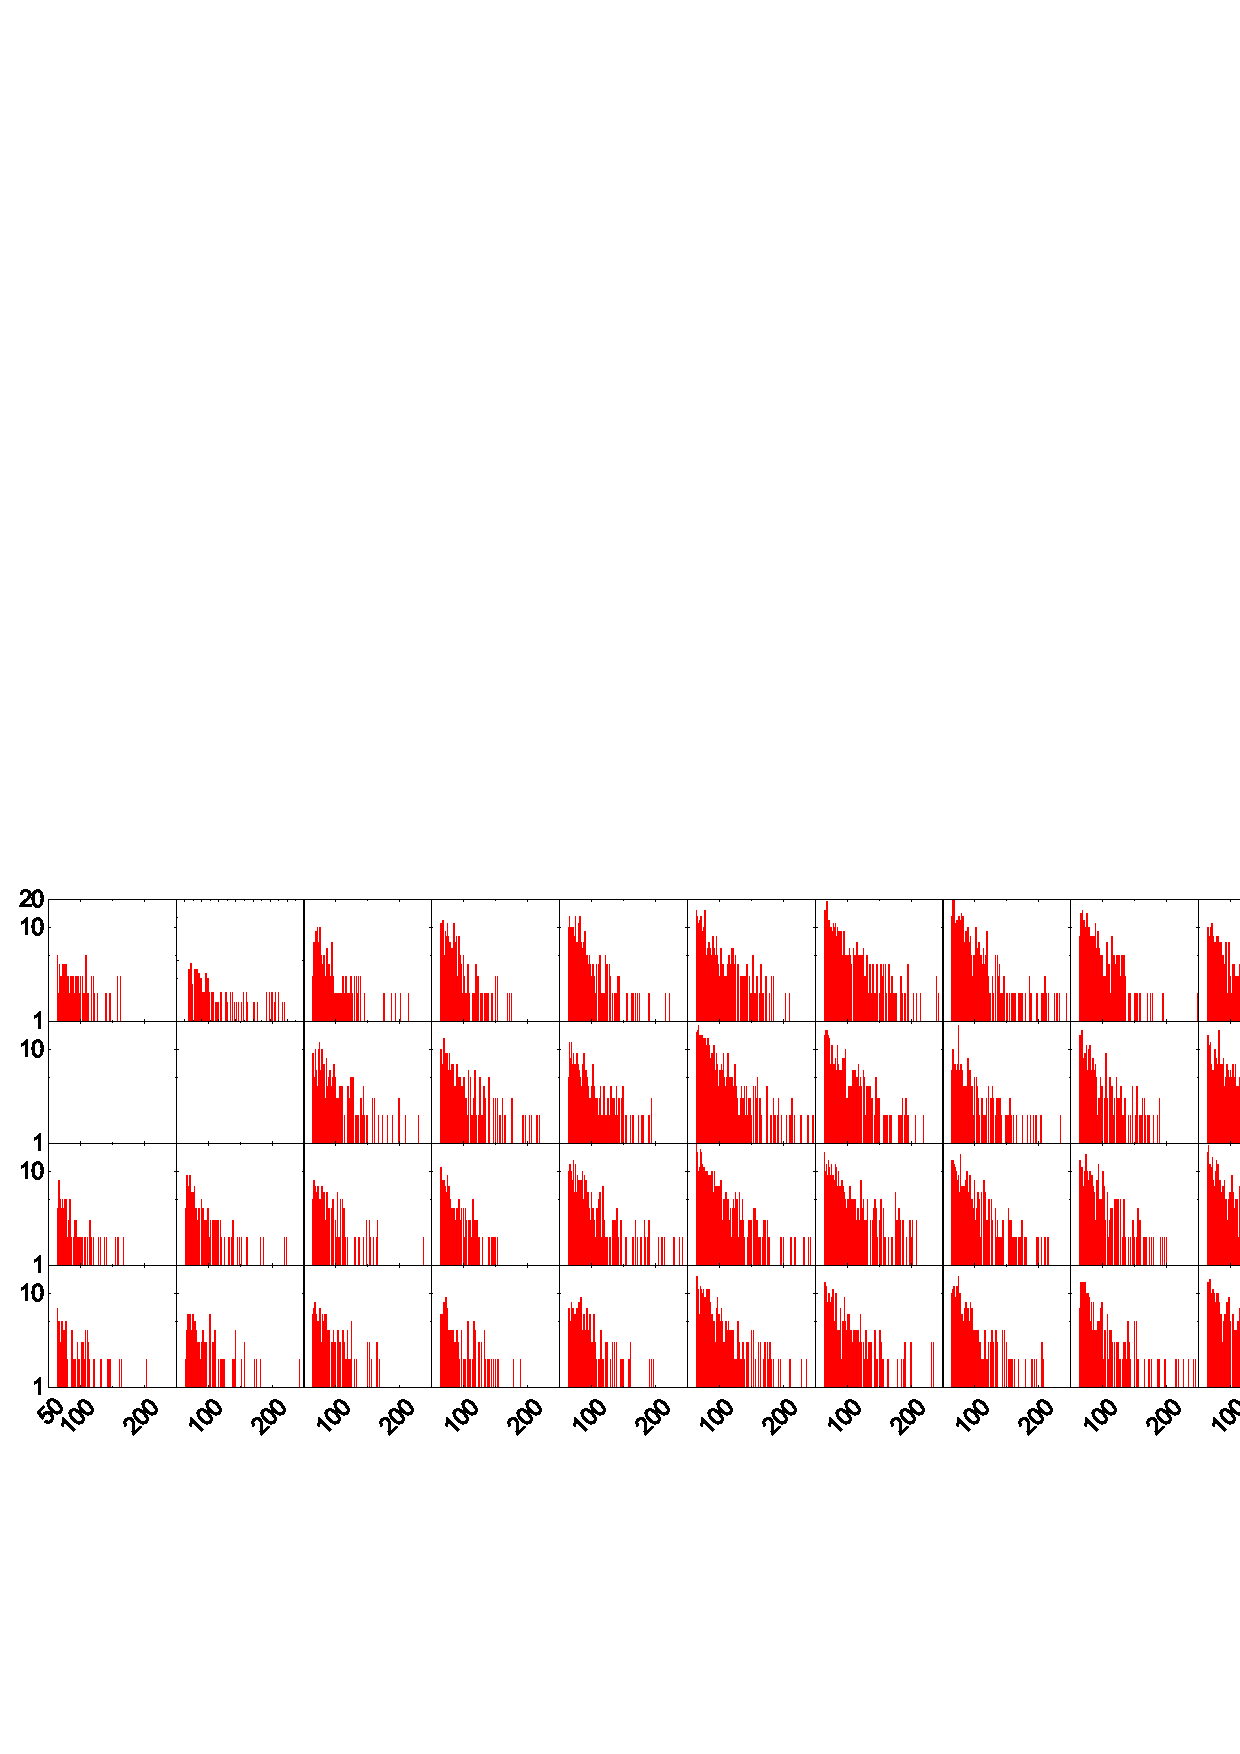
\includegraphics[width=\textwidth]{chapters/figures/flow_burst_size_48_spots.jpg}
\caption{\label{fig:flow_burst_size_48_spots}
Burst size histograms of all photons streams for each spot in the \ac{HT-smFRET} microfluidic experiment discussed in Section~\ref{sec:smFRET_microfluidics}. 
Analysis parameters: \ac{APBS}, $m = 10$, $r_m \geq 80~kHz$,
$\overline{F} \geq 64$. 
Spot 1 is at the top left, spot 12 at the top right. 
Spot 13 and 14 are missing from this series,
due to a malfunction of two SPADs in the donor SPAD array. 
The better illumination of the center spots translates into larger burst statistics.
Details of the analysis can be found in \texttt{ALiX Notebook, Flow, \ac{APBS}, m= 10, Rmin = 80 kHz, Smin = 64.rtf} and associated files in the Figshare repository~\cite{figshare_repo_2019}. 
Figure reprinted from Segal, \textit{et al.}~\cite{segal_methods_2019}.
}
\end{figure}

When the characteristics of different spots are comparable, it is reasonable to combine this data into a unified histogram. 
This approach is illustrated in Fig.~\ref{fig:pooled_burst_size_distributions}, facilitating comparisons between datasets acquired under identical conditions or to assess the impact of various burst search parameters on the burst size distribution.

\begin{figure}
\centering\includegraphics[width=0.7\textwidth]{chapters/figures/pooled_burst_size_distributions.jpg}
\caption{\label{fig:pooled_burst_size_distributions}
Pooled burst size histograms corresponding to the two datasets discussed in section \ref{sec:smFRET_microfluidics}. 
The diffusion only (no flow or \enquote{NF}) dataset, recorded with lower excitation powers (by a factor $\sim1.6$), was analyzed with a lower rate threshold ($r_m \geq 50~kHz$) for burst search and a lower burst size threshold ($\overline{F} \geq 40$, black)
for burst selection, than the dataset recorded with flow (F, red), for which $r_m \geq 80~kHz = 50 \times 1.6, \overline{F} \geq 64 = 40 \times 1.6$, in order to obtain comparable number of bursts for analysis.
For comparison, burst size distributions obtained when using the larger rate threshold for the no flow sample ($r_m \geq 80~kHz$,  NF, gray), or the lower burst size threshold for the sample with flow ($\overline{F} \geq 40$, F, orange) are represented as dashed curves. The red curve corresponds to the sum of all histograms in
Figure~\ref{fig:flow_burst_size_48_spots}.
The higher excitation powers used in the flow measurement more than compensate for the shorter transit time of molecules and more stringent burst search and selection criteria, as can be seen from the larger number and larger sizes of the collected bursts.
Details of the analysis can be found in the different notebooks: \texttt{ALiX Notebook, XX, \ac{APBS}, m = 10, Rmin = YY kHz, Smin = ZZ.rtf} where XX = Flow or No Flow, YY = 50 or 80, ZZ = 40 or 64, and associated files in the Figshare repository~\cite{figshare_repo_2019}. 
Figure reprinted from Segal, \textit{et al.}~\cite{segal_methods_2019}.
}
\end{figure}

\subsection{Burst Duration}
\label{sec:burst_duration_apdx}

Burst duration, as discussed earlier in the context of burst search, is a valuable parameter for a rapid assessment of potential differences in spot sizes or alignment. 
When observing the same sample across all spots, any expected scaling, assuming the spots are similar, should primarily manifest as differences in the number of bursts.
This could occur, for instance, if the excitation power is not uniform across the pattern. 
In such cases, the overall shape of the duration histograms should remain nearly identical, provided that an appropriate burst search using a constant threshold is performed~\cite{ingargiola_PLOS1_2016}. 
If the burst duration histograms exhibit dissimilarity, it is important to investigate potential sources of non-uniformities.

However, it is important to note that the burst duration distribution is a complex function for which no current analytical model exists. 
As discussed previously~\cite{ingargiola_PLOS1_2016}, a practical way to represent these intricate distributions is by using a modified semi-logarithmic histogram introduced by Sigworth and Sine~\cite{sigworth_BJ_1987}. 
This approach was originally developed to study sums of exponentials and offers the advantage of easily identifying the relevant time scale. 
In this \enquote{S\&S} representation, data is binned logarithmically without normalization to account for the variable widths of the bins, and the square root of each bin content is displayed. 
An example of burst duration histograms obtained in the microfluidic \ac{HT-smFRET} measurement discussed in Section~\ref{sec:smFRET_microfluidics} is presented in Fig.~\ref{fig:flow_burst_duration_48_spots}.

\begin{figure}
\centering
\includegraphics[width=\textwidth]{chapters/figures/flow_burst_duration_48_spots.jpg}
\caption{\label{fig:flow_burst_duration_48_spots}
Burst duration histograms in seconds for each spot in the \ac{smFRET} in flow experiment discussed
in Section~\ref{sec:smFRET_microfluidics}. 
Analysis parameters: \ac{APBS}, $m = 10$, $r_m \geq 80~kHz$, $\overline{F} \geq 64$. 
Spot 1 is at the top left, spot 12 at the top right. Spot 13 and 14 are missing from this series, due to a malfunction of two SPADs in the donor SPAD array. 
The better illumination of the center spots translates into larger burst statistics.
Details of the analysis can be found in the notebook \texttt{ALiX Notebook, Flow, \ac{APBS}, m = 10, Rmin = 80 kHz, Smin = 64.rtf}  and associated files in the Figshare repository \cite{figshare_repo_2019}.
Figure reprinted from Segal, \textit{et al.}~\cite{segal_methods_2019}
}
\end{figure}

Similarly to burst sizes, if the characteristics of the spots are similar, it is reasonable to combine this data into a single histogram. 
This approach, demonstrated in Fig.~\ref{fig:pooled_burst_duration}, allows for straightforward comparisons with data acquired under the same conditions.

\begin{figure}
\centering\includegraphics[width=0.7\textwidth]{chapters/figures/pooled_burst_duration.jpg}
\caption{\label{fig:pooled_burst_duration}
Pooled burst duration S \& S histograms corresponding to the two datasets discussed
in section \ref{sec:smFRET_microfluidics}. 
The diffusion only (no flow or NF) dataset, recorded with lower excitation powers (by a factor $\sim1.6$), was analyzed with a lower rate threshold ($r_m \geq 50~kHz$) for burst search and a lower burst size threshold ($\overline{F} \geq 40$, black) for burst selection, than the dataset recorded with flow (F, red), for which $r_m \geq 80~kHz = 50 \times 1.6, \overline{F} \geq 64 = 40 \times 1.6$, in order to obtain comparable number of bursts for analysis.
For comparison, burst durations obtained when using the larger rate threshold for the no flow sample  ($r_m \geq 80~kHz$, NF, gray), or the lower burst size threshold for the sample with flow ($\overline{F} \geq 40$, F, orange) are represented as well. 
The red curve corresponds to the sum of all histograms in Figure~\ref{fig:flow_burst_duration_48_spots}.
The different burst search and selection criteria for each experiment result in different burst duration distributions, illustrating the challenges associated with this type of analysis.
Details of the analysis can be found in the different notebooks: \texttt{ALiX Notebook, XX, \ac{APBS}, m = 10, Rmin = YY kHz, Smin = ZZ.rtf} where XX = Flow or No Flow, YY = 50 or 80, ZZ = 40 or 64, and associated files in the Figshare repository~\cite{figshare_repo_2019}).
Figure reprinted from Segal, \textit{et al.}~\cite{segal_methods_2019}
}
\end{figure}

\subsection{Peak Burst Count Rate}
\label{sec:peak_count_rate_apdx}

The characteristics of bursts, such as those discussed earlier, may be modeled by probability density distributions due to the diffusion of single molecules within the confocal excitation volume. 
In some cases, these distributions can be theoretically modeled, and under favorable conditions, they approach exponential behavior~\cite{gopich_JCP_2006}. 
However, the choice of burst search parameters, including the selection of the photon stream, the value of $m$, the use of fixed or adaptive thresholds, and the application of burst fusion, can impact the observed burst statistics. 
For instance, applying a higher threshold to a burst that starts and ends with low count rates will result in a smaller burst size with a shorter burst duration.

In contrast, the peak count rate within a burst, which represents the maximum photon detection rate using a specific number of photons, is typically determined within the burst itself and is not influenced by burst truncation at its edges.

Hence, while quantities like burst size are intricately linked to the precise trajectory of a molecule through the excitation \ac{PSF}, the peak count rate primarily reflects how closely the molecule's trajectory approached the excitation peak within the spot. 
Therefore, plotting this parameter with a histogram for all bursts provides more direct information about the peak excitation intensity in each spot, which is important for comparing different spots in a multispot setup.

The peak count rate, as defined in the Supporting Information of the FRETBursts publication~\cite{ingargiola_PLOS1_2016}, is:

\begin{equation}
\label{eqn:peak_count_rate}
r^{Y}_{X_{max}} = max(r_m(t_i))
\end{equation}

\noindent
where the $t_i$'s are timestamps within a burst and $r_m(t_i)$ 
is defined by Eqn.~\ref{eqn:local_rate}.

The definition provided in Eqn.~\ref{eqn:peak_count_rate} relies solely on the timestamps $t_i$ within a burst and the rate function $r_m(t_i)$ defined by Eqn.~\ref{eqn:local_rate}. 
However, it doesn't consider laser alternation or specify which excitation cycle a timestamp corresponds to. 
To include laser alternation, the peak count rate requires modification:

\begin{equation}
\label{eqn:peak_count_rate'}
r'^{Y}_{X_{max}} = max\left(\frac{m-2}{\Delta t^{(m)}_{j}} - (p -1)g\right)
\end{equation}

% \noindent
In this equation, $t_j$ and $t_{j+m-1}$ represent the timestamps marking the start and end of a burst, respectively. 
The parameter $g$ represents the minimum time between two donor excitation cycles, and $p$ signifies the number of alternation periods separating the burst.

As with other burst statistics, the outcome of the analysis of a multispot dataset includes a series of histograms for the burst peak count rate, as shown in Fig.~\ref{fig:flow_burst_peak_r_D_D_48_spots}.

\begin{figure}
\centering
\includegraphics[width=\textwidth]{chapters/figures/flow_burst_peak_r_D_D_48_spots.jpg}
\caption{\label{fig:flow_burst_peak_r_D_D_48_spots}
Burst peak count rate histograms during the D-excitation period and in the donor channel for each spot in the microfludic \ac{HT-smFRET} experiment discussed in Section~\ref{sec:smFRET_microfluidics}.
Analysis parameters: \ac{APBS}, $m = 10$, $r_m \geq 80~kHz$,
$\overline{F} \geq 64$. 
Spot 1 is at the top left, spot 12 at the top right. Spot 13 and 14 are missing from this series, due to a malfunction of two SPADs in the donor SPAD array. 
The better illumination of the center spots translates into larger number of bursts, but also larger peak burst rates.
Details of the analysis can be found in the notebook \texttt{ALiX Notebook, Flow, \ac{APBS}, m = 10, Rmin = 80 kHz, Smin = 64.rtf} and associated files in the Figshare repository \cite{figshare_repo_2019}.
Figure reprinted from Segal, \textit{et al.}~\cite{segal_methods_2019}.
}
\end{figure}

Pooling the burst peak count rates from all spots into a single histogram is useful for comparing different experiments, even if some border spots exhibit fewer and dimmer bursts, as can be seen from an examination of the spot intensity pattern shown in Fig.~\ref{fig:setup}. 
This pooled peak count rates are presented in Fig.~\ref{fig:pooled_burst_peak_r_D_D}.

\begin{figure}
\centering
\includegraphics[width=0.7\textwidth]{chapters/figures/pooled_burst_peak_r_D_D.jpg}
\caption{\label{fig:pooled_burst_peak_r_D_D}
Pooled burst peak count rate histograms during the D-excitation period and in the donor channel corresponding to the two datasets discussed in section \ref{sec:smFRET_microfluidics}.
The diffusion only (no flow or NF) dataset, recorded with lower excitation powers (by a factor $\sim1.6$), was analyzed with a lower rate threshold ($r_m \geq 50~kHz$) for burst search and a lower burst size threshold ($\overline{F} \geq 40$, black) for burst selection, than the dataset recorded with flow (F, red), for which $r_m \geq 80~kHz = 50 \times 1.6, \overline{F} \geq 64 = 40 \times 1.6$, in order to obtain comparable number of bursts for analysis.
For comparison, burst size distributions obtained when using the larger rate threshold for the no flow sample  ($r_m \geq 80~kHz$, NF, gray), or the lower burst size threshold for the sample with flow ($\overline{F} \geq 40$, F, orange) are represented as dashed curves. 
The red curve corresponds to the sum of all histograms in
Figure \ref{fig:flow_burst_peak_r_D_D_48_spots}.
As argued in the text, the asymptotic part of the burst peak count rate distribution is insensitive to the exact burst search and selection parameters used in the analysis, as is clear from the overlap of the exponential tails of the two no flow (NF, black and gray) and the two flow (F, red and orange) curves.
The ratio of the two exponential coefficients (F: 216 kHz and NF: 116 kHz, $F/NF = 1.9$) is approximately equal to the ratio of the donor laser  excitation powers used in the two measurements ($500/300 = 1.7$), as expected.
Details of the analysis can be found in the different notebooks:
\texttt{ALiX Notebook, XX, \ac{APBS}, m = 10, Rmin = YY kHz, Smin = ZZ.rtf} where XX = Flow or No Flow, YY = 50 or 80, ZZ = 40 or 64, and associated files in the Figshare repository~\cite{figshare_repo_2019}.
Figure reprinted from Segal, \textit{et al.}~\cite{segal_methods_2019}.
}
\end{figure}

\section{Fluorescence Correlation Analysis}
\label{sec:fcs_analysis_apdx}

\ac{FCS} can be performed on single or multispot setups to characterize the excitation-detection volumes sampled by the donor and acceptor, determine diffusion coefficients, brightness, and, when sufficient statistics are available, it can be utilized to study short time-scale dynamics~\cite{krichevsky_RPP_2002}. 
In the case of multispot experiments, \ac{FCS} analysis is particularly helpful in detecting otherwise challenging-to-quantify differences in spot characteristics. 
One of the simplest pieces of information that can be readily extracted from this analysis is the diffusion time through the excitation-detection volume, $\tau_D$, which is a useful indication of variations between spots.

In previous studies, we have conducted comparisons of single and multispot setups using FCS analysis~\cite{colyer_BOE_2010,ingargiola_PLOS1_2016, ingargiola_JCP_2018}. 
This analysis can be performed on the same dye, resulting in the \ac{ACF}, or on two different dyes, leading to the \ac{CCF}.
\ac{CCF} analysis can also be performed using a single dye, as in the case of \ac{ACF}, however, these measurements require a optical beamsplitter for detection in two separate channels.
\ac{FCS} analysis is complementary to burst duration and brightness analysis, as it can be used to reveal subtle differences in effective excitation-detection volumes or peak excitation intensities~\cite{ingargiola_PLOS1_2016}.

Quantitative \ac{FCS} analysis can be affected by various experimental artifacts and may require simplifying assumptions that are not always met~\cite{hess_BJ_2002, enderlein_CPB_2004}. 
One significant challenge is that current \ac{SPAD} arrays can exhibit afterpulsing and other effects at short time scales ($< 1 \mu$s), which complicates the routine use of the \ac{ACF} as a tool for analysis using \ac{SPAD} detectors.

\ac{CCF} analysis, in contrast, can alleviate many of these issues. 
In \ac{smFRET} experiments with two detection channels, it is primarily limited to correlating donor and acceptor signals within a spot. 
However, when examining separate spots, there are no such limitations. 
In diffusion experiments, cross-correlating signals from different spots might not provide information on a sample, as the distance between spots is typically on the order of $5~\mu$m, which is too large to extract meaningful diffusion coefficient information. 
If analyzing the capabilities of a \ac{SPAD} array, \ac{CCF} analysis can be used to measure optical crosstalk between pixels within a single detection channel~\cite{ingargiola_PLOS1_2016, ingargiola_NIMA_2018}.

However, as demonstrated in Section~\ref{sec:microfluidics_CCF}, \ac{CCF} analysis between \ac{SPAD}s within a single detection channel can be effectively employed to extract flow velocity as well as the direction of flow~\cite{brinkmeier_AC_1999}. 
Additionally, by analyzing the average \ac{CCF} of all spots, enhanced statistical accuracy can be achieved, as illustrated in Fig.~\ref{fig:flow_analysis}. 

Future iterations of a multispot setup might incorporate two \ac{SPAD} arrays per channel, enabling \ac{CCF} analysis within single spots and channels. 
This advancement would provide access to short timescale dynamics. By appropriately accounting for spot-specific differences and averaging \ac{CCF} curves from multiple spots, the time required to accumulate sufficient statistics for studying short timescale dynamics could be significantly reduced~\cite{felekyan_RSI_2005}.


% citations in ACS style using achemso package
%\bibliographystyle{plain}

% Give this command the relative path to the .bib file.
\bibliography{bib.bib}

\end{document}
